%%%%%%%%%%%%%%%%%%%%%%%%%%%%%%%%%%%%%%%%%%%%%%%%%%%%%%%%%%%%%%%%%%%%%%
% DSSMV 2026: Technical Report
% CineTrack: Mobile Movie Catalog and Geospatial Cinema Mapping
% Authors: André Silva (1240567), Afonso Ferreira (1241013)
%%%%%%%%%%%%%%%%%%%%%%%%%%%%%%%%%%%%%%%%%%%%%%%%%%%%%%%%%%%%%%%%%%%%%%
\documentclass[runningheads,a4paper]{llncs}

\usepackage[utf8]{inputenc}
\usepackage[T1]{fontenc}
\usepackage{amssymb}
\setcounter{tocdepth}{3}
\usepackage{graphicx}
\usepackage{caption}
\usepackage{url}
\usepackage{array}
\usepackage{float}
\usepackage{enumitem}
\usepackage{listings}
\usepackage{xcolor}

\lstdefinestyle{javastyle}{
  language=Java,
  basicstyle=\ttfamily\scriptsize,
  keywordstyle=\bfseries\color{blue!70!black},
  commentstyle=\itshape\color{green!50!black},
  stringstyle=\color{red!60!black},
  numbers=left,
  numberstyle=\tiny,
  stepnumber=1,
  numbersep=6pt,
  breaklines=true,
  frame=single,
  tabsize=2,
  showstringspaces=false
}

\newcommand{\keywords}[1]{\par\addvspace\baselineskip
\noindent\keywordname\enspace\ignorespaces#1}

\begin{document}
\raggedbottom
\mainmatter

% ====================================================================
% TÍTULO E CABEÇALHOS
% ====================================================================
\title{CineTrack: Mobile Movie Catalog and Geospatial Cinema Mapping\\Technical Report}

\titlerunning{CineTrack: Technical Report}

% ====================================================================
% AUTORES
% ====================================================================
\author{
  Andr\'e Silva (1240567) \and
  Afonso Ferreira (1241013)
}

\authorrunning{A. Silva and A. Ferreira}

% ====================================================================
% AFILIAÇÃO
% ====================================================================
\institute{
  ISEP, Instituto Superior de Engenharia do Porto,\\
  Rua do Dr~Ant\'onio Bernardino de Almeida 431, 4249-015 Porto, Portugal\\
  \email{\{1240567,1241013\}@isep.ipp.pt}\\
  \url{https://www.isep.ipp.pt}
}

\toctitle{CineTrack: Technical Report}
\tocauthor{A. Silva and A. Ferreira}
\maketitle

% ====================================================================
% ABSTRACT
% ====================================================================
\begin{abstract}
This technical report documents the design, architecture, and implementation of \textbf{CineTrack} (\textit{ProjectDroid}), a native Android mobile application developed for the Software Development and Mobile Systems (\textit{DSSMV}) course unit within the Informatics and Telecommunications Engineering degree at ISEP. CineTrack unifies movie catalog discovery, personal collection management, and location-based cinema mapping into a responsive mobile experience. The report details the system's pure Java~21 domain model, technical glossary, class diagram, UI navigation flow, use case specifications, and design sequence diagrams. Furthermore, it describes the implementation of critical mobile engineering concerns: non-blocking asynchronous REST communication with The Movie Database (TMDB) and Foursquare Places APIs via Retrofit~2, realtime Cloud Firestore synchronization, hardware sensor integration (accelerometer-based \textit{Shake to Suggest} and native GPS positioning), OpenStreetMap (OSMDroid) interactive mapping with search radius overlays, and background battery preservation. Finally, automated JUnit~5 test suites and verification results on physical hardware are presented, demonstrating compliance with mobile engineering best practices and architectural standards.

\keywords{Android, Java 21, MVC Architecture, Cloud Firestore, Retrofit, Foursquare Places API, OSMDroid, Accelerometer Sensor, TMDB, DSSMV.}
\end{abstract}

\newpage

% ====================================================================
\section{Introduction}
% ====================================================================
The proliferation of digital streaming platforms has created an increasingly fragmented landscape for cinema enthusiasts seeking where specific titles are available for viewing or looking for physical screening rooms nearby. The \textbf{CineTrack} mobile application addresses this challenge by providing an integrated, responsive solution that merges remote cinematic catalogs, cloud-synced personal lists, hardware sensors, and geospatial mapping.

From an engineering perspective, developing robust software for mobile devices imposes strict architectural constraints due to limited physical resources, variable network connectivity, and the imperative requirement of maintaining graphical interface (\textit{UI Thread}) responsiveness. To prevent \textit{Application Not Responding} (ANR) dialogs and excessive battery depletion, CineTrack strictly follows four foundational mobile principles:
\begin{enumerate}[label=\textbf{\arabic*.}]
    \item \textbf{Model-View-Controller (MVC) Separation:} Pure Java~21 domain entities isolated from the Android SDK, enabling fast, isolated unit testing.
    \item \textbf{Non-Blocking I/O:} All network requests (Retrofit~2) and persistence updates are executed asynchronously off the main thread.
    \item \textbf{Sensor Lifecycle Discipline:} Hardware listeners for the accelerometer and GPS are registered exclusively in \texttt{onResume()} and immediately detached in \texttt{onPause()}.
    \item \textbf{Density-Independent UI Design:} Interface layouts in XML rely strictly on density-independent pixels (\texttt{dp}) and scale-independent pixels (\texttt{sp}).
\end{enumerate}

% ====================================================================
\section{Project Status}
% ====================================================================
The CineTrack project was developed collaboratively using a structured Git feature branch workflow, segregating tasks into two parallel development branches (\texttt{andre-1240567} and \texttt{afonso-1241013}) before integration into the \texttt{main} branch via peer-reviewed Pull Requests. Table \ref{tab:project-status} summarizes the implementation status and automated test coverage across all 11 User Stories.

\begin{table}[H]
\caption{CineTrack Implementation and Testing Status}
\label{tab:project-status}
\centering\small
\begin{tabular}{@{}>{\raggedright\arraybackslash}p{1.2cm}
                    >{\raggedright\arraybackslash}p{4.8cm}
                    >{\centering\arraybackslash}p{2.2cm}
                    >{\centering\arraybackslash}p{2.0cm}
                    >{\raggedright\arraybackslash}p{1.6cm}@{}}
\hline
\textbf{ID} & \textbf{User Story Description} & \textbf{Author} & \textbf{Status} & \textbf{Tests} \\
\hline
US1  & [Auth] User Registration and Sign-In       & André (1240567)  & 100\% Complete & Manual / Live \\
US2  & [CRUD] Create and Manage Movie Lists       & André (1240567)  & 100\% Complete & Unit / Mock \\
US3  & [CRUD] Add Movies and Submit Ratings       & André (1240567)  & 100\% Complete & 8 Unit Tests \\
US4  & [API] TMDB Search and Streaming Providers  & Afonso (1241013) & 100\% Complete & 6 Unit Tests \\
US5  & [Map] Nearby Cinemas (GPS + OSMDroid)      & Afonso (1241013) & 100\% Complete & 7 Unit Tests \\
US6  & [Sensor] Shake to Suggest (Accelerometer)  & Afonso (1241013) & 100\% Complete & 4 Unit Tests \\
US7  & [Auth] Profile Management and Sign-Out     & André (1240567)  & 100\% Complete & Manual / Live \\
US8  & [Persistence] Local Preferences (apply)   & Afonso (1241013) & 100\% Complete & 7 Unit Tests \\
US9  & [CRUD] Local Collection Filter and Sort    & André (1240567)  & 100\% Complete & 12 Unit Tests \\
US10 & [API] Official YouTube Video Trailers      & Afonso (1241013) & 100\% Complete & 4 Unit Tests \\
US11 & [Social] External Movie Card Sharing       & André (1240567)  & 100\% Complete & Manual / Live \\
\hline
\textbf{Total} & \multicolumn{3}{l}{\textbf{All 11 User Stories Fully Implemented and Merged}} & \textbf{53 Passing} \\
\hline
\end{tabular}
\end{table}

\newpage

% ====================================================================
\section{Domain Model}
% ====================================================================
The conceptual Domain Model defines the business entities and structural relationships of CineTrack independent of technological frameworks. As illustrated in Figure \ref{fig:dm}, the domain revolves around the central concepts of authenticated users, personal movie lists, saved movies, watch states, ratings, and physical cinema points of interest.

\begin{figure}[H]
    \centering
    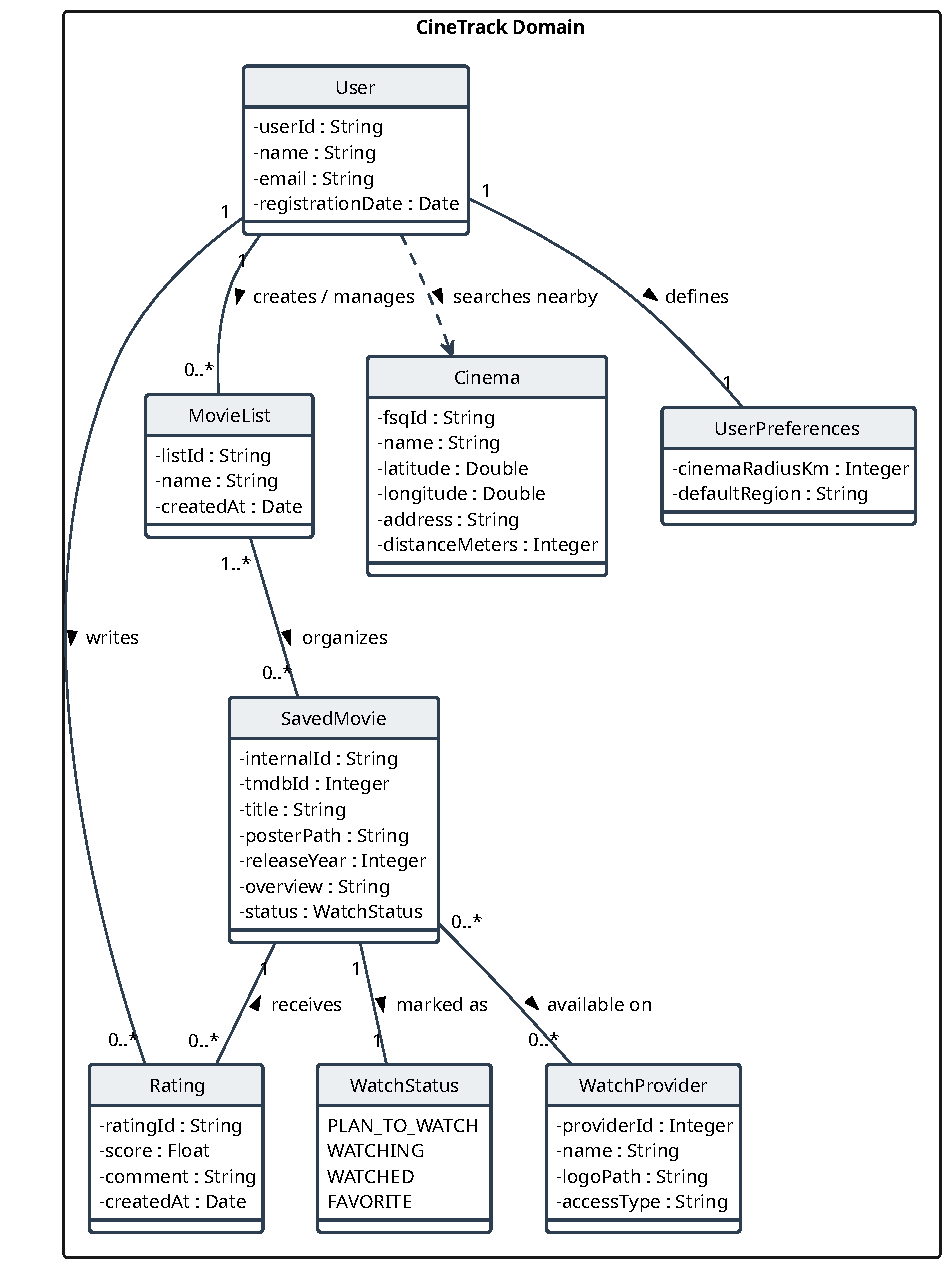
\includegraphics[width=0.95\textwidth]{figures/global-artifacts/DM.pdf}
    \caption{CineTrack Conceptual Domain Model}
    \label{fig:dm}
\end{figure}

The domain model enforces several essential business invariants:
\begin{itemize}
    \item \textbf{User and MovieList Ownership:} A \texttt{User} uniquely owns zero or more \texttt{MovieList} entities. Each list contains an arbitrary number of \texttt{SavedMovie} instances.
    \item \textbf{WatchStatus Progression:} Every saved movie is categorized under a strict enumeration: \texttt{PLAN\_TO\_WATCH}, \texttt{WATCHING}, \texttt{WATCHED}, or \texttt{FAVORITE}.
    \item \textbf{Rating Interval:} A \texttt{Rating} score must strictly satisfy $1.0 \le \text{score} \le 5.0$. Values outside this range throw checked \texttt{InvalidRatingException} instances.
    \item \textbf{Geospatial Radius Bounds:} The user's search radius for cinemas must lie within $1 \le \text{radius} \le 100$ kilometers.
\end{itemize}

\newpage

% ====================================================================
\section{Glossary}
% ====================================================================
Table \ref{tab:glossary} establishes the standard technical and domain terminology used throughout the CineTrack documentation and implementation.

\begin{table}[H]
\caption{CineTrack Technical and Domain Glossary}
\label{tab:glossary}
\centering\scriptsize
\begin{tabular}{@{}>{\raggedright\arraybackslash}p{2.8cm}
                    >{\raggedright\arraybackslash}p{2.8cm}
                    >{\raggedright\arraybackslash}p{6.2cm}@{}}
\hline
\textbf{Term/Expression (EN)} & \textbf{Termo (PT)} & \textbf{Definition/Description} \\
\hline
ANR & Falha por Inatividade & Application Not Responding dialog triggered by Android when the UI Thread remains blocked for more than 5 seconds. \\[3pt]
Cinema & Sala de Cinema & Physical point of interest possessing latitude, longitude, formatted address, and distance, queried from Foursquare Places API. \\[3pt]
Explicit Intent & Intent Explícito & Navigation message explicitly designating an internal Activity class within the application package. \\[3pt]
Foursquare Places API & API Foursquare & REST service providing geospatial POI search by geographic coordinates and category (Cinema category \texttt{10024}). \\[3pt]
Implicit Intent & Intent Implícito & Abstract action delegated to the Android operating system to resolve via external installed applications (e.g., Google Maps, YouTube). \\[3pt]
MovieList & Lista de Filmes & Personalized user collection stored in Cloud Firestore (e.g., "Favorites", "Watchlist"). \\[3pt]
MVC & Padrão MVC & Architectural pattern separating pure Java Model entities, declarative XML Views, and Activity Controllers. \\[3pt]
OSMDroid & OpenStreetMap SDK & Open-source Android library for rendering map tiles, circle overlays, and clickable marker pins without paid API keys. \\[3pt]
Rating & Avaliação & Quantitative score in the interval $[1.0, 5.0]$ and optional qualitative review text. \\[3pt]
Retrofit 2 & Cliente Retrofit & Type-safe HTTP client abstracting asynchronous REST API invocations via \texttt{.enqueue()} and Gson serialization. \\[3pt]
SavedMovie & Filme Guardado & Domain representation of a movie linked to a list, containing TMDB identifier, title, release year, poster URL, and watch status. \\[3pt]
ShakeDetector & Detetor de Agitação & Custom \texttt{SensorEventListener} detecting deliberate multi-peak accelerations ($>2.7g$) while ignoring incidental vibrations. \\[3pt]
SharedPreferences & Preferências Locais & Lightweight key-value persistence. Writing operations strictly use asynchronous \texttt{.apply()} to avoid UI Thread locking. \\[3pt]
TMDB & The Movie Database & External REST service supplying cinematic catalog discovery, streaming watch providers by country, and official trailers. \\[3pt]
UI Thread & Thread Principal & Android's main execution thread responsible for screen rendering and touch events; must never execute blocking I/O. \\[3pt]
WatchProvider & Fornecedor de Streaming & Licensed digital streaming service (e.g., Netflix, HBO Max, Disney+) available in the selected geographical region. \\
\hline
\end{tabular}
\end{table}

\newpage

% ====================================================================
\section{Design}
% ====================================================================

\subsection{Model - Class Diagram}
Figure \ref{fig:cd} depicts the core class diagram of the pure Java~21 domain layer located in \texttt{pt.isep.dssmv.projectdroid.model}. The domain layer maintains strict independence from all Android SDK packages.

\begin{figure}[H]
    \centering
    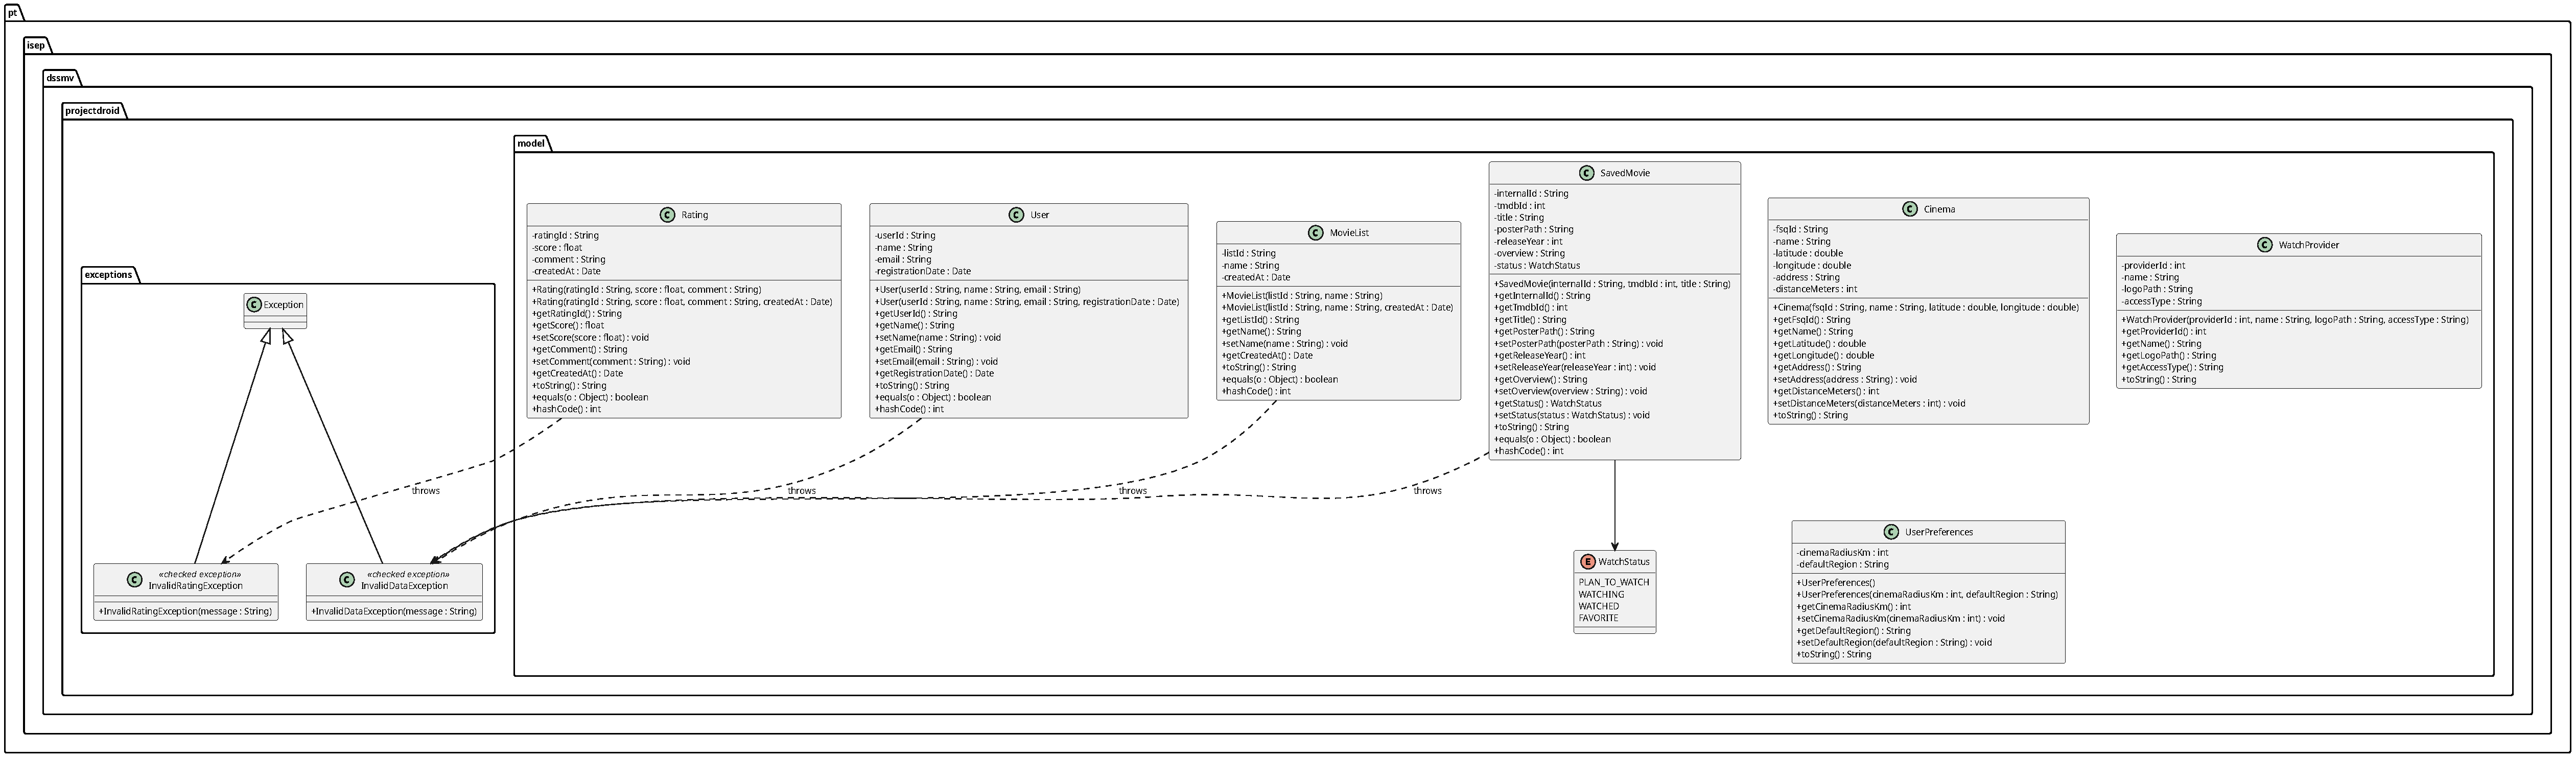
\includegraphics[width=0.95\textwidth]{figures/global-artifacts/CD.pdf}
    \caption{Implementation Class Diagram: Pure Java 21 Domain Model}
    \label{fig:cd}
\end{figure}

\subsection{User Interface Flow}
Figure \ref{fig:ui-flow} illustrates the screen transitions and navigation flow across all activities within the application.

\begin{figure}[H]
    \centering
    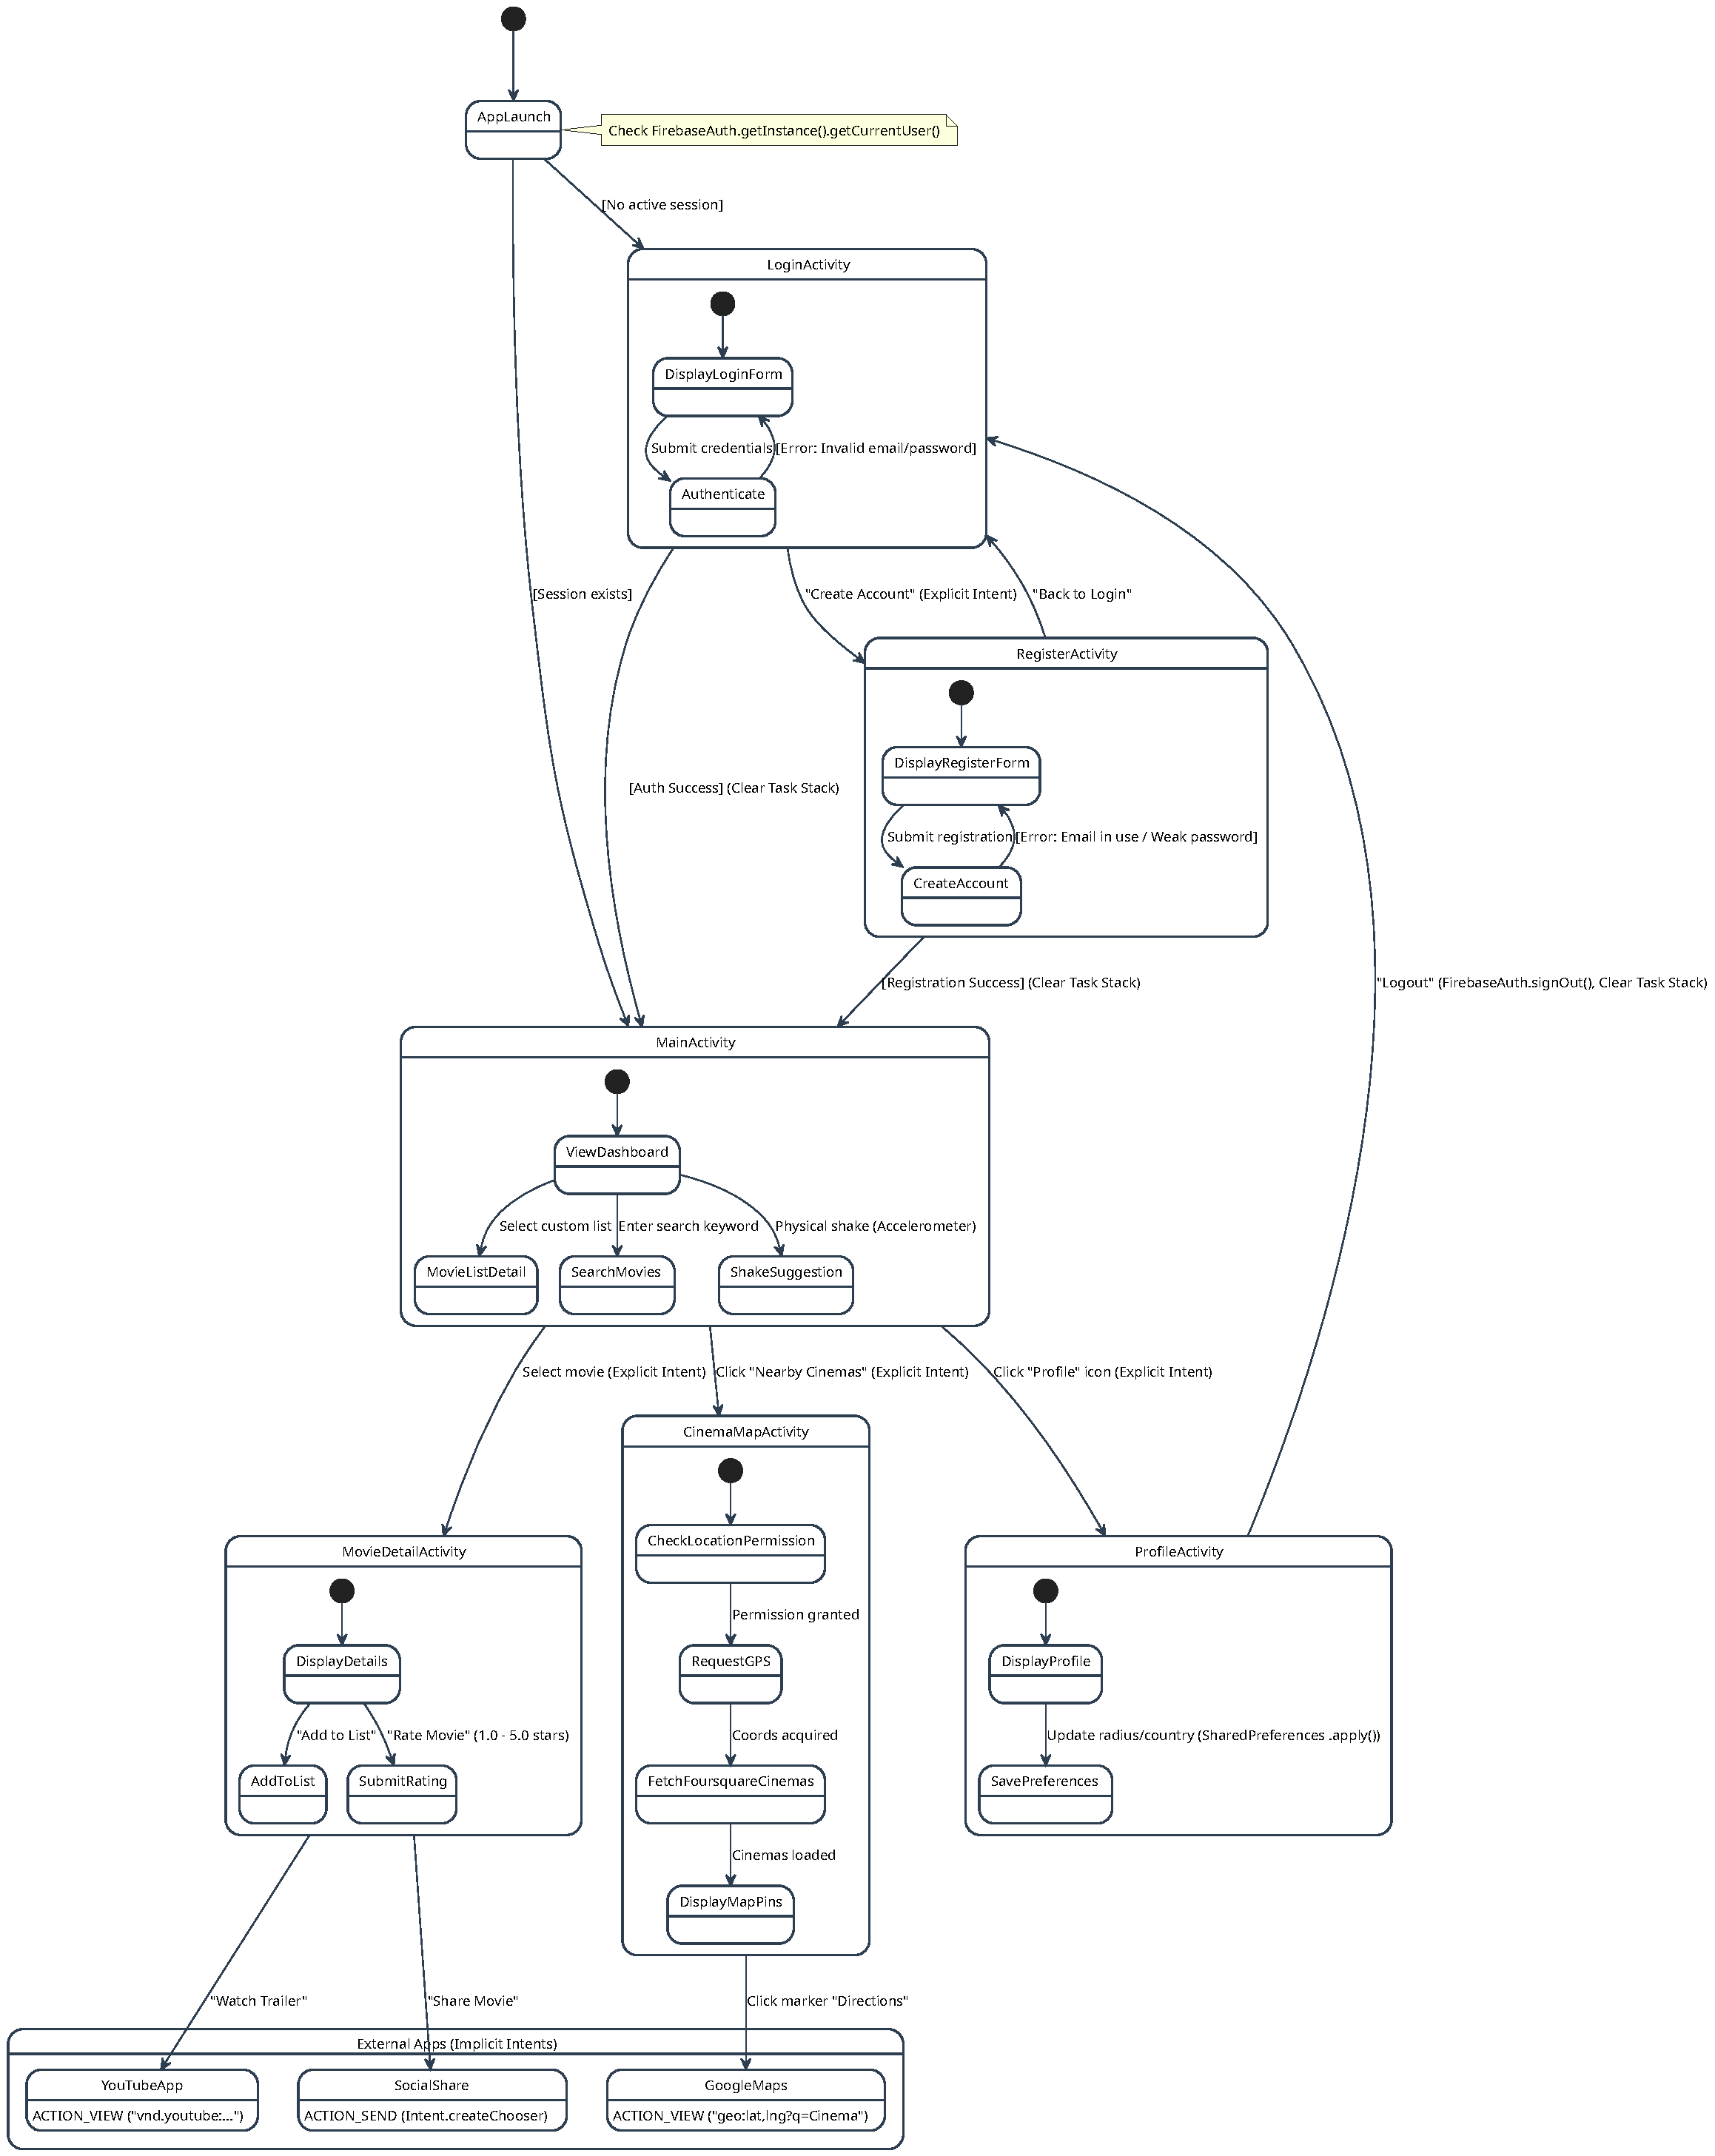
\includegraphics[width=0.90\textwidth]{figures/global-artifacts/UI_Flow.pdf}
    \caption{UI Navigation Flow and Activity Transitions}
    \label{fig:ui-flow}
\end{figure}

\newpage

\subsection{Use Case Diagrams}
Figure \ref{fig:ucd-global} provides the global Use Case Diagram, decomposing CineTrack into four functional subsystems and illustrating connections to supporting cloud services, hardware sensors, and external applications.

\begin{figure}[H]
    \centering
    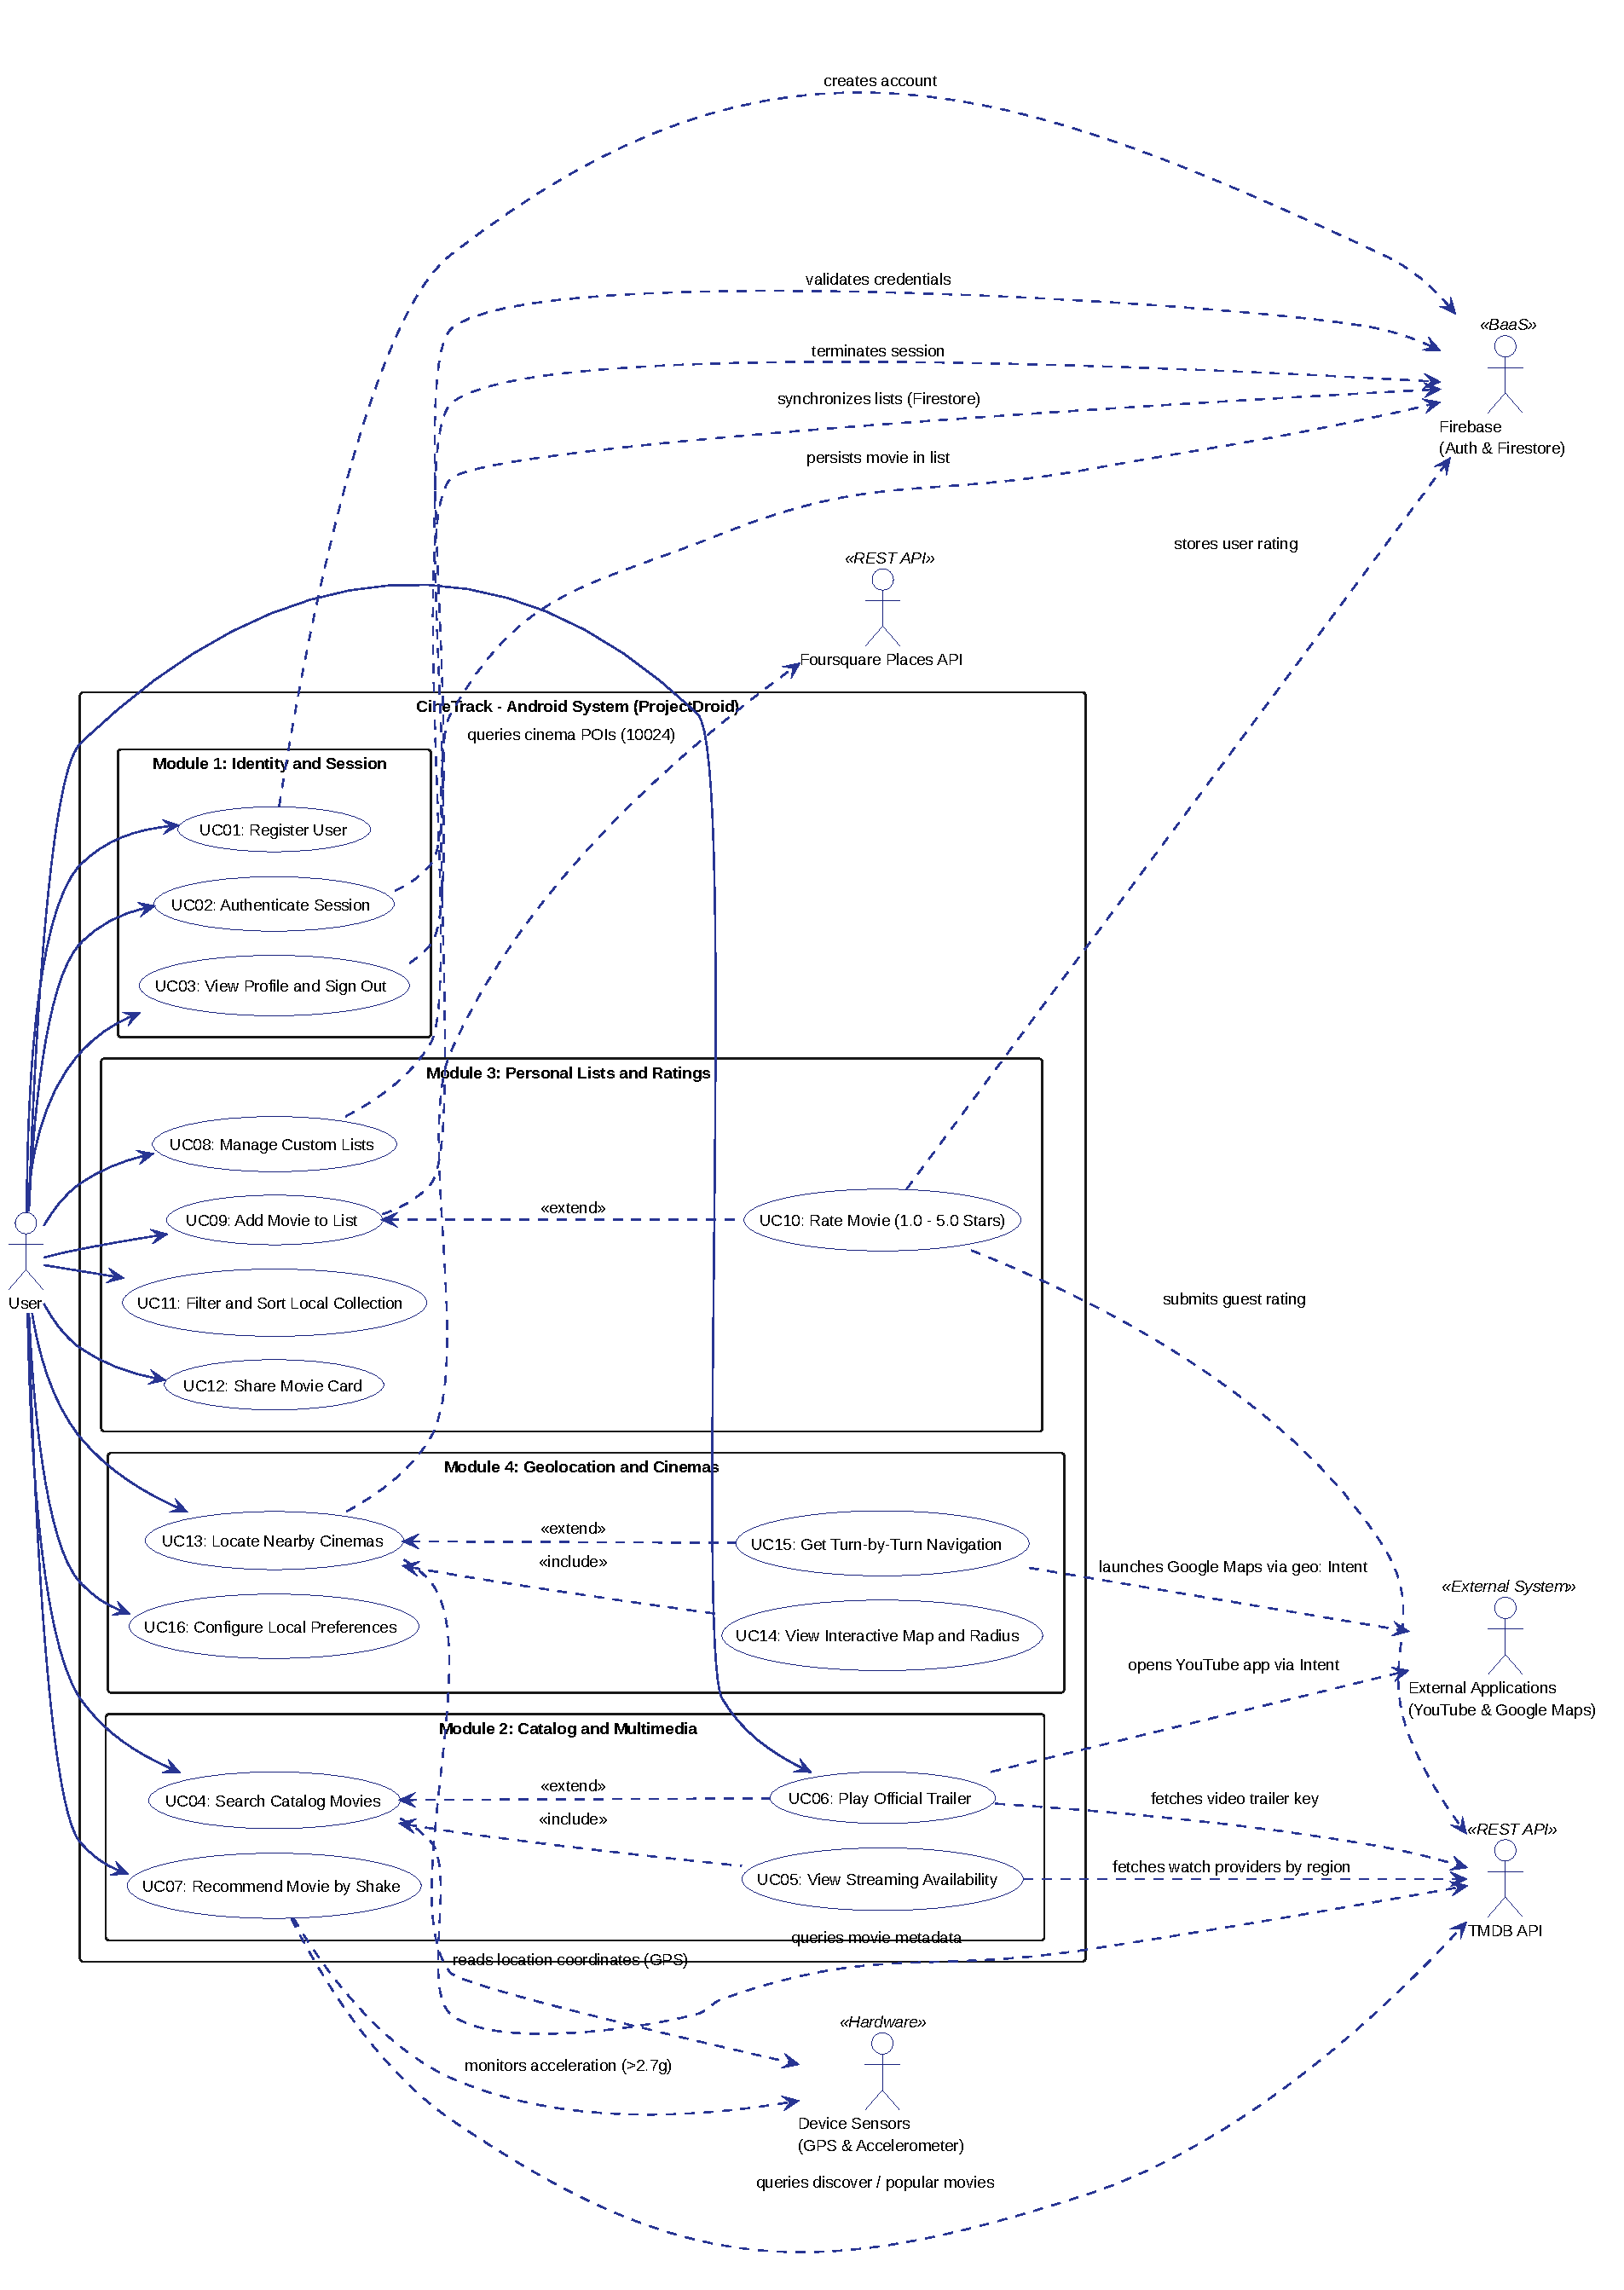
\includegraphics[width=0.85\textwidth]{figures/global-artifacts/UCD_Global.pdf}
    \caption{Global System Use Case Diagram}
    \label{fig:ucd-global}
\end{figure}

Figures \ref{fig:ucd-discovery}, \ref{fig:ucd-cinemas}, and \ref{fig:ucd-lists} detail the modular subsystems, highlighting internal \texttt{<<include>>} and \texttt{<<extend>>} relationships.

\begin{figure}[H]
    \centering
    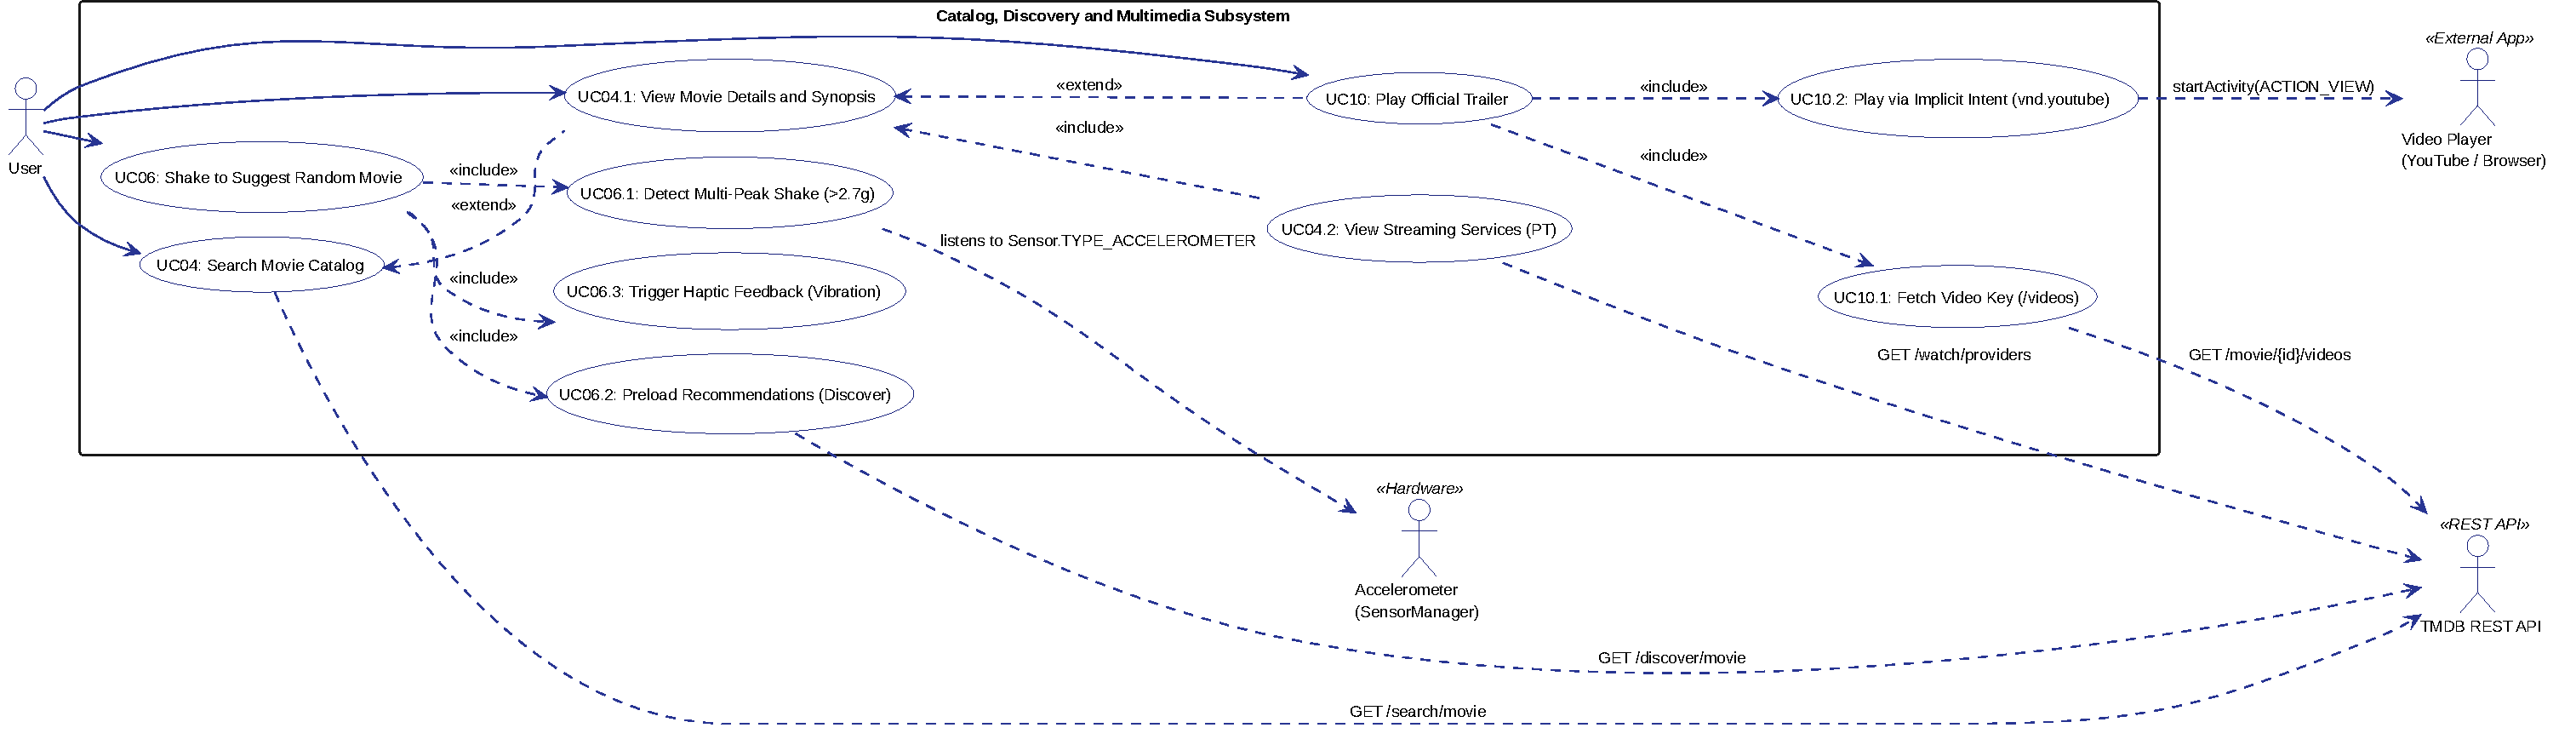
\includegraphics[width=0.75\textwidth]{figures/global-artifacts/UCD_Discovery.pdf}
    \caption{UCD: Catalog, Discovery and Multimedia Subsystem}
    \label{fig:ucd-discovery}
\end{figure}

\begin{figure}[H]
    \centering
    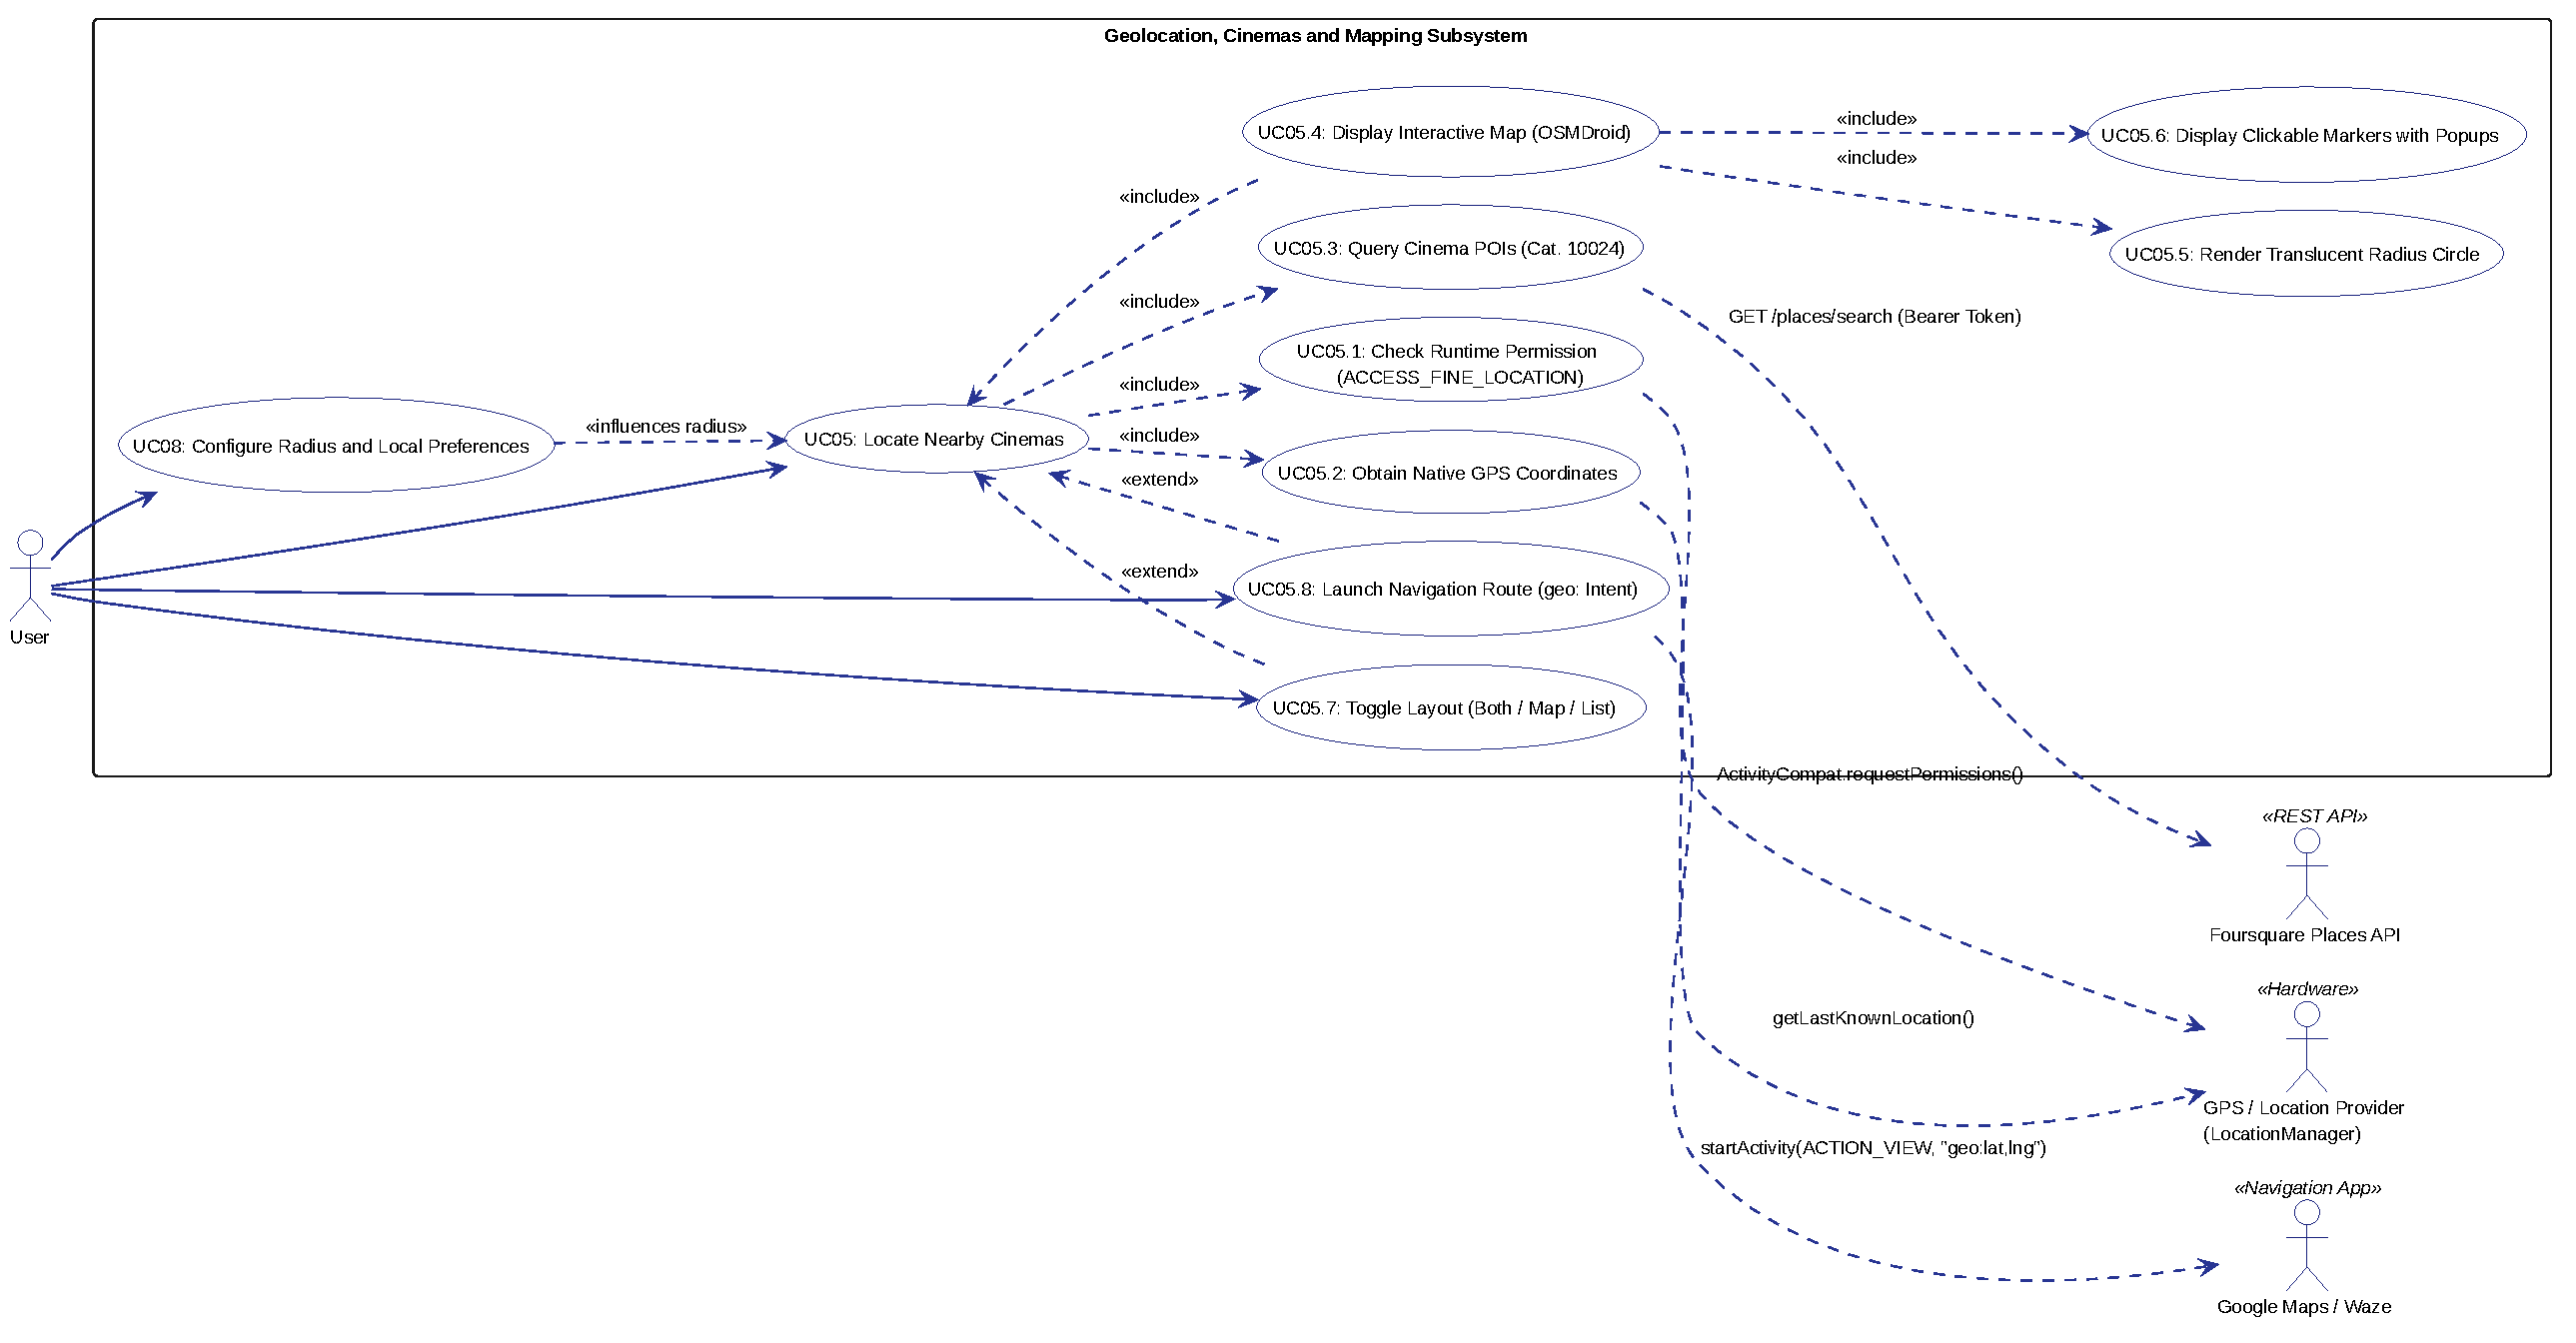
\includegraphics[width=0.75\textwidth]{figures/global-artifacts/UCD_Cinemas.pdf}
    \caption{UCD: Geospatial Mapping and Cinemas Subsystem}
    \label{fig:ucd-cinemas}
\end{figure}

\begin{figure}[H]
    \centering
    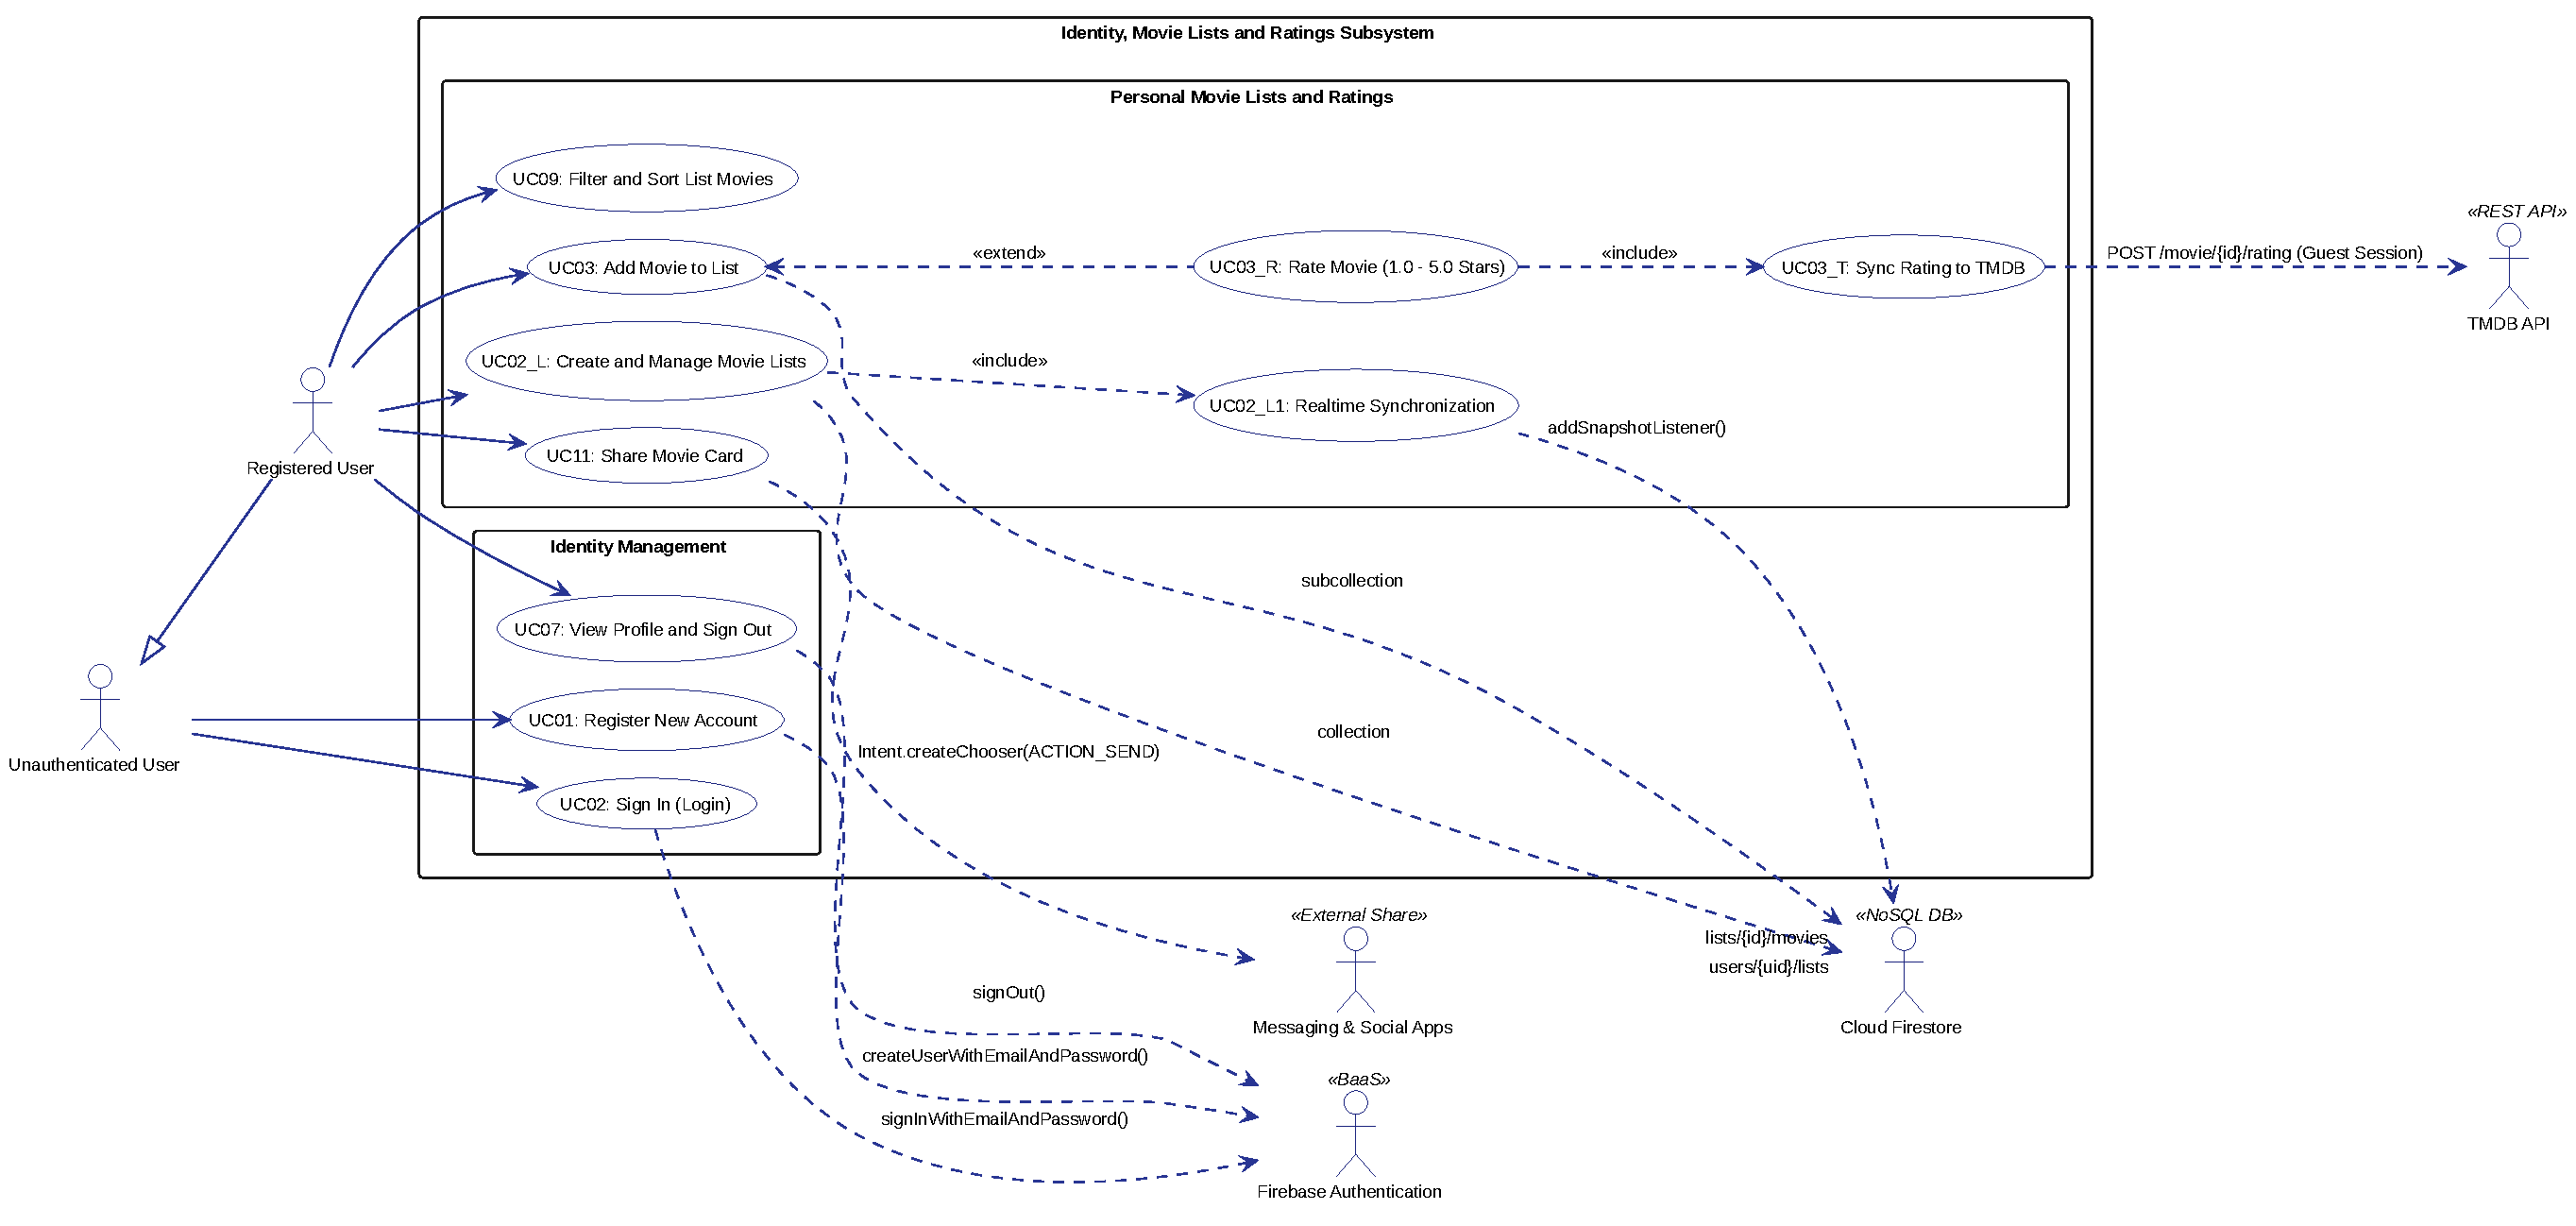
\includegraphics[width=0.75\textwidth]{figures/global-artifacts/UCD_Lists.pdf}
    \caption{UCD: Identity, Movie Lists and Ratings Subsystem}
    \label{fig:ucd-lists}
\end{figure}

\newpage

\subsection{Sequence Diagrams}

% --------------------------------------------------------------------
% UC1
% --------------------------------------------------------------------
\vspace{0.2cm}
\noindent{\Large \textbf{Use Case 1: User Registration and Authentication}}
\vspace{0.2cm}

The specification for UC1 is detailed in Table \ref{tab:uc1}, and its execution flow is represented in Figure \ref{fig:uc1-sd}.

\begin{center}
    \small
    \captionof{table}{Use Case 1: User Registration and Sign-In} \label{tab:uc1}
    \vspace{4pt}
    \begin{tabular}{@{}>{\raggedright\arraybackslash}p{2.8cm}
            >{\raggedright\arraybackslash}p{8.8cm}@{}}
        \hline
        \textbf{Actor}          & User (Unauthenticated / Registered) \\
        \hline
        \textbf{Use case name}  & User Registration and Sign-In \\
        \textbf{Description}    & Allows the user to register an account or sign into an existing account using email and password via Firebase Authentication. \\
        \textbf{Precondition}   & Network connectivity must be available; device is on the login/register screen. \\
        \textbf{Post-condition} & Active session token established; user navigated to MainActivity with clear-task flags. \\
        \textbf{Main flow}      & 
        1. User inputs email and password and triggers the login action. \newline
        2. System validates input formats locally. \newline
        3. System submits asynchronous sign-in request to Firebase Auth. \newline
        4. Firebase validates credentials and returns authenticated user token. \newline
        5. System clears login activity from backstack and launches MainActivity. \\
        \textbf{Alternative path} & 
        If credentials are invalid or network fails, Firebase returns an error task; system clears progress bar and presents an informative toast to the user. \\
        \hline
    \end{tabular}
\end{center}

\begin{figure}[H]
    \centering
    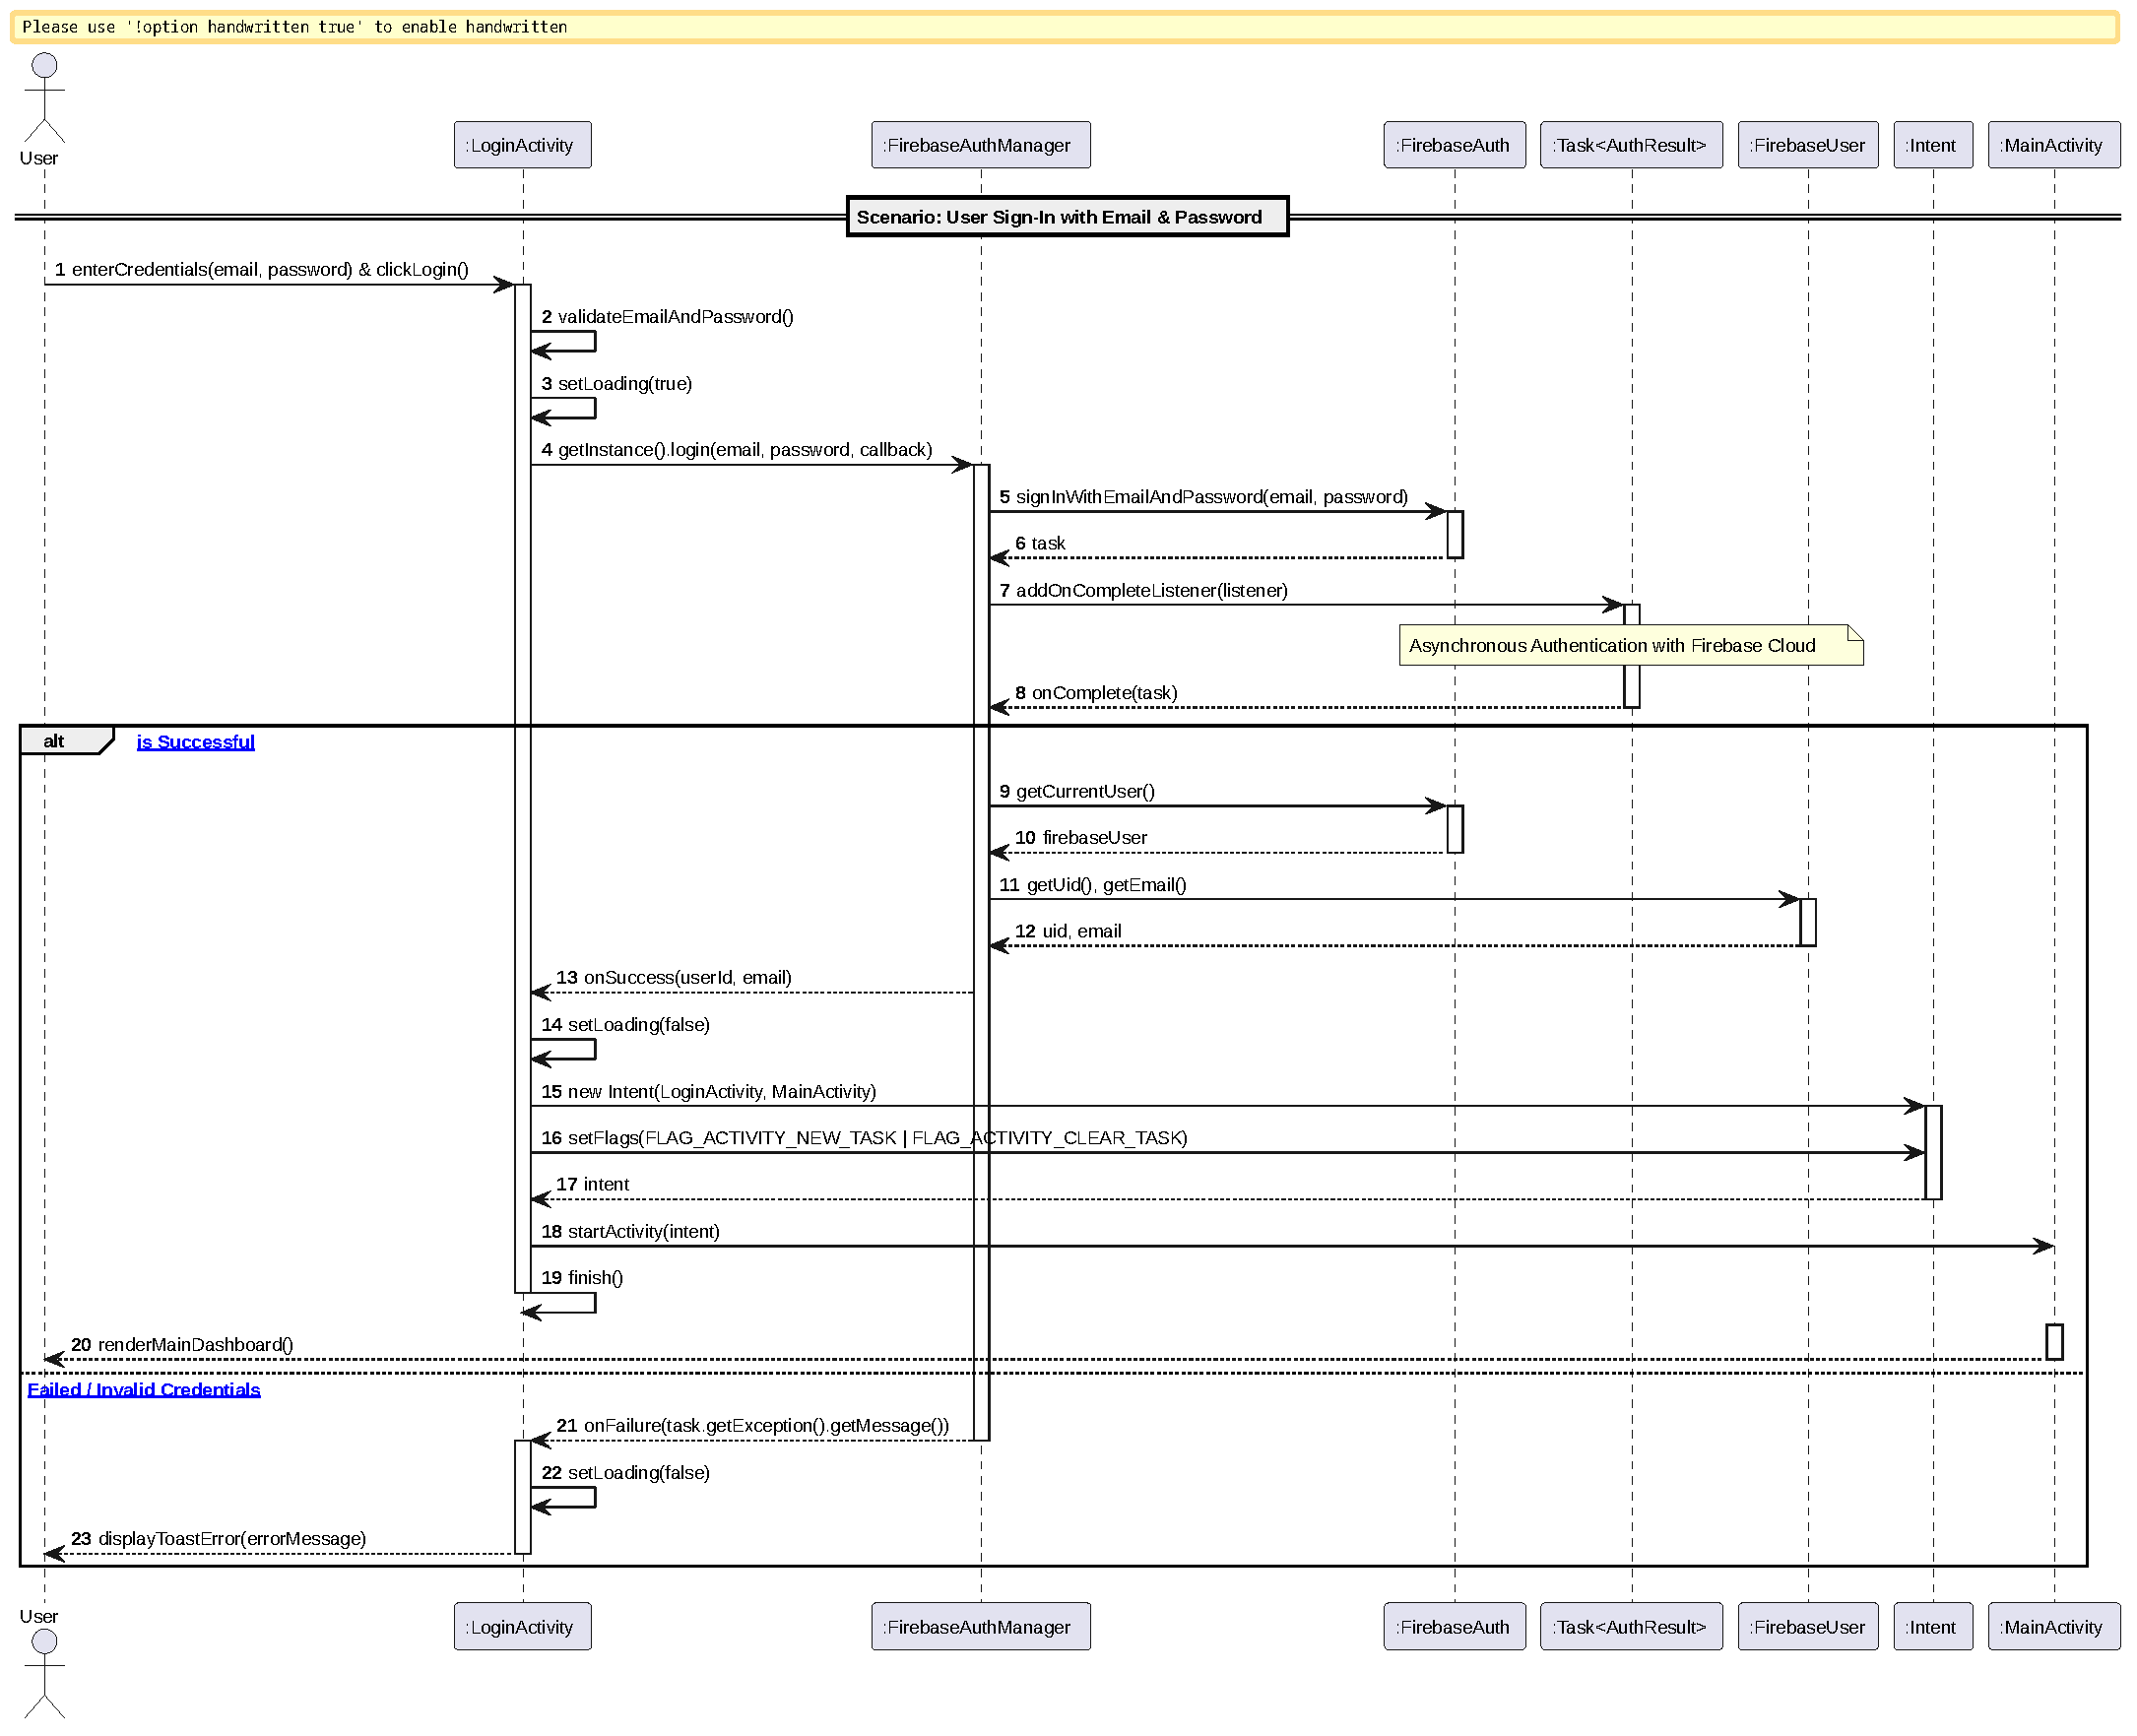
\includegraphics[width=0.85\textwidth]{figures/Use_Cases/UC1-SD.pdf}
    \caption{UC1: User Authentication Design Sequence Diagram}
    \label{fig:uc1-sd}
\end{figure}

\newpage

% --------------------------------------------------------------------
% UC2
% --------------------------------------------------------------------
\vspace{0.2cm}
\noindent{\Large \textbf{Use Case 2: Create and Manage Movie Lists}}
\vspace{0.2cm}

The specification for UC2 is detailed in Table \ref{tab:uc2}, and its execution flow is represented in Figure \ref{fig:uc2-sd}.

\begin{center}
    \small
    \captionof{table}{Use Case 2: Create and Manage Movie Lists} \label{tab:uc2}
    \vspace{4pt}
    \begin{tabular}{@{}>{\raggedright\arraybackslash}p{2.8cm}
            >{\raggedright\arraybackslash}p{8.8cm}@{}}
        \hline
        \textbf{Actor}          & Authenticated User \\
        \hline
        \textbf{Use case name}  & Create and Manage Movie Lists \\
        \textbf{Description}    & Allows an authenticated user to create personal movie lists and observe realtime synchronization across devices via Cloud Firestore. \\
        \textbf{Precondition}   & User must be signed into a valid account. \\
        \textbf{Post-condition} & A new list document is added to Firestore; realtime listener updates the RecyclerView. \\
        \textbf{Main flow}      & 
        1. User opens the "My Lists" tab and taps the add list button. \newline
        2. System displays dialog modal requesting the list name. \newline
        3. User enters the list name and confirms. \newline
        4. System instantiates a pure MovieList domain entity. \newline
        5. FirestoreManager writes the document to \texttt{users/\{uid\}/lists/\{id\}}. \newline
        6. Firestore realtime snapshot listener automatically detects the new record and updates UI. \\
        \textbf{Alternative path} & 
        If the list name is empty or Firestore write fails, system alerts the user and keeps the dialog open. \\
        \hline
    \end{tabular}
\end{center}

\begin{figure}[H]
    \centering
    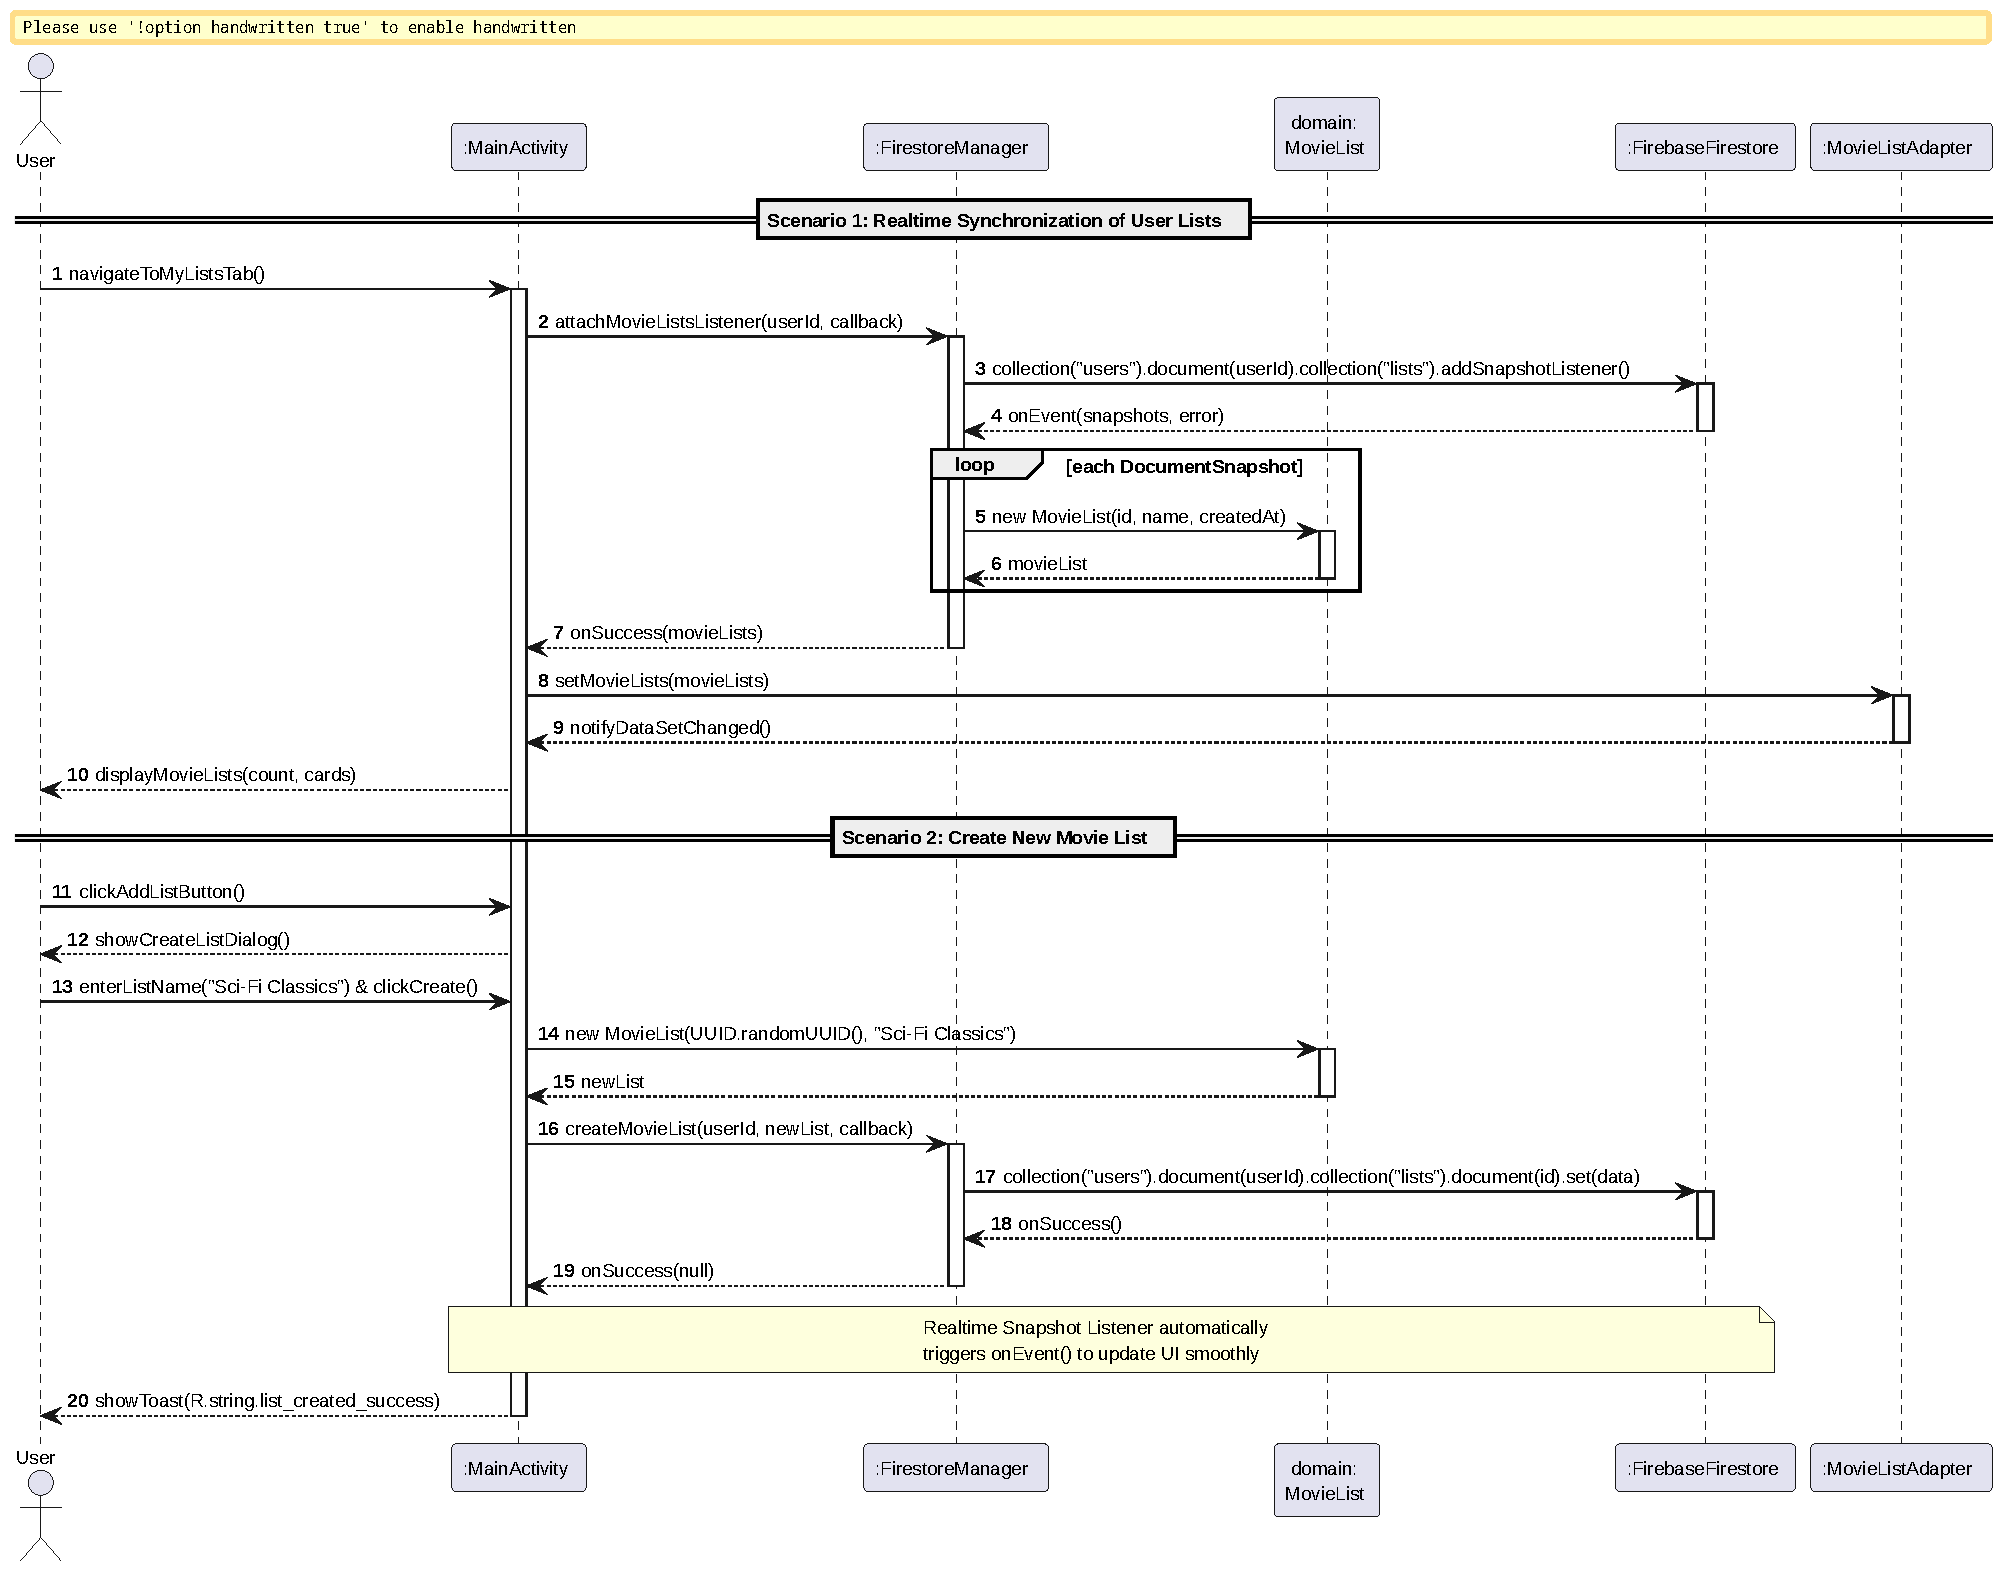
\includegraphics[width=0.85\textwidth]{figures/Use_Cases/UC2-SD.pdf}
    \caption{UC2: Manage Lists Design Sequence Diagram}
    \label{fig:uc2-sd}
\end{figure}

\newpage

% --------------------------------------------------------------------
% UC3
% --------------------------------------------------------------------
\vspace{0.2cm}
\noindent{\Large \textbf{Use Case 3: Add Movie to List and Submit Rating}}
\vspace{0.2cm}

The specification for UC3 is detailed in Table \ref{tab:uc3}, and its execution flow is represented in Figure \ref{fig:uc3-sd}.

\begin{center}
    \small
    \captionof{table}{Use Case 3: Add Movie and Rate} \label{tab:uc3}
    \vspace{4pt}
    \begin{tabular}{@{}>{\raggedright\arraybackslash}p{2.8cm}
            >{\raggedright\arraybackslash}p{8.8cm}@{}}
        \hline
        \textbf{Actor}          & Authenticated User \\
        \hline
        \textbf{Use case name}  & Add Movie to List and Submit Rating \\
        \textbf{Description}    & Allows the user to save a movie into a selected personal list, set its watch status, and submit a rating (1.0 to 5.0 stars) with review notes. \\
        \textbf{Precondition}   & User has at least one movie list created. \\
        \textbf{Post-condition} & SavedMovie and Rating entities are persisted in Firestore subcollection; optional TMDB rating synced via Guest Session. \\
        \textbf{Main flow}      & 
        1. User taps "+ Add to List" on the movie details screen. \newline
        2. System loads user lists and presents the selection modal. \newline
        3. User selects destination list, watch status, rating score, and comment. \newline
        4. System validates score interval $[1.0, 5.0]$ and creates SavedMovie domain instance. \newline
        5. FirestoreManager persists the record under \texttt{users/\{uid\}/lists/\{id\}/movies}. \newline
        6. If rating score $> 0$, TmdbRatingManager posts the rating to TMDB via guest session. \\
        \textbf{Alternative path} & 
        If rating score is invalid, an \texttt{InvalidRatingException} is thrown and feedback is displayed. \\
        \hline
    \end{tabular}
\end{center}

\begin{figure}[H]
    \centering
    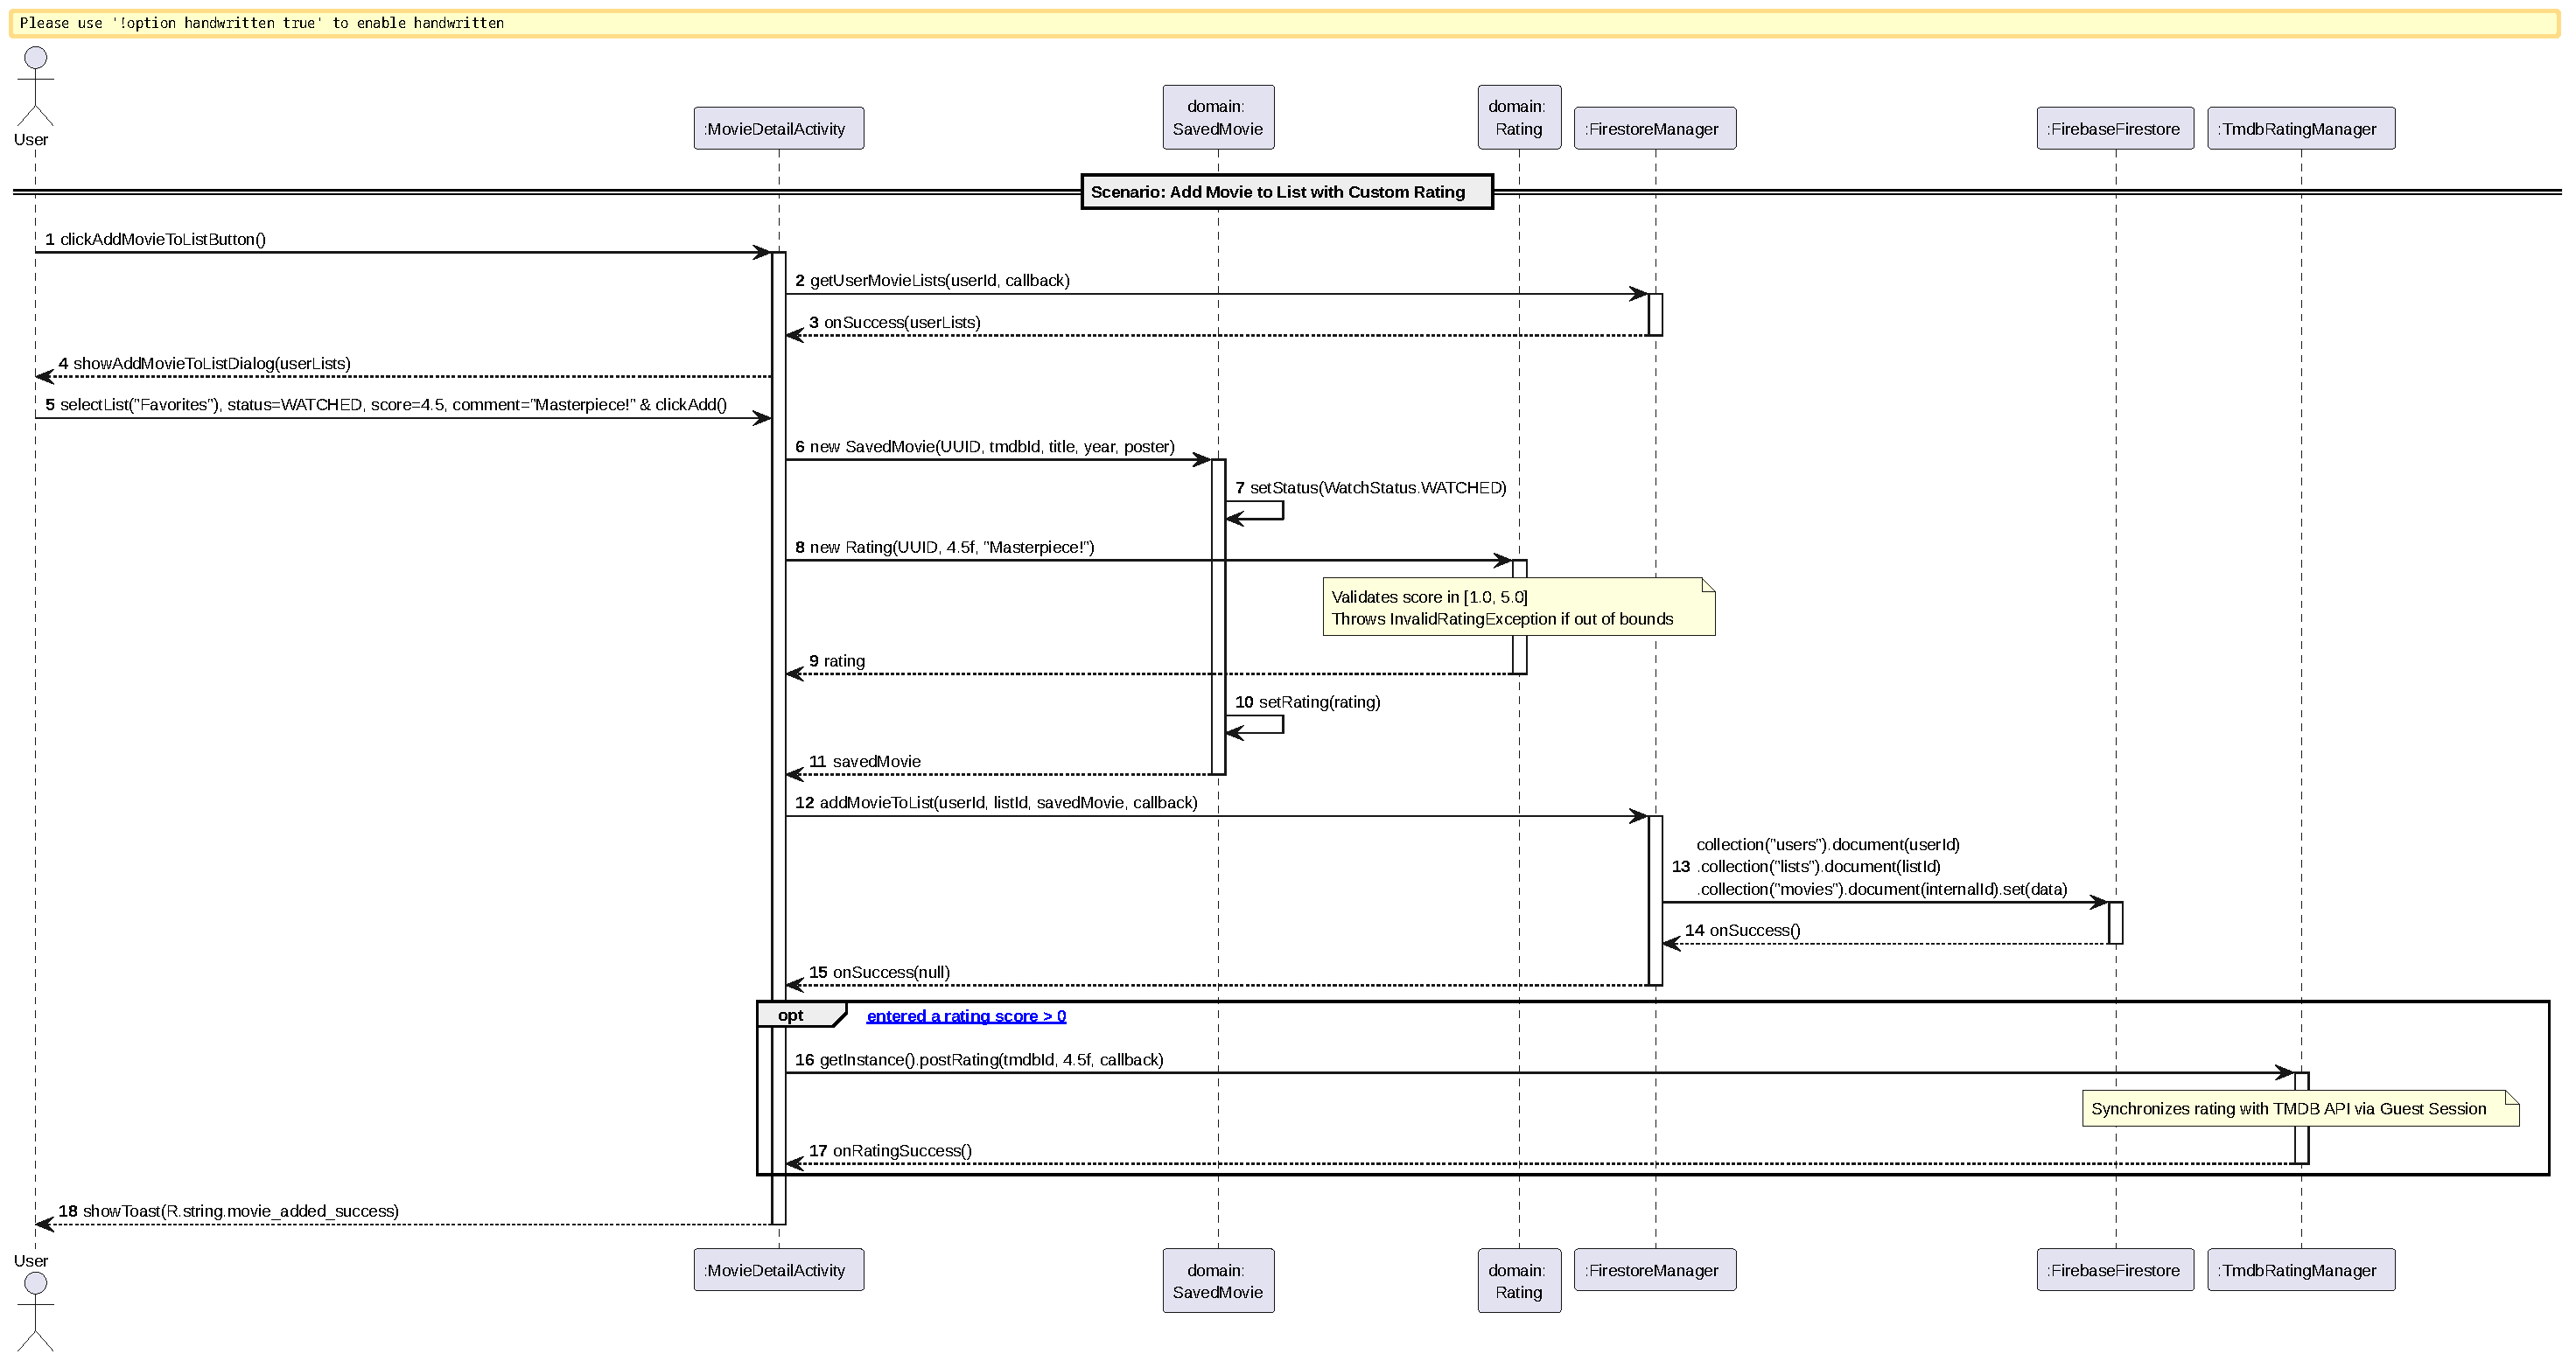
\includegraphics[width=0.85\textwidth]{figures/Use_Cases/UC3-SD.pdf}
    \caption{UC3: Add Movie and Rating Design Sequence Diagram}
    \label{fig:uc3-sd}
\end{figure}

\newpage

% --------------------------------------------------------------------
% UC4
% --------------------------------------------------------------------
\vspace{0.2cm}
\noindent{\Large \textbf{Use Case 4: Search Movies and Streaming Watch Providers}}
\vspace{0.2cm}

The specification for UC4 is detailed in Table \ref{tab:uc4}, and its execution flow is represented in Figure \ref{fig:uc4-sd}.

\begin{center}
    \small
    \captionof{table}{Use Case 4: Search TMDB and View Providers} \label{tab:uc4}
    \vspace{4pt}
    \begin{tabular}{@{}>{\raggedright\arraybackslash}p{2.8cm}
            >{\raggedright\arraybackslash}p{8.8cm}@{}}
        \hline
        \textbf{Actor}          & User \\
        \hline
        \textbf{Use case name}  & Search Movies and Streaming Watch Providers \\
        \textbf{Description}    & Allows the user to search the TMDB global catalog by title and inspect localized streaming providers (flatrate, rent, buy) in Portugal. \\
        \textbf{Precondition}   & Device connected to the Internet; TMDB API key configured. \\
        \textbf{Post-condition} & Movie search results displayed in RecyclerView; selecting a movie displays streaming platform logos. \\
        \textbf{Main flow}      & 
        1. User enters search keywords in MovieSearchActivity and taps search. \newline
        2. System reads default country preference ("PT") from SharedPrefManager. \newline
        3. Retrofit asynchronously dispatches non-blocking GET \texttt{/search/movie} request. \newline
        4. Results are mapped to DTOs and rendered with Glide poster loading. \newline
        5. User selects a movie; MovieDetailActivity loads localized watch providers. \newline
        6. System maps country providers to domain WatchProvider entities and renders logos. \\
        \textbf{Alternative path} & 
        If no movies match query, system presents empty state suggesting alternative keywords. \\
        \hline
    \end{tabular}
\end{center}

\begin{figure}[H]
    \centering
    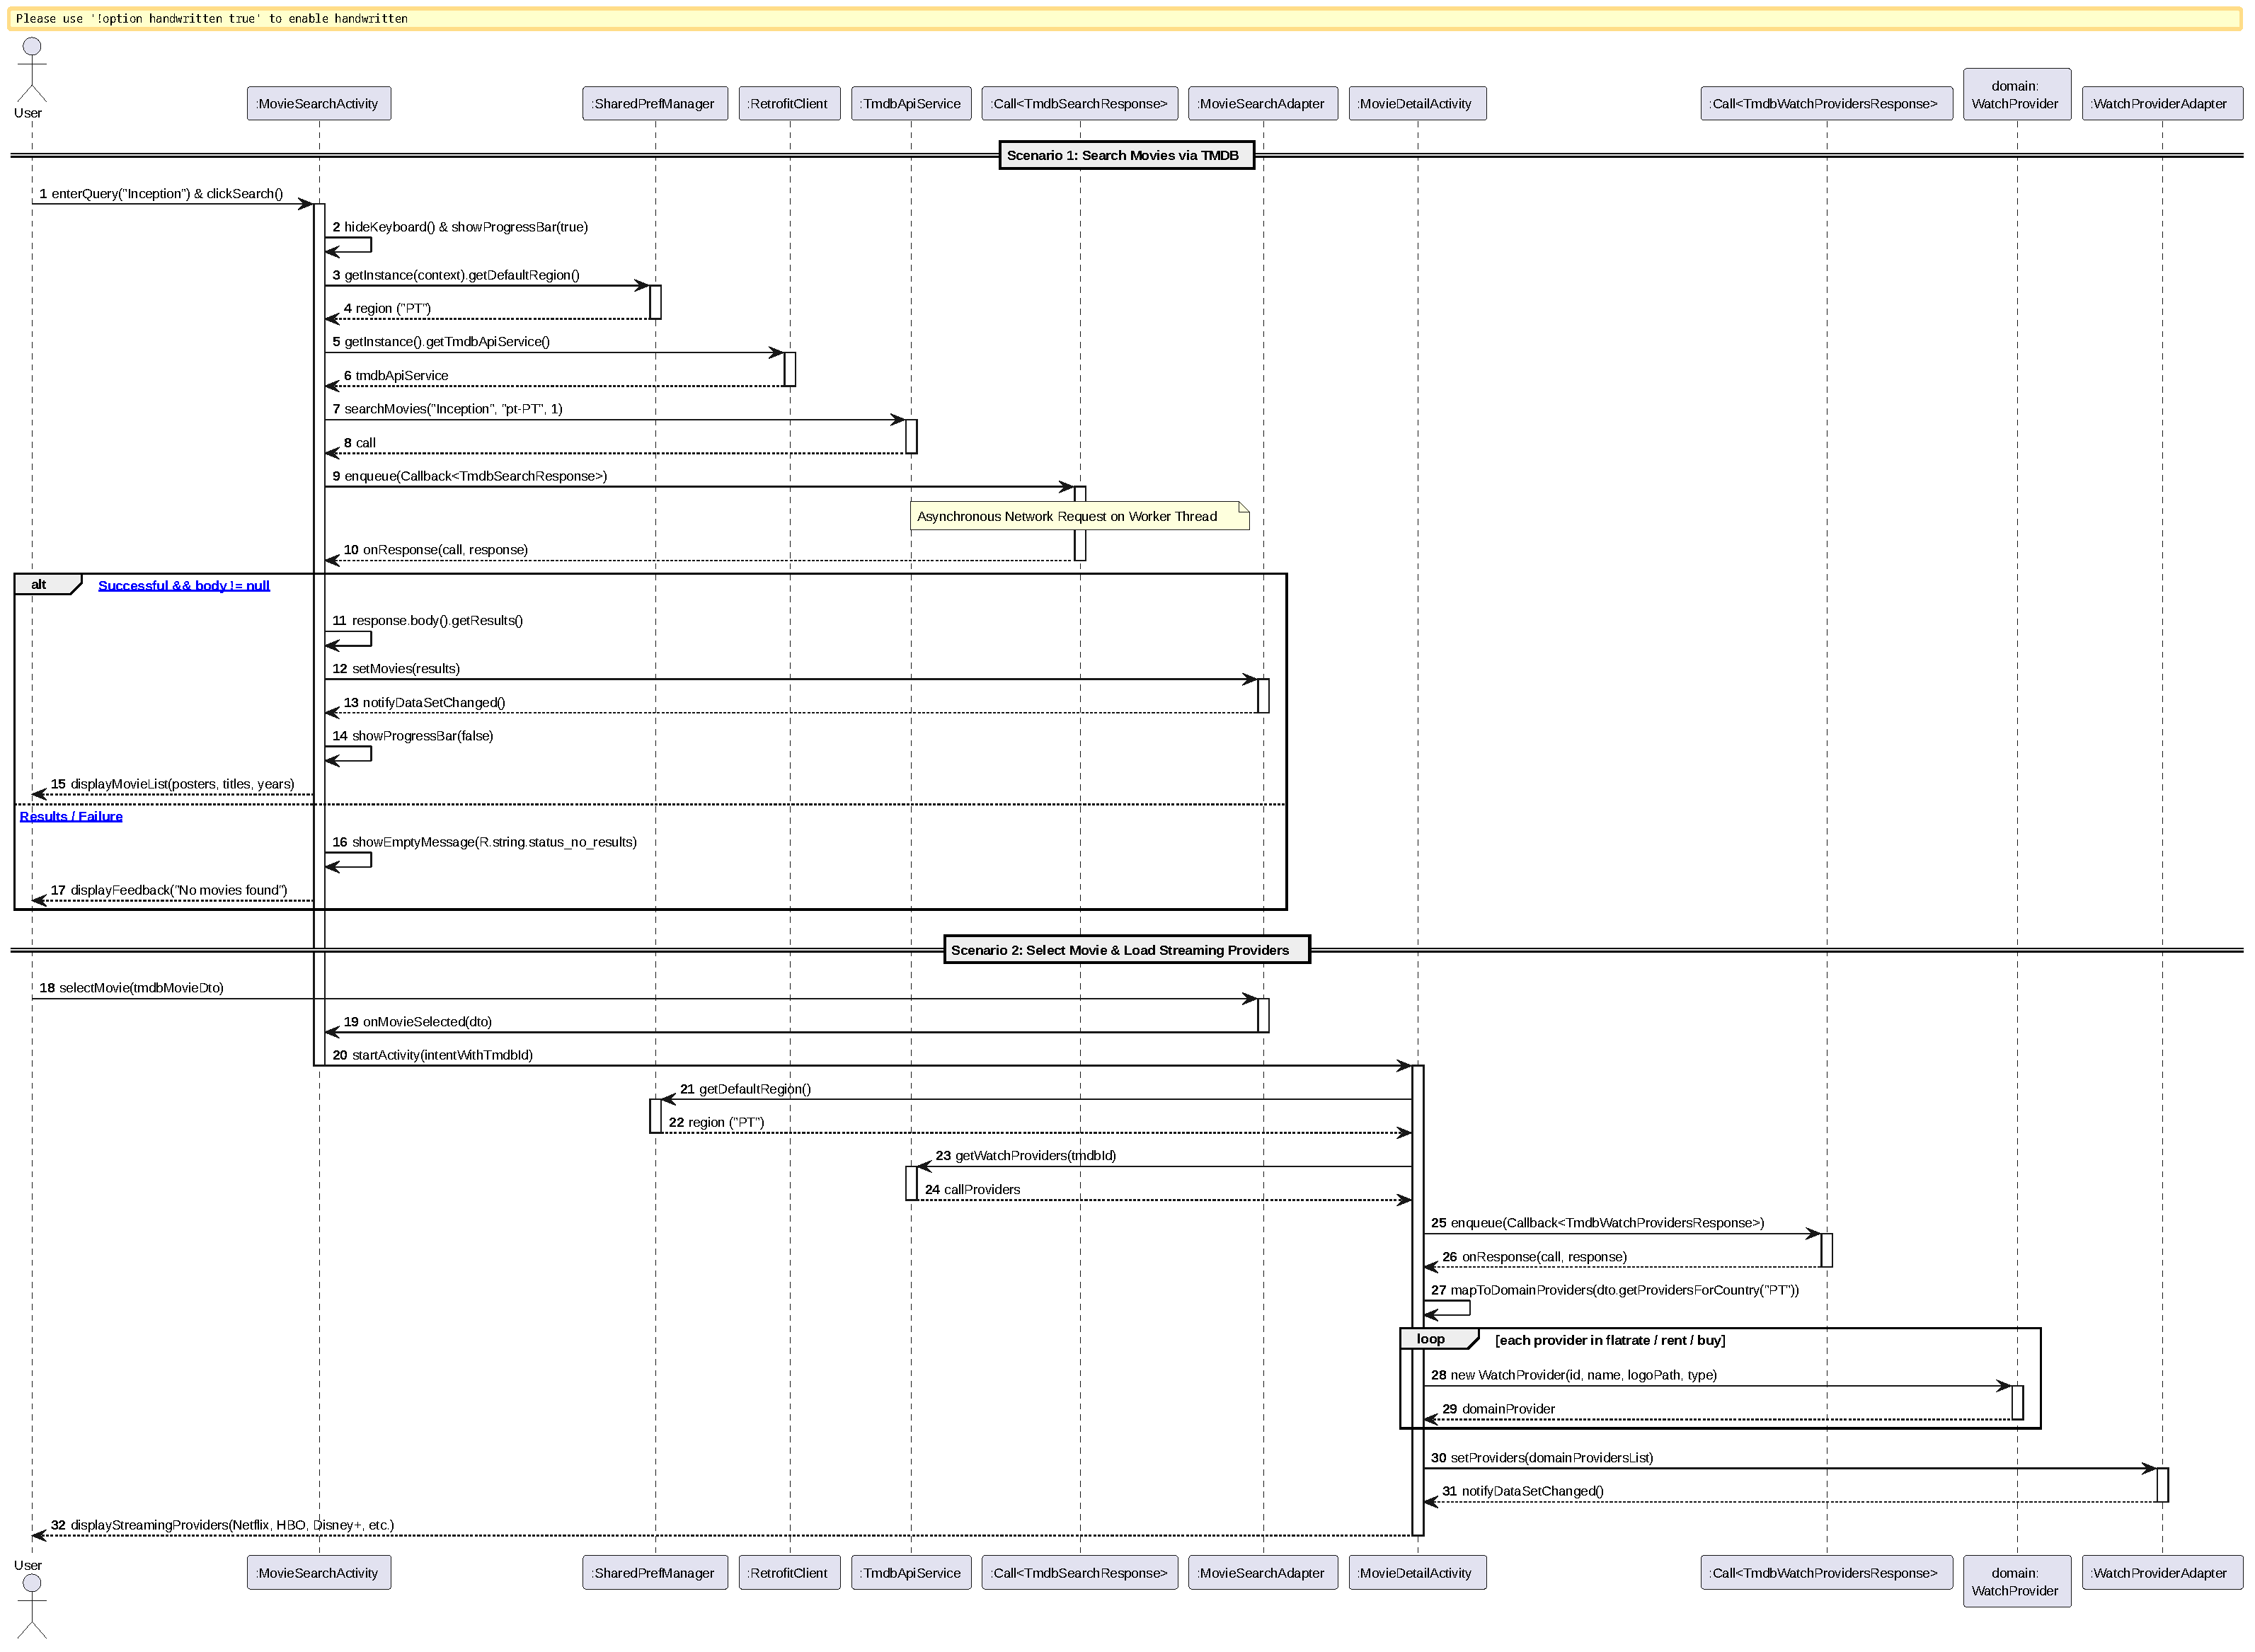
\includegraphics[width=0.85\textwidth]{figures/Use_Cases/UC4-SD.pdf}
    \caption{UC4: TMDB Search and Watch Providers Design Sequence Diagram}
    \label{fig:uc4-sd}
\end{figure}

\newpage

% --------------------------------------------------------------------
% UC5
% --------------------------------------------------------------------
\vspace{0.2cm}
\noindent{\Large \textbf{Use Case 5: Locate Nearby Cinemas (GPS + Foursquare + OSMDroid)}}
\vspace{0.2cm}

The specification for UC5 is detailed in Table \ref{tab:uc5}, and its execution flow is represented in Figure \ref{fig:uc5-sd}.

\begin{center}
    \small
    \captionof{table}{Use Case 5: Nearby Cinemas on Interactive Map} \label{tab:uc5}
    \vspace{4pt}
    \begin{tabular}{@{}>{\raggedright\arraybackslash}p{2.8cm}
            >{\raggedright\arraybackslash}p{8.8cm}@{}}
        \hline
        \textbf{Actor}          & User \\
        \hline
        \textbf{Use case name}  & Locate Nearby Cinemas \\
        \textbf{Description}    & Acquires device GPS coordinates, queries Foursquare Places API within user radius, and plots cinema markers with radius circumference on OSMDroid map. \\
        \textbf{Precondition}   & Location services enabled; runtime permission granted. \\
        \textbf{Post-condition} & Interactive map centered on GPS position with translucent radius circle and clickable cinema pins; turn-by-turn navigation launched on tap. \\
        \textbf{Main flow}      & 
        1. User opens CinemasActivity. \newline
        2. System checks \texttt{ACCESS\_FINE\_LOCATION}; requests permission if missing. \newline
        3. LocationHelper acquires device coordinates via native LocationManager. \newline
        4. System reads cinema radius from preferences, centers OSMDroid map, and draws a translucent blue radius polygon. \newline
        5. Retrofit queries Foursquare Places API (\texttt{category=10024}) with Bearer token. \newline
        6. Results mapped to pure Cinema domain entities; pins plotted with pop-up bubbles. \newline
        7. Tapping a pin or list item opens Google Maps navigation via \texttt{geo:} implicit intent. \\
        \textbf{Alternative path} & 
        If user denies location permission, an informative message is shown offering settings shortcut without crashing. \\
        \hline
    \end{tabular}
\end{center}

\begin{figure}[H]
    \centering
    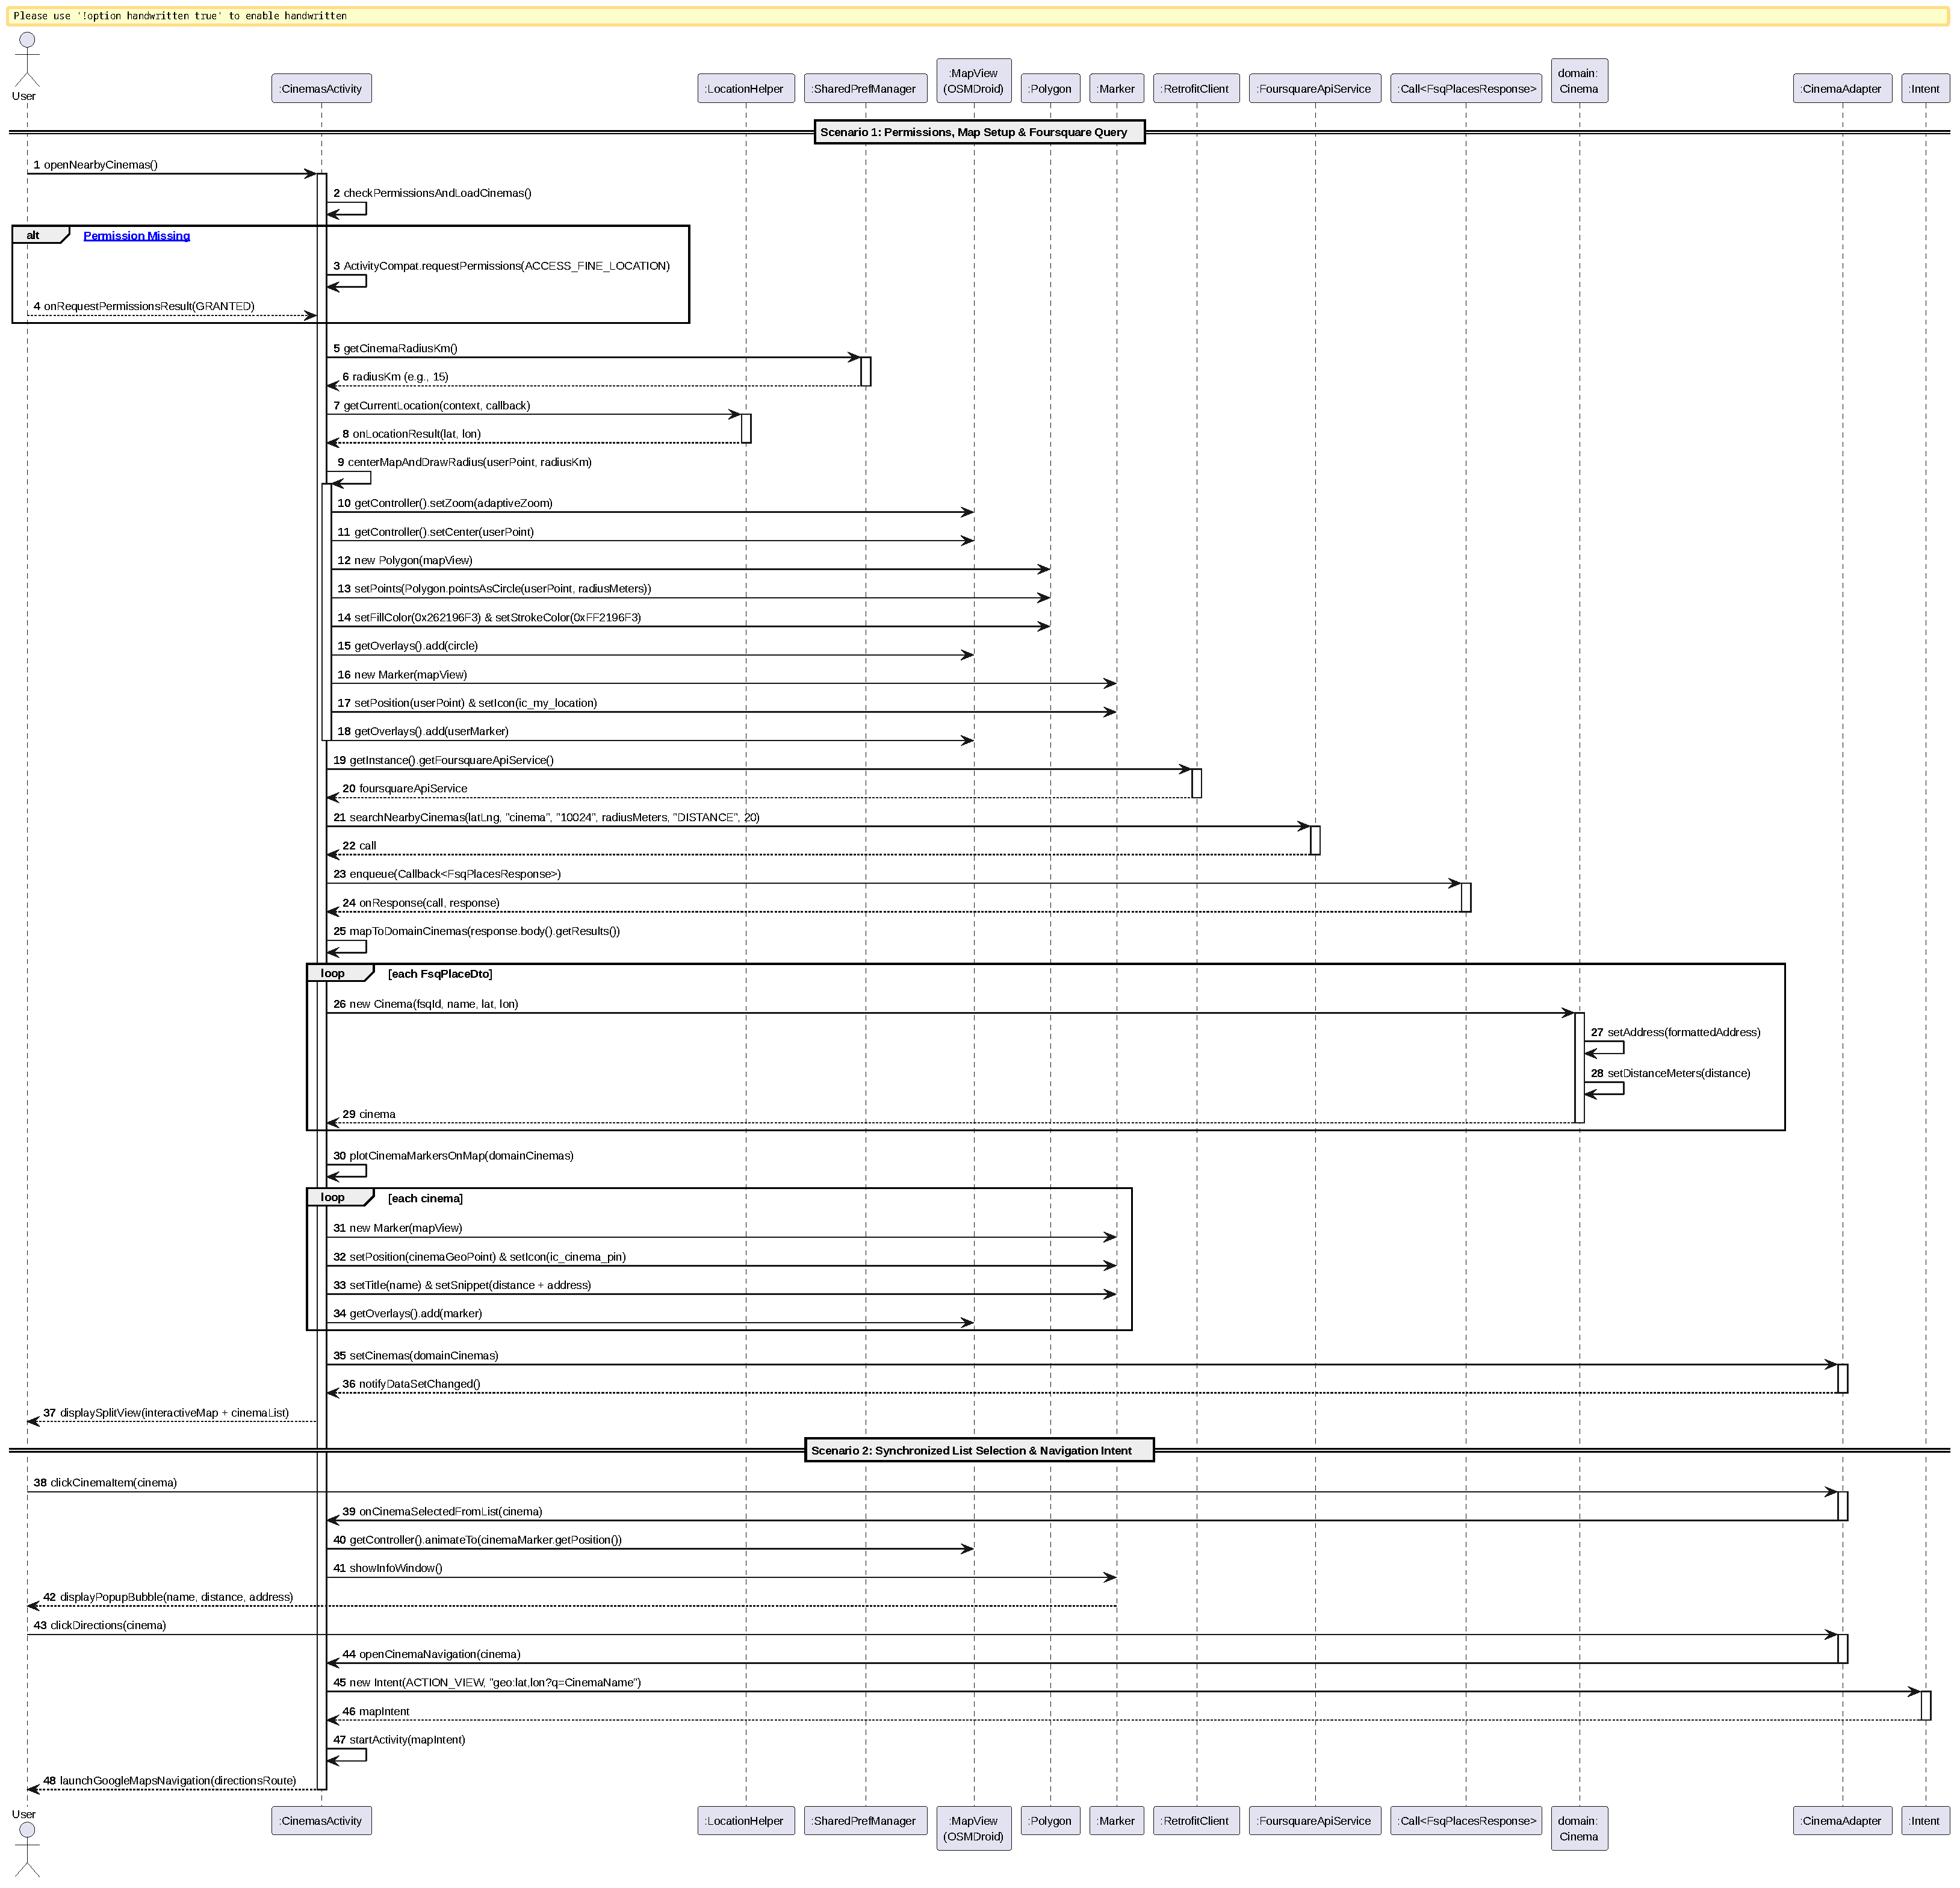
\includegraphics[width=0.85\textwidth]{figures/Use_Cases/UC5-SD.pdf}
    \caption{UC5: Nearby Cinemas and OSMDroid Map Design Sequence Diagram}
    \label{fig:uc5-sd}
\end{figure}

\newpage

% --------------------------------------------------------------------
% UC6
% --------------------------------------------------------------------
\vspace{0.2cm}
\noindent{\Large \textbf{Use Case 6: Shake to Suggest Recommendation (Accelerometer)}}
\vspace{0.2cm}

The specification for UC6 is detailed in Table \ref{tab:uc6}, and its execution flow is represented in Figure \ref{fig:uc6-sd}.

\begin{center}
    \small
    \captionof{table}{Use Case 6: Shake to Suggest} \label{tab:uc6}
    \vspace{4pt}
    \begin{tabular}{@{}>{\raggedright\arraybackslash}p{2.8cm}
            >{\raggedright\arraybackslash}p{8.8cm}@{}}
        \hline
        \textbf{Actor}          & User \\
        \hline
        \textbf{Use case name}  & Shake to Suggest \\
        \textbf{Description}    & Recommends a critically acclaimed movie matching the user's streaming subscriptions and minimum rating upon detecting a physical device shake. \\
        \textbf{Precondition}   & Device equipped with physical accelerometer; app in foreground. \\
        \textbf{Post-condition} & Device emits gentle haptic vibration and presents movie recommendation dialog without stacking multiple modals. \\
        \textbf{Main flow}      & 
        1. User vigorously shakes the physical phone. \newline
        2. ShakeDetector computes vectorial acceleration; verifies multi-peak threshold ($>2.7g$). \newline
        3. MainActivity triggers haptic pulse via Vibrator service. \newline
        4. System queries background recommendation cache matching user preference filters. \newline
        5. Recommendation dialog displays movie poster, score, synopsis, and action buttons. \newline
        6. User can tap "View Details" to open movie page or "Shake Again" to reshuffle. \\
        \textbf{Alternative path} & 
        If all cached recommendations were viewed, system queries the next TMDB discover page asynchronously. \\
        \hline
    \end{tabular}
\end{center}

\begin{figure}[H]
    \centering
    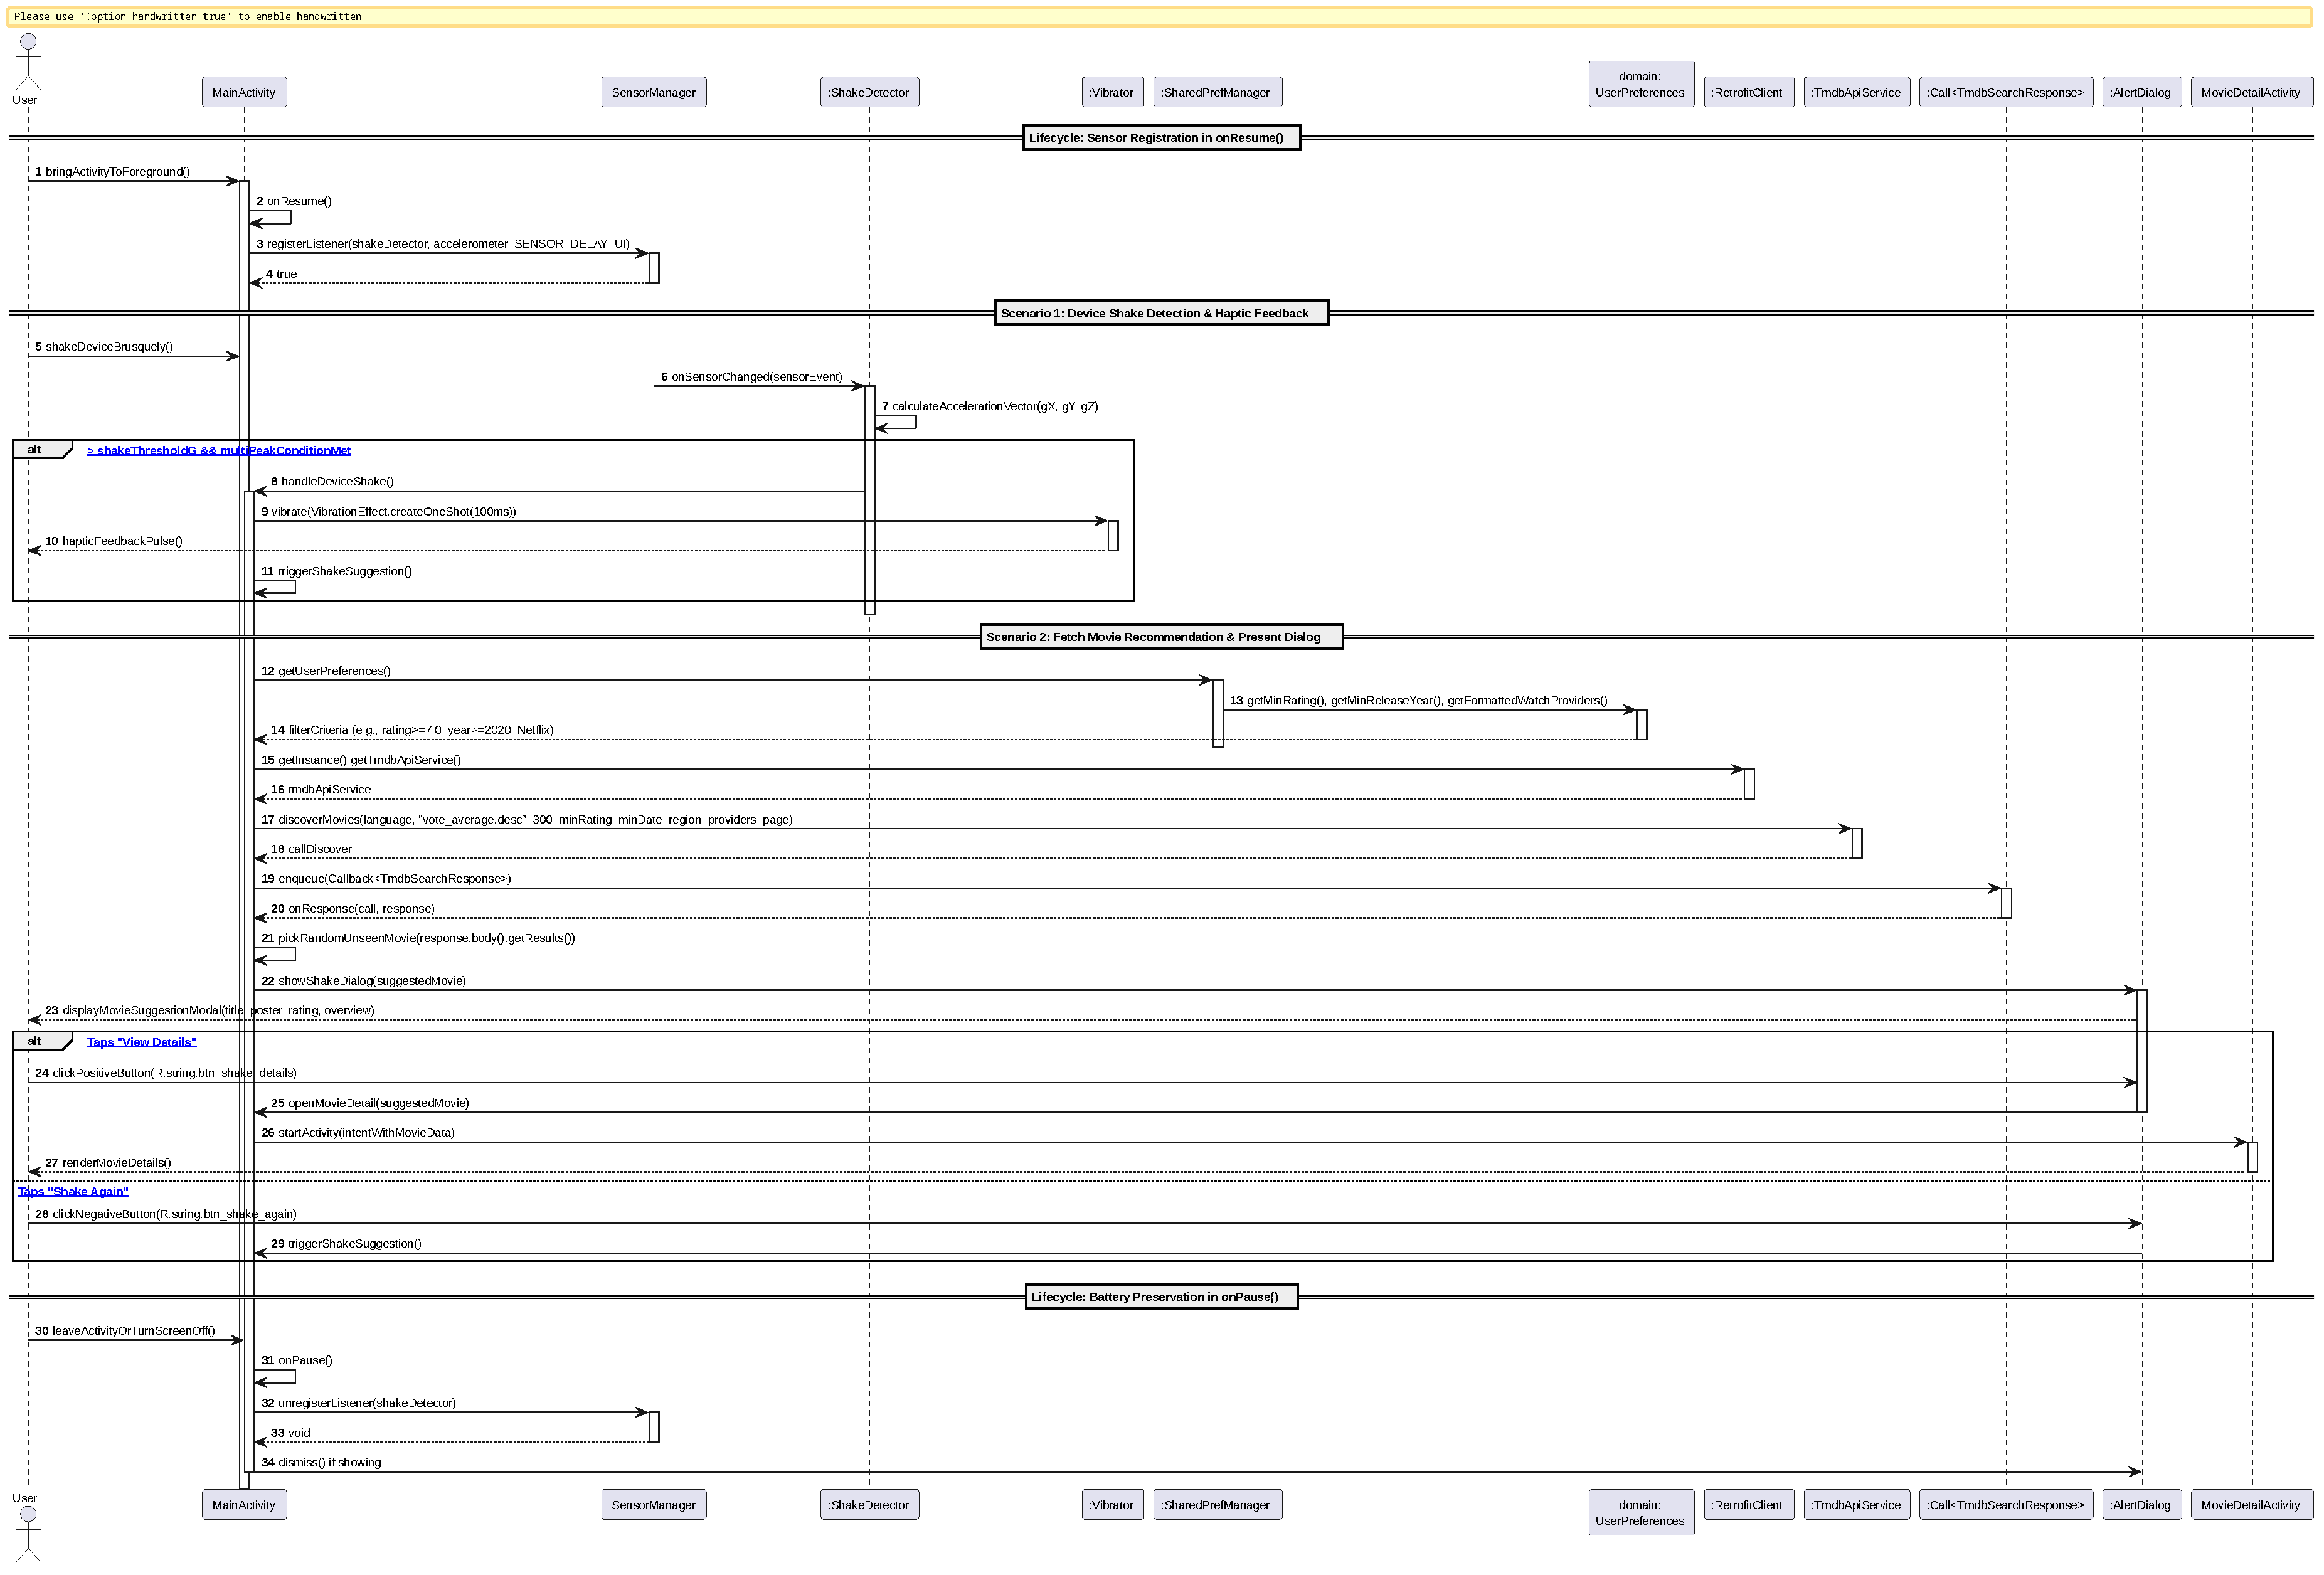
\includegraphics[width=0.85\textwidth]{figures/Use_Cases/UC6-SD.pdf}
    \caption{UC6: Shake to Suggest Design Sequence Diagram}
    \label{fig:uc6-sd}
\end{figure}

\newpage

% --------------------------------------------------------------------
% UC7
% --------------------------------------------------------------------
\vspace{0.2cm}
\noindent{\Large \textbf{Use Case 7: User Profile and Session Logout}}
\vspace{0.2cm}

The specification for UC7 is detailed in Table \ref{tab:uc7}, and its execution flow is represented in Figure \ref{fig:uc7-sd}.

\begin{center}
    \small
    \captionof{table}{Use Case 7: User Profile and Logout} \label{tab:uc7}
    \vspace{4pt}
    \begin{tabular}{@{}>{\raggedright\arraybackslash}p{2.8cm}
            >{\raggedright\arraybackslash}p{8.8cm}@{}}
        \hline
        \textbf{Actor}          & Authenticated User \\
        \hline
        \textbf{Use case name}  & User Profile and Session Logout \\
        \textbf{Description}    & Displays account metadata (email, registration date, total personal lists) and provides secure session termination. \\
        \textbf{Precondition}   & Active user session. \\
        \textbf{Post-condition} & Firebase session terminated; user navigated to LoginActivity with cleared task stack. \\
        \textbf{Main flow}      & 
        1. User selects the "Profile" destination in bottom navigation. \newline
        2. ProfileActivity queries FirebaseUser metadata and Firestore list counts. \newline
        3. User inspects account summary and taps "Log Out". \newline
        4. System displays confirmation dialog. \newline
        5. User confirms; FirebaseAuthManager invokes \texttt{signOut()}. \newline
        6. System clears activity backstack and redirects to LoginActivity. \\
        \textbf{Alternative path} & 
        If user cancels the logout prompt, the dialog dismisses and session remains active. \\
        \hline
    \end{tabular}
\end{center}

\begin{figure}[H]
    \centering
    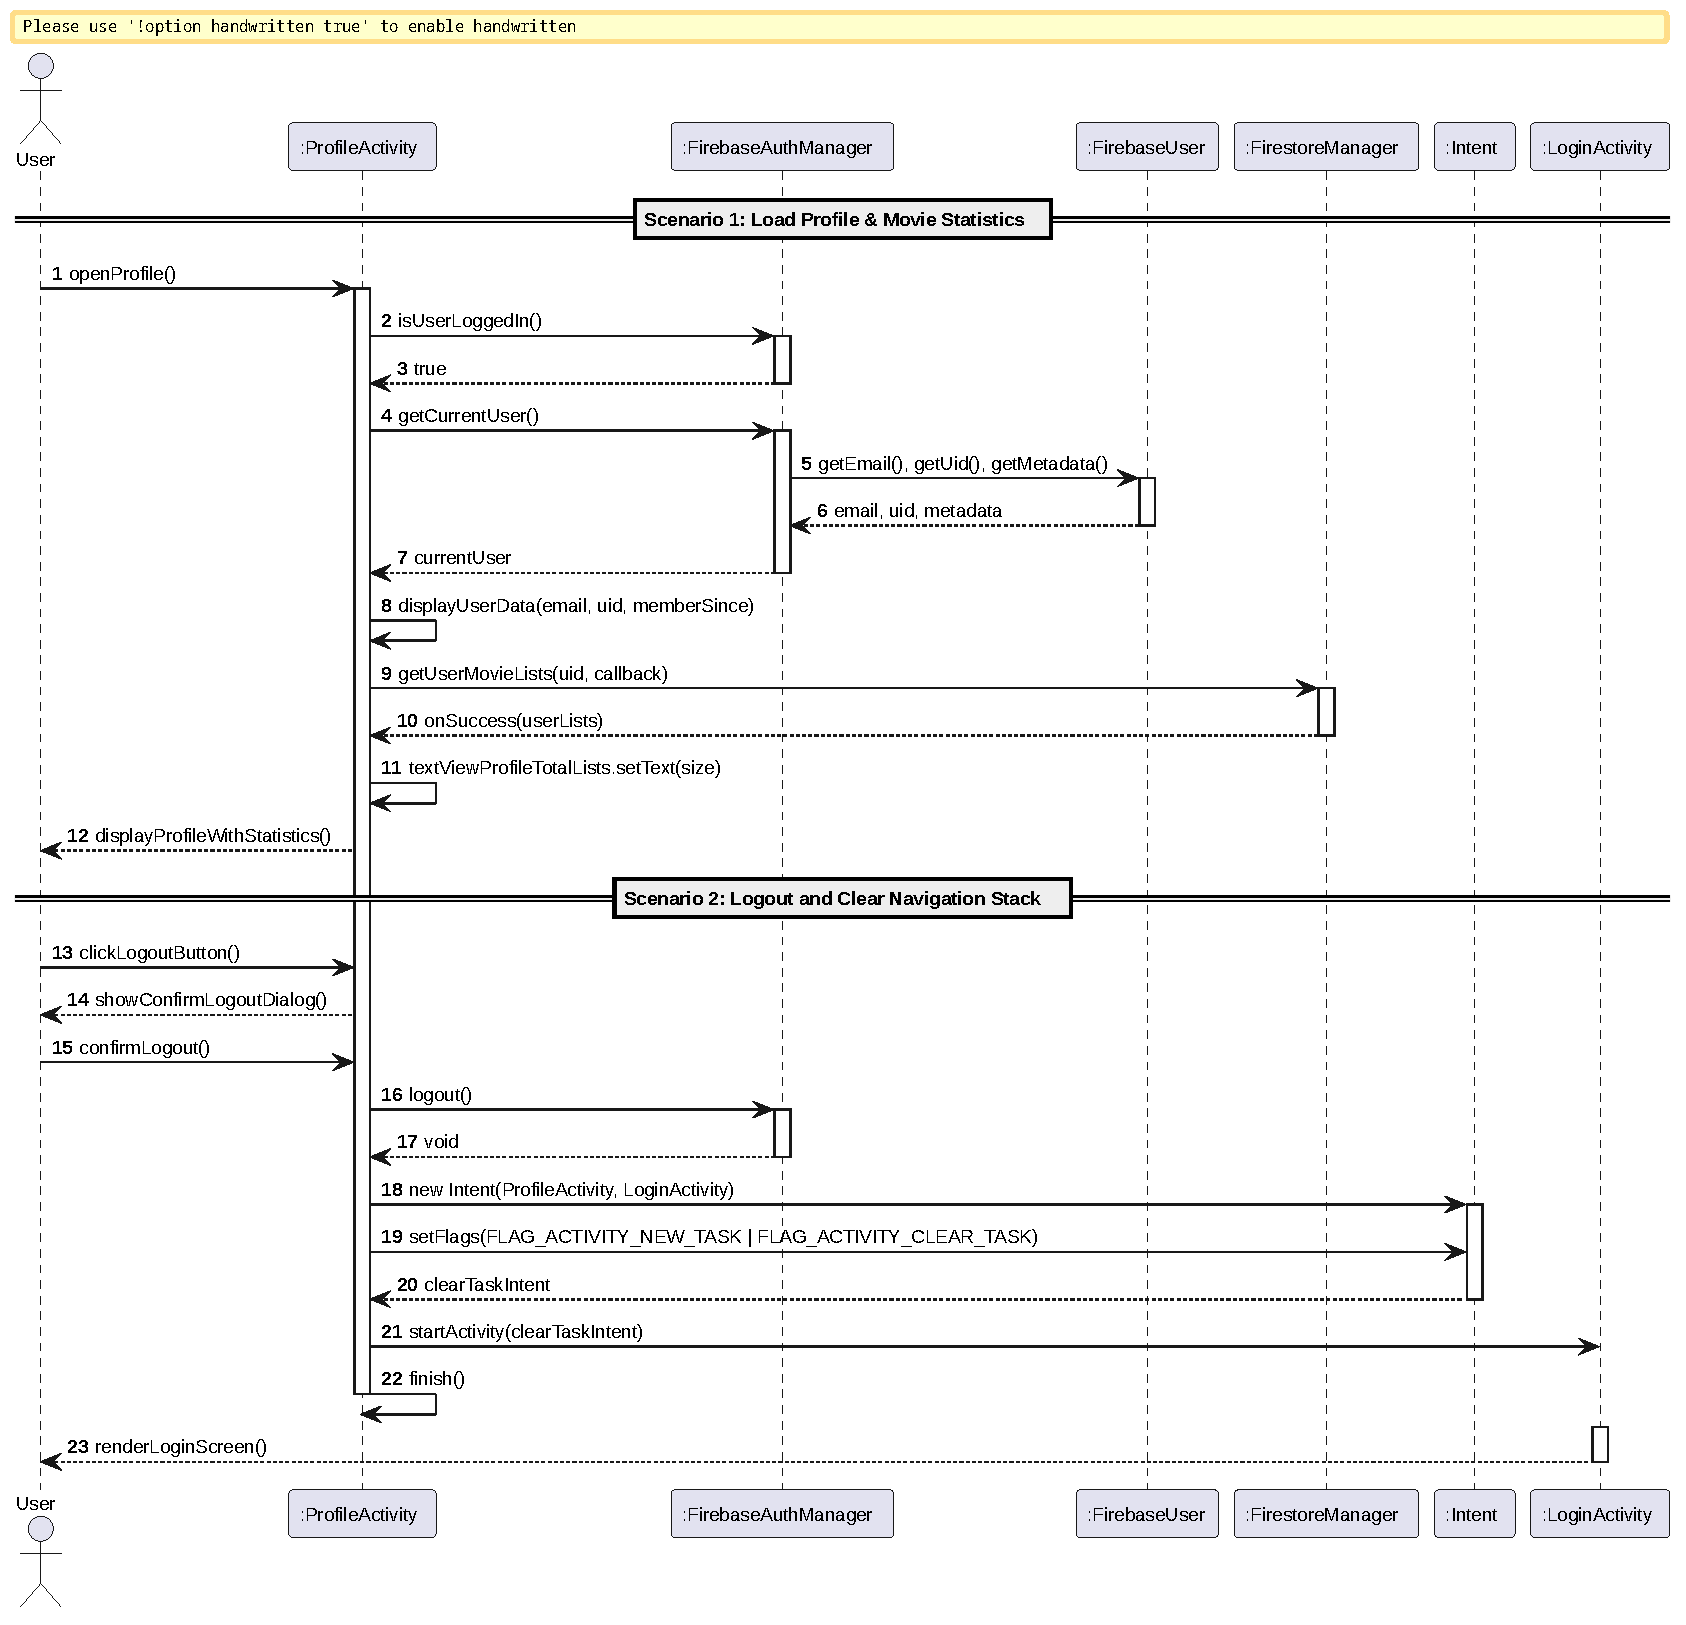
\includegraphics[width=0.85\textwidth]{figures/Use_Cases/UC7-SD.pdf}
    \caption{UC7: Profile and Logout Design Sequence Diagram}
    \label{fig:uc7-sd}
\end{figure}

\newpage

% --------------------------------------------------------------------
% UC8
% --------------------------------------------------------------------
\vspace{0.2cm}
\noindent{\Large \textbf{Use Case 8: Configure Local Preferences (SharedPreferences)}}
\vspace{0.2cm}

The specification for UC8 is detailed in Table \ref{tab:uc8}, and its execution flow is represented in Figure \ref{fig:uc8-sd}.

\begin{center}
    \small
    \captionof{table}{Use Case 8: Configure Local Preferences} \label{tab:uc8}
    \vspace{4pt}
    \begin{tabular}{@{}>{\raggedright\arraybackslash}p{2.8cm}
            >{\raggedright\arraybackslash}p{8.8cm}@{}}
        \hline
        \textbf{Actor}          & User \\
        \hline
        \textbf{Use case name}  & Configure Local Preferences \\
        \textbf{Description}    & Allows user to configure cinema search radius, default streaming country, shake sensitivity, and streaming subscriptions. \\
        \textbf{Precondition}   & None. \\
        \textbf{Post-condition} & UserPreferences updated and saved to SharedPreferences asynchronously via \texttt{.apply()}. \\
        \textbf{Main flow}      & 
        1. User taps the settings gear icon in the top toolbar. \newline
        2. System displays preferences modal prepopulated with current settings. \newline
        3. User updates parameters (e.g., radius=25km, threshold=2.7g, Netflix). \newline
        4. System instantiates UserPreferences domain entity and validates ranges. \newline
        5. SharedPrefManager invokes \texttt{editor.apply()} asynchronously. \newline
        6. ShakeDetector threshold updated and recommendation pool refreshed. \\
        \textbf{Alternative path} & 
        If numerical format is invalid, toast prompts user to correct input before saving. \\
        \hline
    \end{tabular}
\end{center}

\begin{figure}[H]
    \centering
    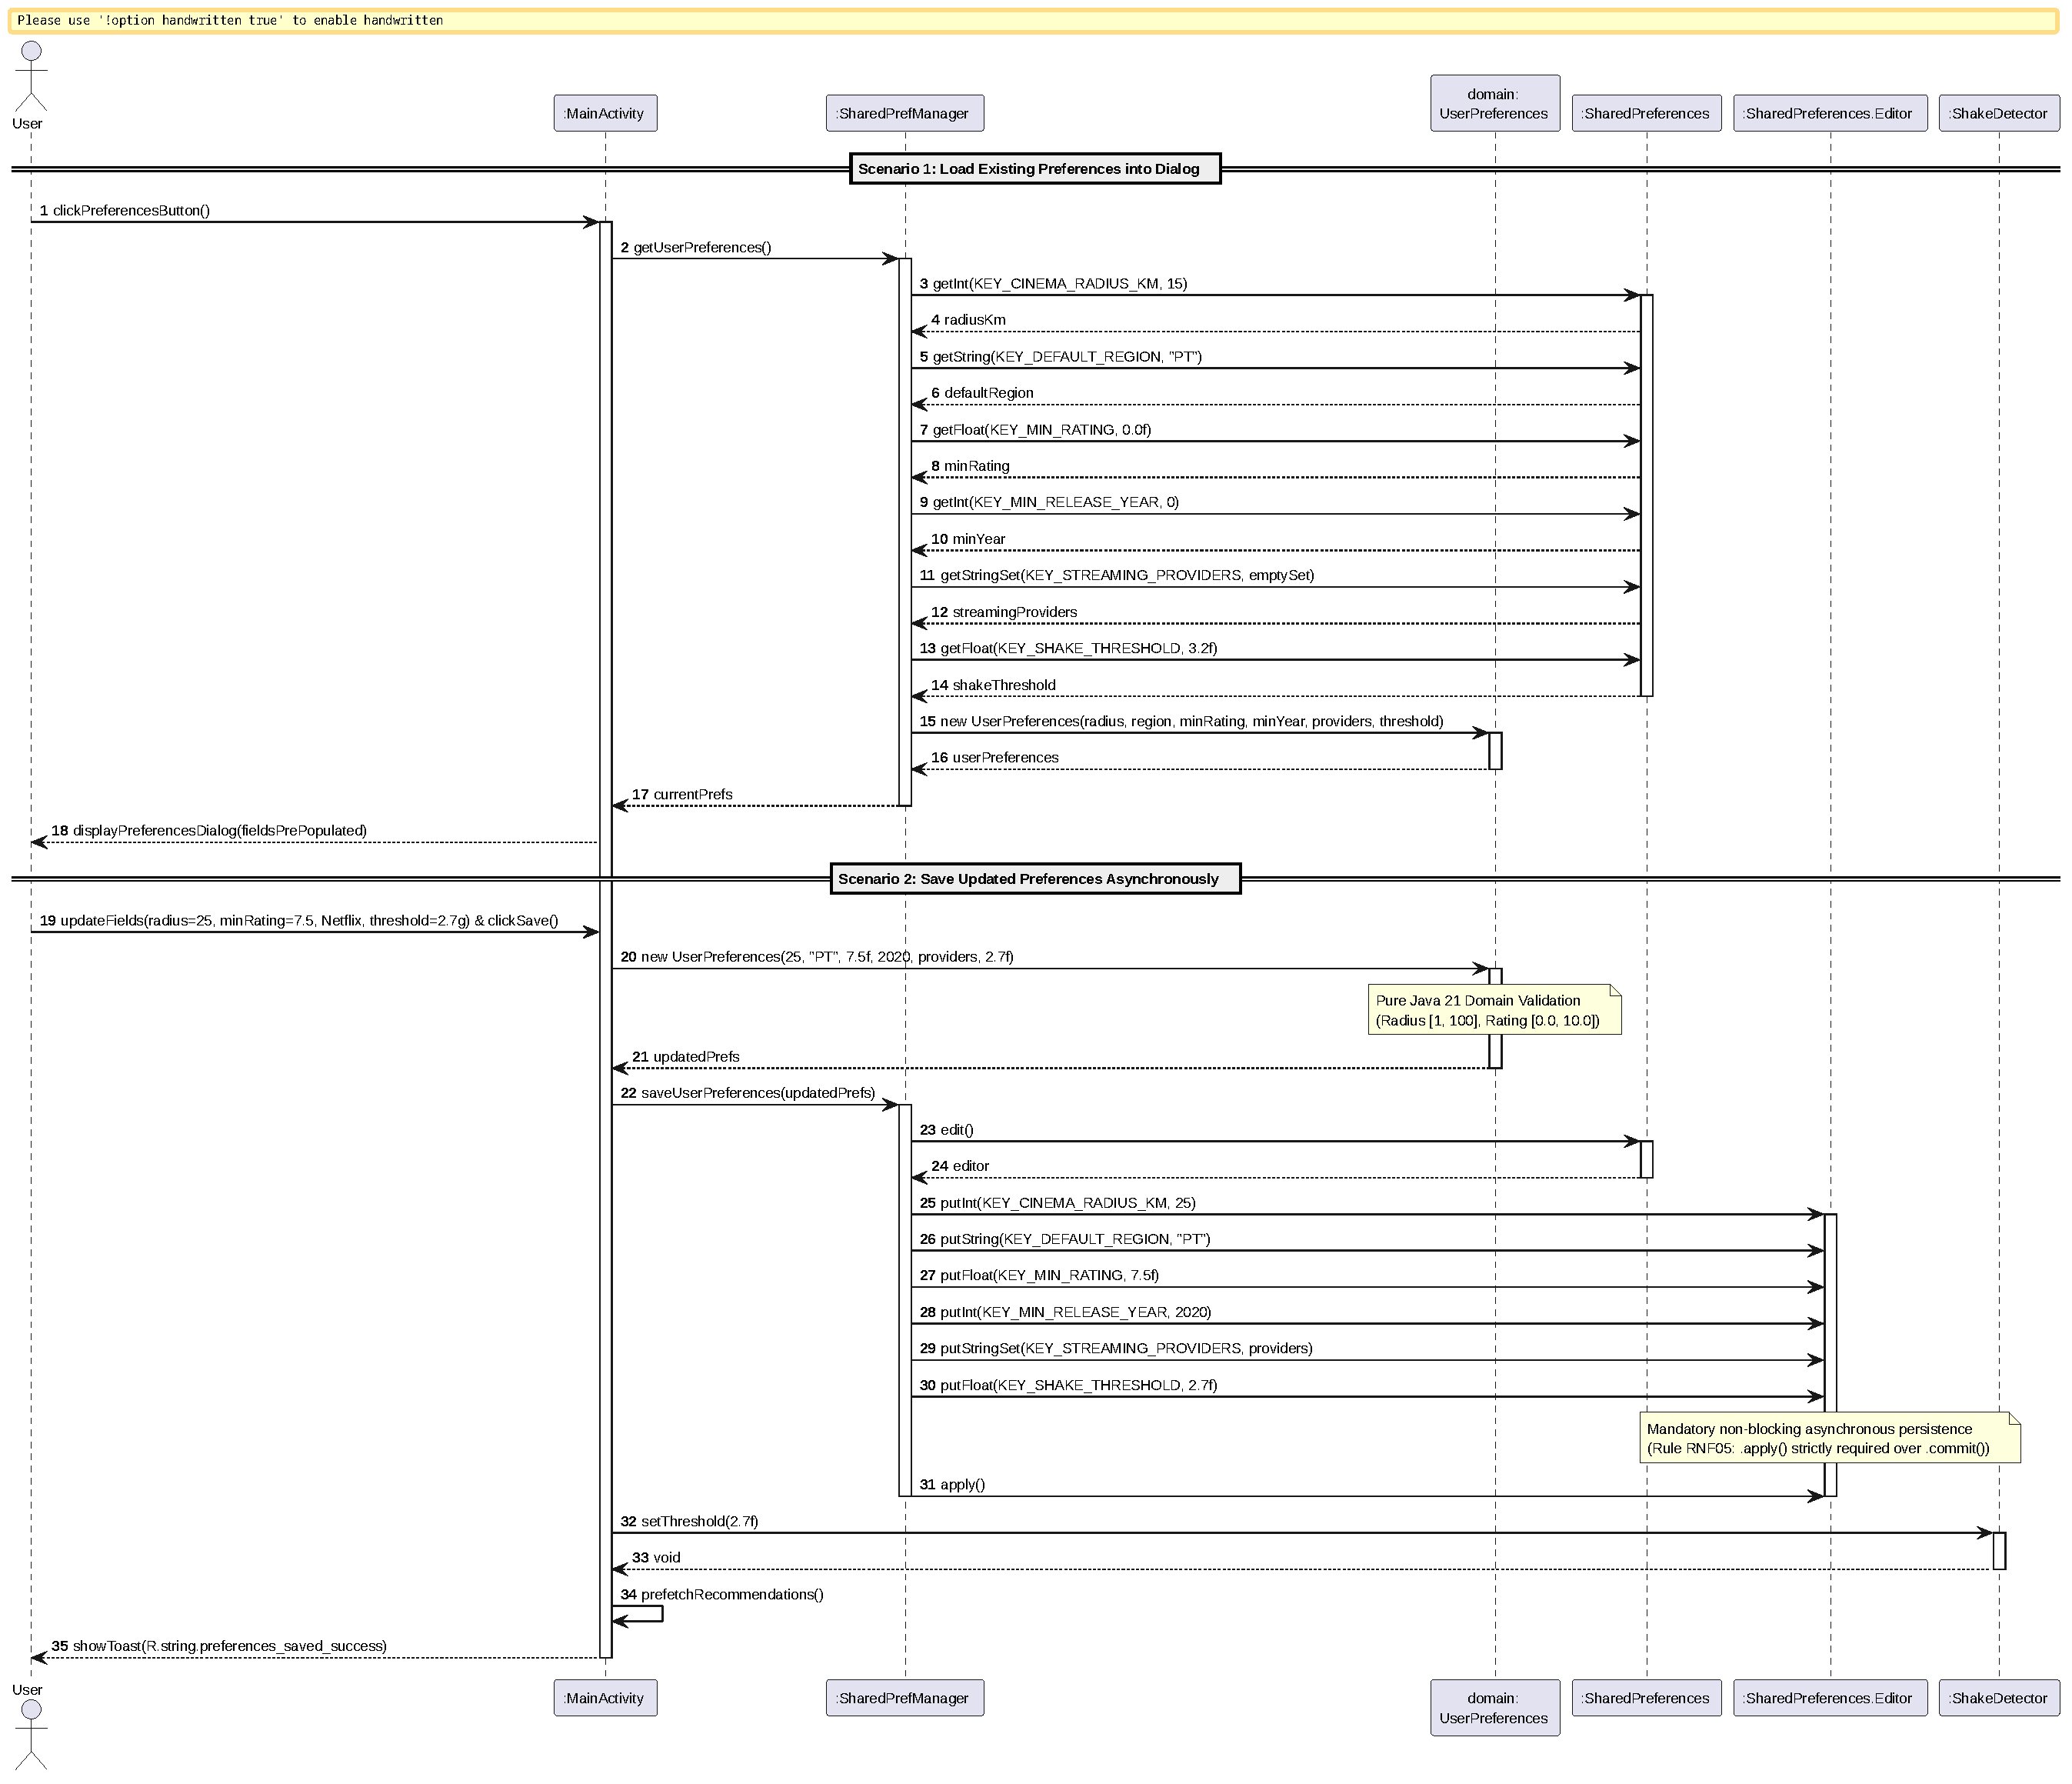
\includegraphics[width=0.85\textwidth]{figures/Use_Cases/UC8-SD.pdf}
    \caption{UC8: Local Preferences Design Sequence Diagram}
    \label{fig:uc8-sd}
\end{figure}

\newpage

% --------------------------------------------------------------------
% UC9
% --------------------------------------------------------------------
\vspace{0.2cm}
\noindent{\Large \textbf{Use Case 9: Filter and Sort Local Movie Collection}}
\vspace{0.2cm}

The specification for UC9 is detailed in Table \ref{tab:uc9}, and its execution flow is represented in Figure \ref{fig:uc9-sd}.

\begin{center}
    \small
    \captionof{table}{Use Case 9: Filter and Sort Collection} \label{tab:uc9}
    \vspace{4pt}
    \begin{tabular}{@{}>{\raggedright\arraybackslash}p{2.8cm}
            >{\raggedright\arraybackslash}p{8.8cm}@{}}
        \hline
        \textbf{Actor}          & User \\
        \hline
        \textbf{Use case name}  & Filter and Sort Collection \\
        \textbf{Description}    & Allows filtering saved movies by WatchStatus or search query, and sorting by title, rating, or release year using pure Java 21 comparators. \\
        \textbf{Precondition}   & List contains saved movies. \\
        \textbf{Post-condition} & RecyclerView updates displayed order and subset without blocking UI Thread. \\
        \textbf{Main flow}      & 
        1. User opens ListDetailsActivity. \newline
        2. User selects filter (e.g., status=WATCHED) or sort criterion (e.g., RATING\_DESC). \newline
        3. Activity delegates collection to \texttt{SavedMovieFilterSorter.filterAndSort()}. \newline
        4. Pure Java~21 \texttt{Comparator} chain executes sorting logic. \newline
        5. Adapter receives filtered list and calls \texttt{notifyDataSetChanged()}. \\
        \textbf{Alternative path} & 
        If no movies match filter, empty search notice is rendered. \\
        \hline
    \end{tabular}
\end{center}

\begin{figure}[H]
    \centering
    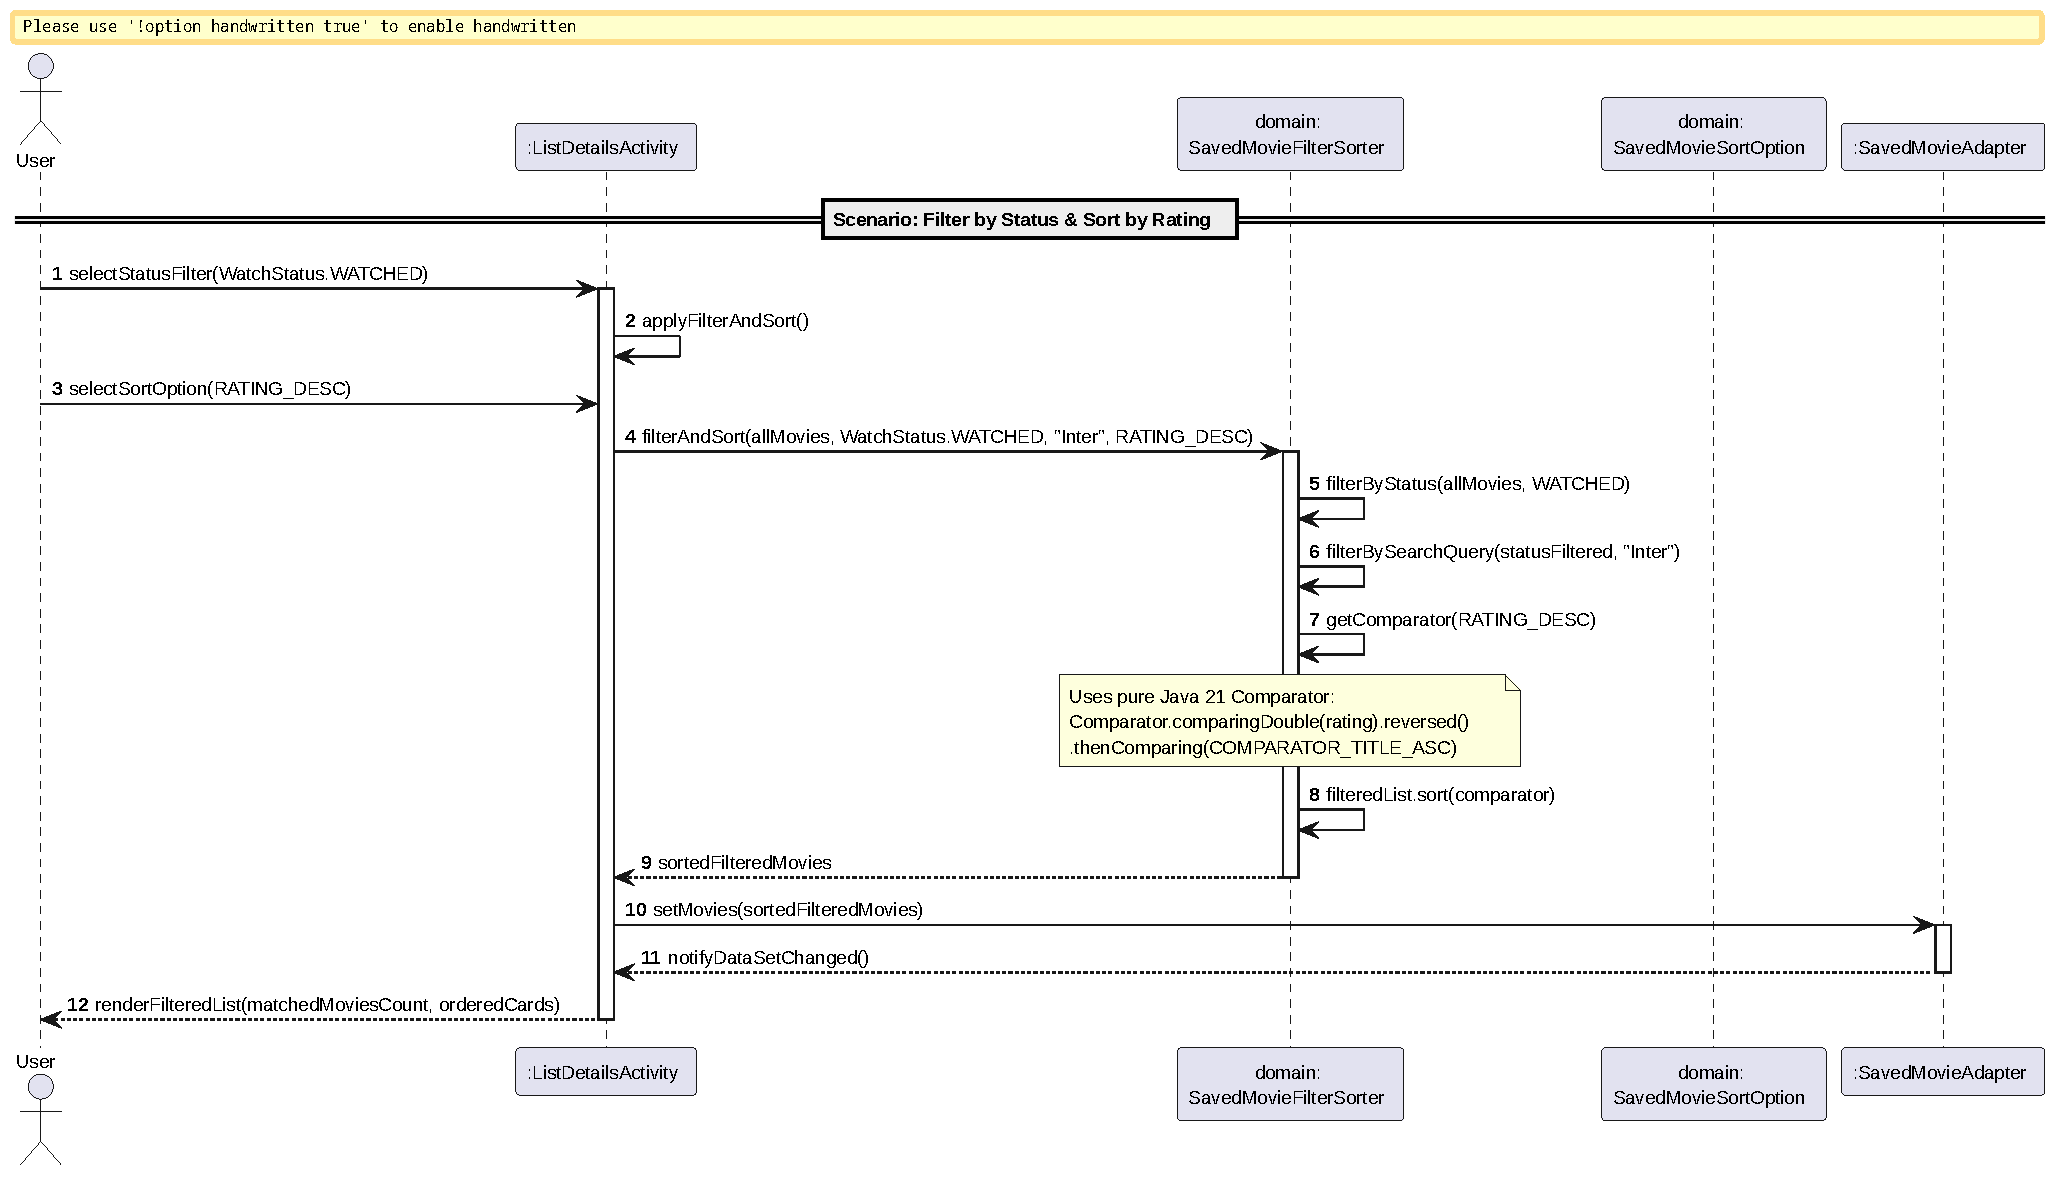
\includegraphics[width=0.85\textwidth]{figures/Use_Cases/UC9-SD.pdf}
    \caption{UC9: Collection Filter and Sort Design Sequence Diagram}
    \label{fig:uc9-sd}
\end{figure}

\newpage

% --------------------------------------------------------------------
% UC10
% --------------------------------------------------------------------
\vspace{0.2cm}
\noindent{\Large \textbf{Use Case 10: Play Official YouTube Video Trailers}}
\vspace{0.2cm}

The specification for UC10 is detailed in Table \ref{tab:uc10}, and its execution flow is represented in Figure \ref{fig:uc10-sd}.

\begin{center}
    \small
    \captionof{table}{Use Case 10: Play Official Trailers} \label{tab:uc10}
    \vspace{4pt}
    \begin{tabular}{@{}>{\raggedright\arraybackslash}p{2.8cm}
            >{\raggedright\arraybackslash}p{8.8cm}@{}}
        \hline
        \textbf{Actor}          & User \\
        \hline
        \textbf{Use case name}  & Play Official YouTube Trailers \\
        \textbf{Description}    & Queries TMDB for official YouTube trailer keys and launches video playback via native app intent with defensive web browser fallback. \\
        \textbf{Precondition}   & Internet connectivity available. \\
        \textbf{Post-condition} & Official trailer plays in YouTube app or web browser. \\
        \textbf{Main flow}      & 
        1. User taps "Watch Trailer" in MovieDetailActivity. \newline
        2. System disables button and queries GET \texttt{/movie/\{id\}/videos} via Retrofit. \newline
        3. Response parsed to identify official YouTube trailer key. \newline
        4. System fires implicit intent with URI \texttt{vnd.youtube:<key>}. \newline
        5. YouTube native app launches and begins video playback. \\
        \textbf{Alternative path} & 
        If YouTube app is not installed, \texttt{ActivityNotFoundException} is caught and URL opened in web browser. \\
        \hline
    \end{tabular}
\end{center}

\begin{figure}[H]
    \centering
    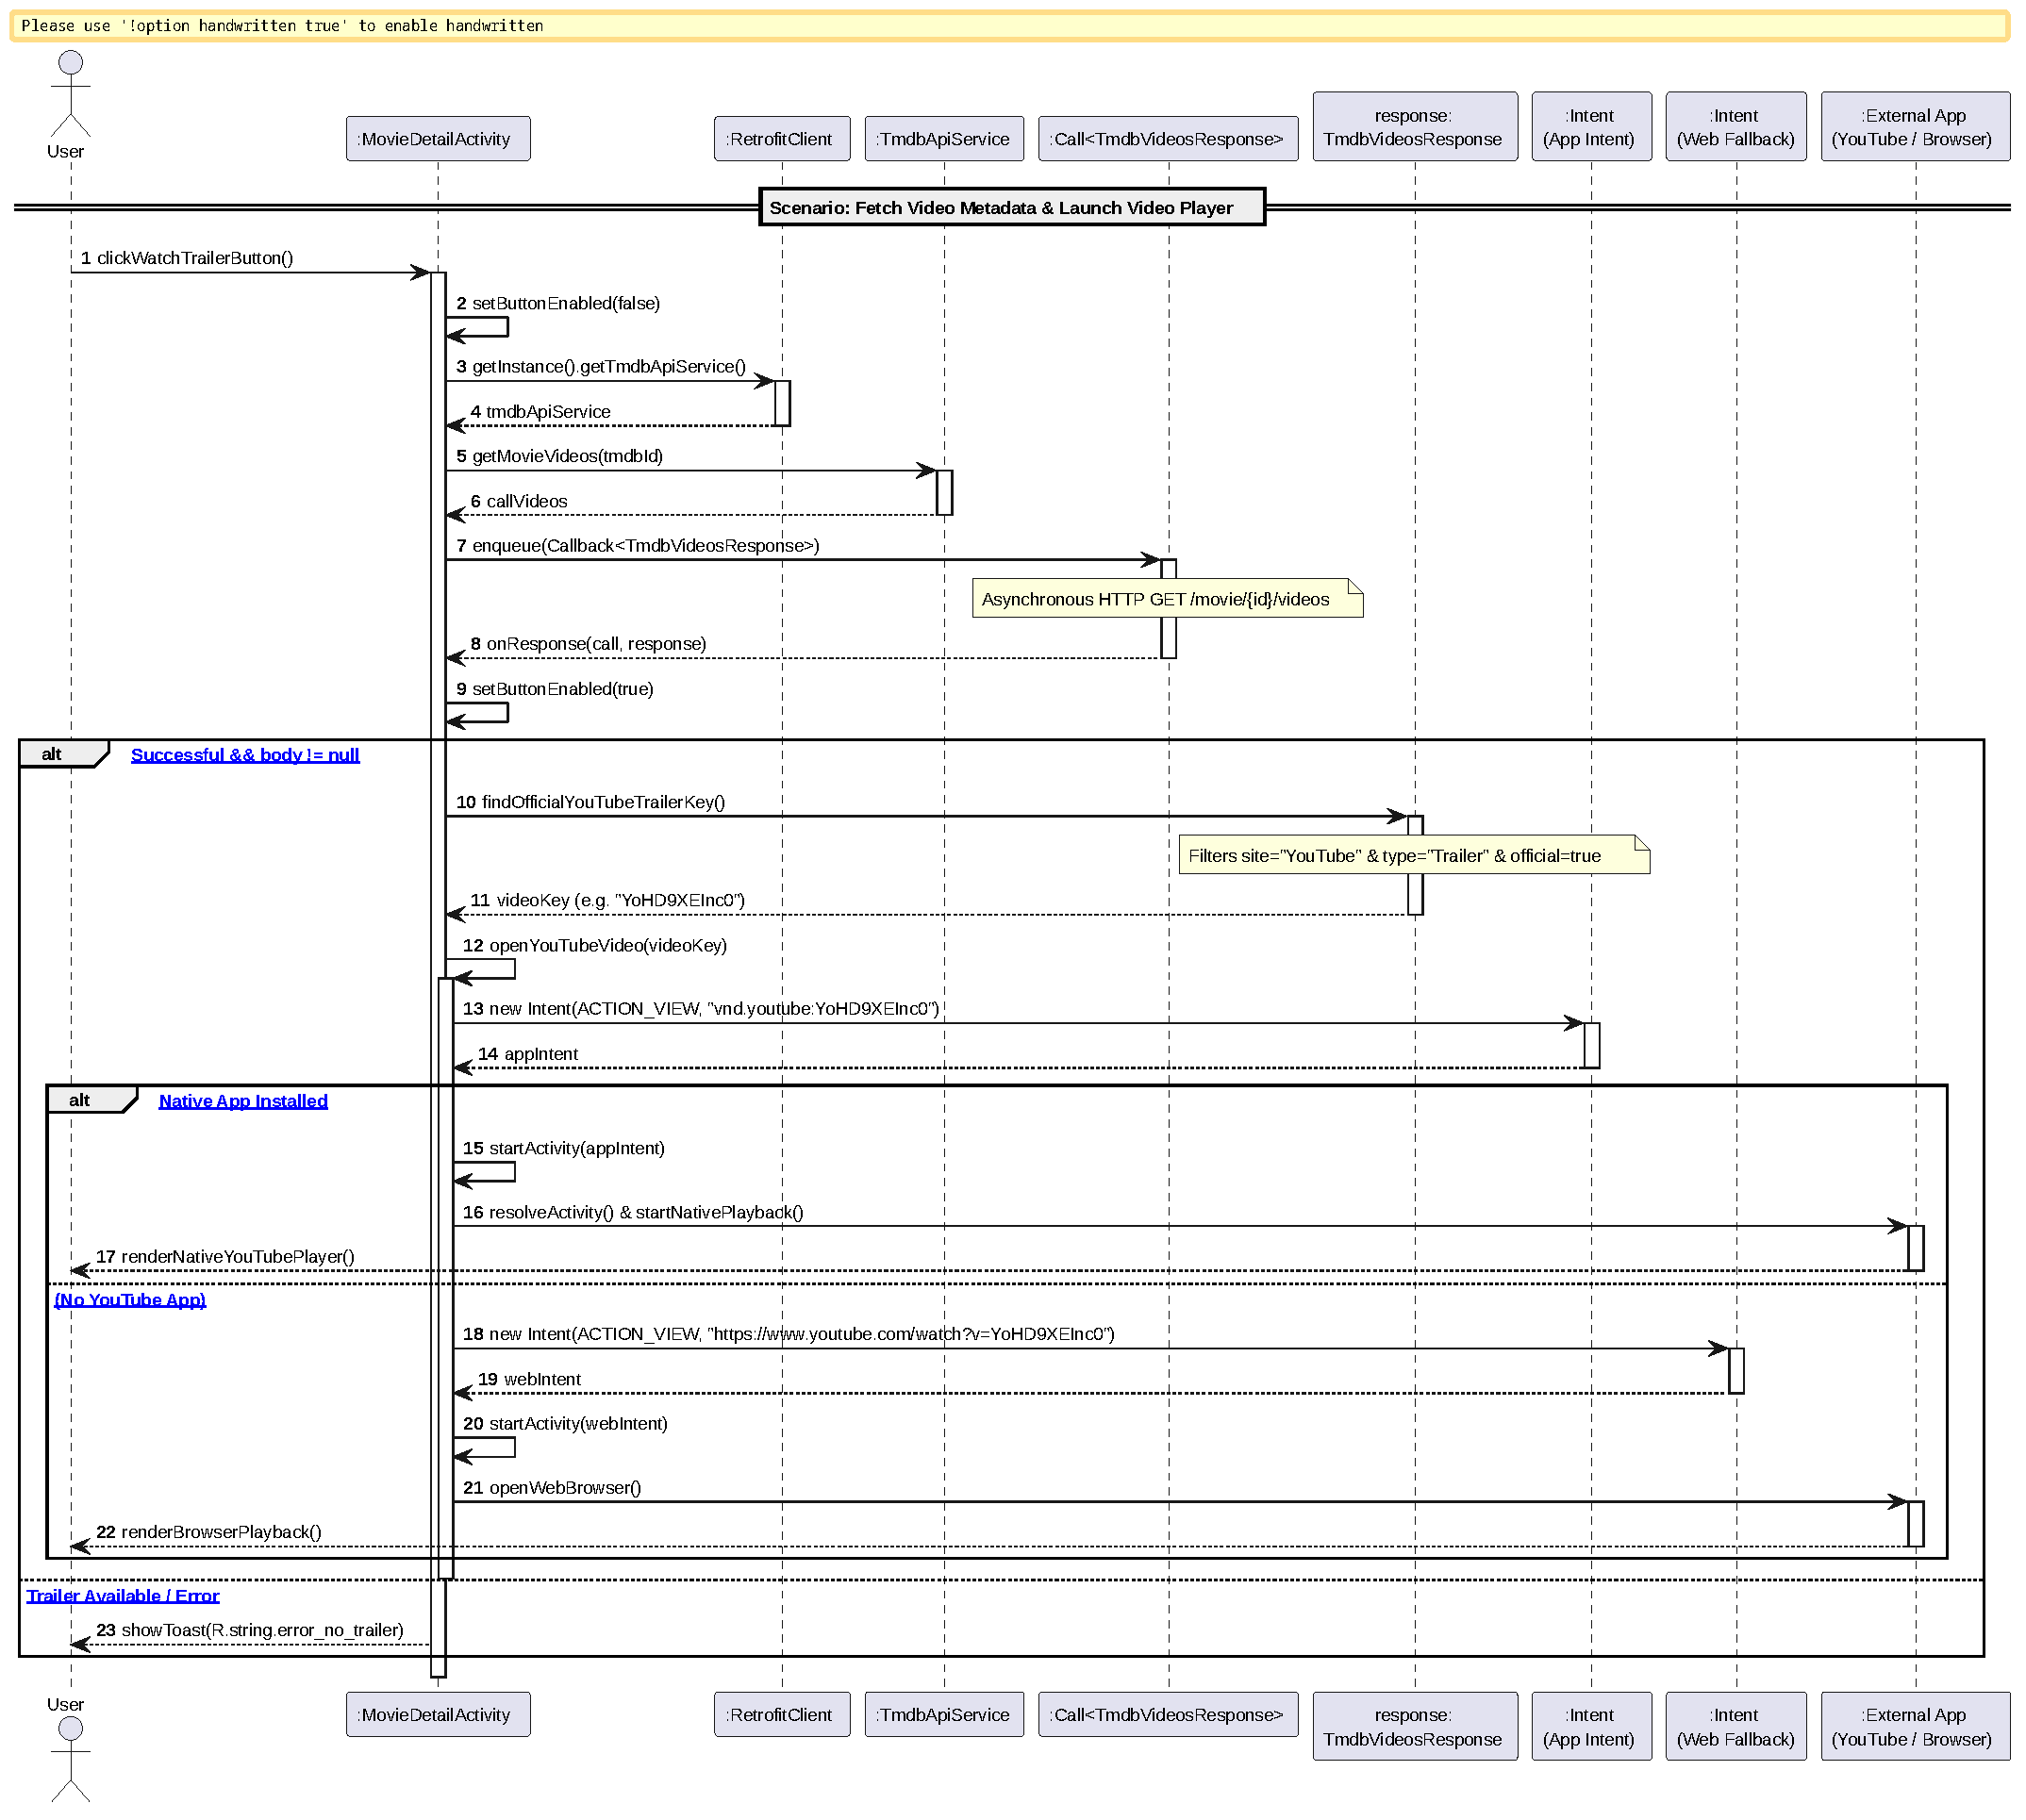
\includegraphics[width=0.85\textwidth]{figures/Use_Cases/UC10-SD.pdf}
    \caption{UC10: Official Video Trailers Design Sequence Diagram}
    \label{fig:uc10-sd}
\end{figure}

\newpage

% --------------------------------------------------------------------
% UC11
% --------------------------------------------------------------------
\vspace{0.2cm}
\noindent{\Large \textbf{Use Case 11: External Movie Card Sharing}}
\vspace{0.2cm}

The specification for UC11 is detailed in Table \ref{tab:uc11}, and its execution flow is represented in Figure \ref{fig:uc11-sd}.

\begin{center}
    \small
    \captionof{table}{Use Case 11: External Movie Sharing} \label{tab:uc11}
    \vspace{4pt}
    \begin{tabular}{@{}>{\raggedright\arraybackslash}p{2.8cm}
            >{\raggedright\arraybackslash}p{8.8cm}@{}}
        \hline
        \textbf{Actor}          & User \\
        \hline
        \textbf{Use case name}  & External Movie Card Sharing \\
        \textbf{Description}    & Formats movie title, year, synopsis, and personal review into formatted text and shares to external messaging/social apps via Intent Chooser. \\
        \textbf{Precondition}   & Movie details or saved movie card selected. \\
        \textbf{Post-condition} & System share sheet displayed; selected messaging application populated with formatted text. \\
        \textbf{Main flow}      & 
        1. User taps share icon on movie card. \newline
        2. System builds formatted message string including title, year, and overview. \newline
        3. System creates \texttt{ACTION\_SEND} intent with \texttt{text/plain} MIME type. \newline
        4. Intent wrapped in \texttt{Intent.createChooser()} to present native share dialog. \newline
        5. User selects target application (e.g., WhatsApp, Messages, Email) to complete share. \\
        \textbf{Alternative path} & 
        If user cancels the system share sheet, application resumes cleanly without side effects. \\
        \hline
    \end{tabular}
\end{center}

\begin{figure}[H]
    \centering
    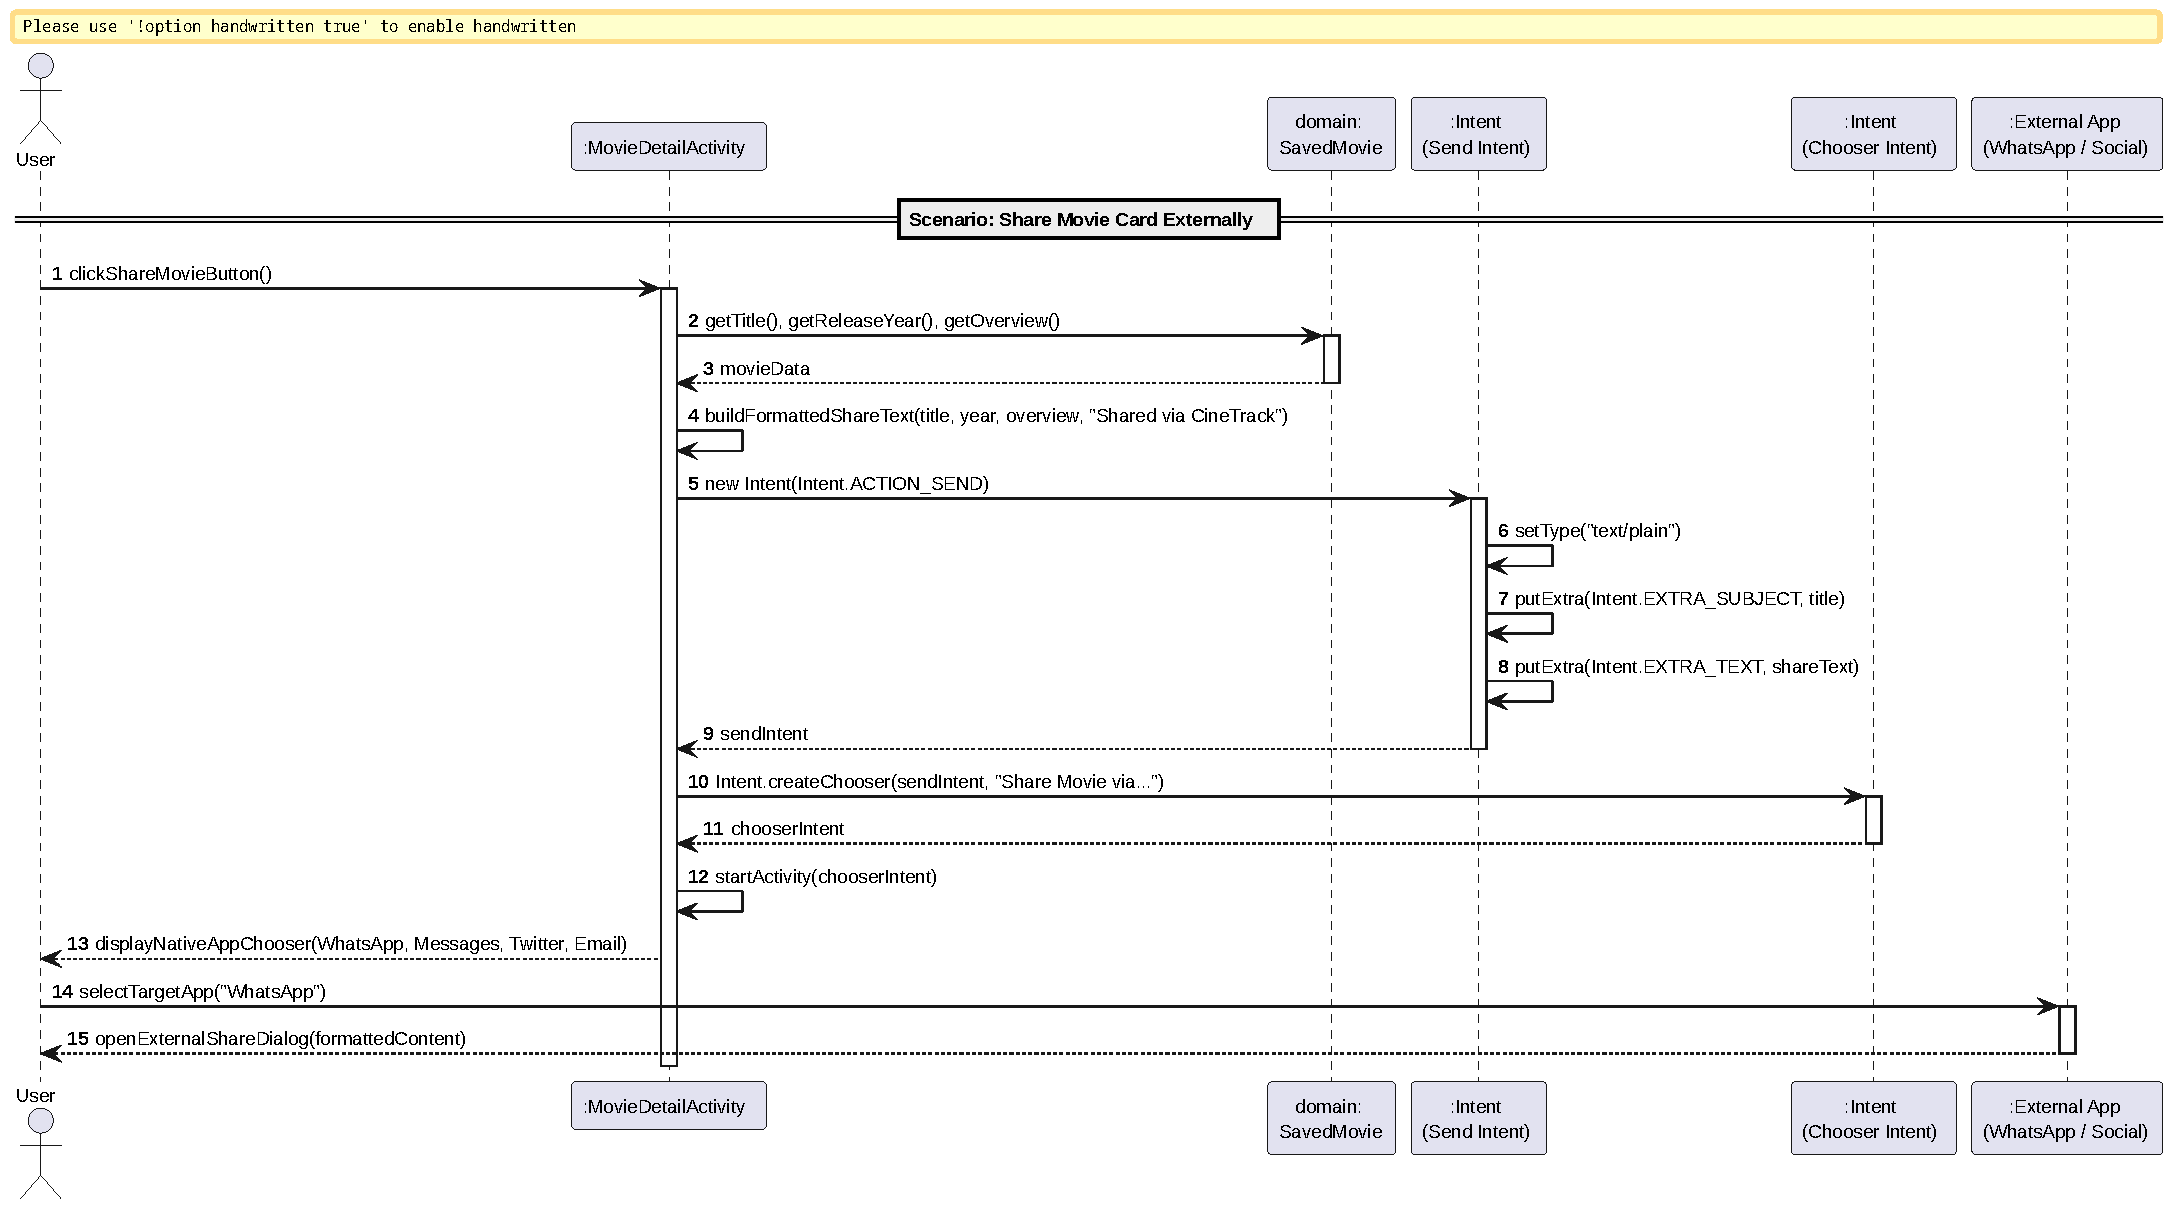
\includegraphics[width=0.85\textwidth]{figures/Use_Cases/UC11-SD.pdf}
    \caption{UC11: External Social Sharing Design Sequence Diagram}
    \label{fig:uc11-sd}
\end{figure}

\newpage

% ====================================================================
\section{Implementation and Testing}
% ====================================================================

This section presents representative excerpts from the CineTrack Java~21 codebase and from the JUnit~5 test suites. The excerpts demonstrate how the system enforces Model purity, maintains asynchronous UI Thread responsiveness, manages hardware sensors, and verifies domain integrity through automated tests.

\subsection{Pure Java 21 Domain Model and Validation}
Listing \ref{lst:cinema-model} shows the pure Java~21 \texttt{Cinema} domain entity. Notice the defensive validation checks and absence of Android SDK imports.

\begin{lstlisting}[style=javastyle,caption={Pure Java 21 Cinema Domain Entity (Cinema.java)}]
package pt.isep.dssmv.projectdroid.model;

import pt.isep.dssmv.projectdroid.exceptions.InvalidDataException;
import java.util.Objects;

public class Cinema {
    private final String fsqId;
    private final String name;
    private final double latitude;
    private final double longitude;
    private String address;
    private int distanceMeters;

    public Cinema(String fsqId, String name, double latitude, double longitude) 
            throws InvalidDataException {
        if (fsqId == null || fsqId.trim().isEmpty()) {
            throw new InvalidDataException("Cinema FSQ ID cannot be null or empty.");
        }
        if (name == null || name.trim().isEmpty()) {
            throw new InvalidDataException("Cinema name cannot be null or empty.");
        }
        this.fsqId = fsqId.trim();
        this.name = name.trim();
        this.latitude = latitude;
        this.longitude = longitude;
        this.address = "";
        this.distanceMeters = 0;
    }

    public String getFsqId() { return fsqId; }
    public String getName() { return name; }
    public double getLatitude() { return latitude; }
    public double getLongitude() { return longitude; }
    public String getAddress() { return address; }
    public void setAddress(String address) { this.address = (address != null) ? address.trim() : ""; }
    public int getDistanceMeters() { return distanceMeters; }
    public void setDistanceMeters(int distanceMeters) { this.distanceMeters = Math.max(0, distanceMeters); }

    @Override
    public boolean equals(Object o) {
        if (this == o) return true;
        if (!(o instanceof Cinema cinema)) return false;
        return Objects.equals(fsqId, cinema.fsqId);
    }

    @Override
    public int hashCode() { return Objects.hash(fsqId); }
}
\end{lstlisting}

\begin{lstlisting}[style=javastyle,caption={JUnit 5 Automated Domain Tests (CinemaTest.java)}]
package pt.isep.dssmv.projectdroid.model;

import org.junit.jupiter.api.Test;
import pt.isep.dssmv.projectdroid.exceptions.InvalidDataException;
import static org.junit.jupiter.api.Assertions.*;

public class CinemaTest {
    @Test
    public void testValidCinemaCreation() throws InvalidDataException {
        Cinema cinema = new Cinema("fsq_123", "Cinema Trindade", 41.1504, -8.6095);
        cinema.setAddress("Rua do Almada 412");
        cinema.setDistanceMeters(850);

        assertEquals("fsq_123", cinema.getFsqId());
        assertEquals("Cinema Trindade", cinema.getName());
        assertEquals(41.1504, cinema.getLatitude(), 0.0001);
        assertEquals(-8.6095, cinema.getLongitude(), 0.0001);
        assertEquals("Rua do Almada 412", cinema.getAddress());
        assertEquals(850, cinema.getDistanceMeters());
    }

    @Test
    public void testEmptyFsqIdThrowsException() {
        assertThrows(InvalidDataException.class, () -> new Cinema("", "Cinema 1", 41.15, -8.60));
        assertThrows(InvalidDataException.class, () -> new Cinema(null, "Cinema 1", 41.15, -8.60));
    }

    @Test
    public void testEmptyNameThrowsException() {
        assertThrows(InvalidDataException.class, () -> new Cinema("fsq_123", "   ", 41.15, -8.60));
    }
}
\end{lstlisting}

\newpage

\subsection{Geospatial Mapping: Foursquare REST API and OSMDroid Map}
Listing \ref{lst:cinemas-activity} shows the integration of modern Foursquare Places API (Bearer authentication and version header \texttt{2025-06-17}) and OSMDroid polygon rendering for search radius visualization.

\begin{lstlisting}[style=javastyle,caption={OSMDroid Radius and Cinema Markers (CinemasActivity.java)}]
private void centerMapAndDrawRadius(GeoPoint userPoint, int radiusKm) {
    mapView.getController().setZoom(computeZoomLevel(radiusKm));
    mapView.getController().setCenter(userPoint);

    mapView.getOverlays().clear();
    cinemaMarkers.clear();

    // 1. Translucent Blue Radius Circumference Polygon
    double radiusMeters = radiusKm * 1000.0;
    Polygon circle = new Polygon(mapView);
    circle.setPoints(Polygon.pointsAsCircle(userPoint, radiusMeters));
    circle.setFillColor(0x262196F3);   // 15% alpha translucent blue
    circle.setStrokeColor(0xFF2196F3); // Solid blue border
    circle.setStrokeWidth(3.0f);
    mapView.getOverlays().add(circle);

    // 2. User Location Marker
    Marker userMarker = new Marker(mapView);
    userMarker.setPosition(userPoint);
    userMarker.setTitle(getString(R.string.label_user_location));
    userMarker.setIcon(ContextCompat.getDrawable(this, R.drawable.ic_my_location));
    mapView.getOverlays().add(userMarker);

    mapView.invalidate();
}

private void queryFoursquareCinemas(double lat, double lon, int radiusKm) {
    String latLng = lat + "," + lon;
    int radiusMeters = Math.min(radiusKm * 1000, 100000);

    RetrofitClient.getInstance().getFoursquareApiService()
        .searchNearbyCinemas(latLng, "cinema", "10024", radiusMeters, "DISTANCE", 20)
        .enqueue(new Callback<FsqPlacesResponse>() {
            @Override
            public void onResponse(Call<FsqPlacesResponse> call, Response<FsqPlacesResponse> resp) {
                progressBar.setVisibility(View.GONE);
                if (resp.isSuccessful() && resp.body() != null) {
                    List<Cinema> domainCinemas = mapToDomainCinemas(resp.body().getResults());
                    adapter.setCinemas(domainCinemas);
                    plotCinemaMarkersOnMap(domainCinemas);
                }
            }
            @Override
            public void onFailure(Call<FsqPlacesResponse> call, Throwable t) {
                progressBar.setVisibility(View.GONE);
            }
        });
}
\end{lstlisting}

\newpage

\subsection{Hardware Sensor Lifecycle: Accelerometer Shake Detection}
Listing \ref{lst:shake-lifecycle} demonstrates battery preservation rules by registering the sensor listener in \texttt{onResume()} and immediately unregistering in \texttt{onPause()}.

\begin{lstlisting}[style=javastyle,caption={Accelerometer Lifecycle Discipline (MainActivity.java)}]
@Override
protected void onResume() {
    super.onResume();
    // AC04: Strictly register accelerometer in onResume()
    if (sensorManager != null && accelerometer != null && shakeDetector != null) {
        sensorManager.registerListener(shakeDetector, accelerometer, SensorManager.SENSOR_DELAY_UI);
    }
}

@Override
protected void onPause() {
    super.onPause();
    // AC04: Strictly unregister accelerometer in onPause() to preserve battery
    if (sensorManager != null && shakeDetector != null) {
        sensorManager.unregisterListener(shakeDetector);
    }
    if (currentShakeDialog != null && currentShakeDialog.isShowing()) {
        currentShakeDialog.dismiss();
    }
    isShakeDialogOpen = false;
}
\end{lstlisting}

\begin{lstlisting}[style=javastyle,caption={Multi-Peak Shake Detection Algorithm (ShakeDetector.java)}]
@Override
public void onSensorChanged(SensorEvent event) {
    if (event.sensor.getType() != Sensor.TYPE_ACCELEROMETER) return;

    float x = event.values[0] / SensorManager.GRAVITY_EARTH;
    float y = event.values[1] / SensorManager.GRAVITY_EARTH;
    float z = event.values[2] / SensorManager.GRAVITY_EARTH;

    float gForce = (float) Math.sqrt(x * x + y * y + z * z);
    long now = System.currentTimeMillis();

    if (gForce > shakeThresholdG) {
        if (now - lastShakeTriggerTimestamp < SHAKE_COOLDOWN_MS) return;
        if (lastShakePeakTimestamp > 0 && (now - lastShakePeakTimestamp) < SHAKE_SLOP_TIME_MS) return;

        shakeCount++;
        lastShakePeakTimestamp = now;

        if (shakeCount >= 2) {
            shakeCount = 0;
            lastShakeTriggerTimestamp = now;
            if (listener != null) listener.onShake();
        }
    }
}
\end{lstlisting}

\newpage

\subsection{Pure Java 21 Collection Sorting and Filtering}
Listing \ref{lst:filter-sorter} shows the functional comparator implementation used in US9.

\begin{lstlisting}[style=javastyle,caption={Functional Comparator Implementation (SavedMovieFilterSorter.java)}]
public final class SavedMovieFilterSorter {
    public static final Comparator<SavedMovie> COMPARATOR_TITLE_ASC =
        Comparator.comparing((SavedMovie m) -> m.getTitle() == null ? "" : m.getTitle(), String.CASE_INSENSITIVE_ORDER);

    public static final Comparator<SavedMovie> COMPARATOR_RATING_DESC =
        Comparator.comparingDouble((SavedMovie m) -> (m.getRating() != null) ? m.getRating().getScore() : -1.0)
            .reversed()
            .thenComparing(COMPARATOR_TITLE_ASC);

    public static List<SavedMovie> filterAndSort(List<SavedMovie> movies, WatchStatus status,
                                                 String query, SavedMovieSortOption sortOption) {
        if (movies == null) return new ArrayList<>();
        return movies.stream()
            .filter(m -> status == null || m.getStatus() == status)
            .filter(m -> query == null || query.trim().isEmpty() ||
                         m.getTitle().toLowerCase().contains(query.trim().toLowerCase()))
            .sorted(getComparator(sortOption))
            .collect(Collectors.toList());
    }
}
\end{lstlisting}

% ====================================================================
\section{Conclusion}
% ====================================================================
This technical report presented the comprehensive specification, architectural design, implementation, and verification of the \textbf{CineTrack} mobile application. Over the course of the project, all 11 User Stories assigned across the team were completed with 100\% functionality and verified against automated test suites and live hardware deployments.

The application successfully reconciles disparate mobile concerns into an integrated architecture:
\begin{itemize}
    \item \textbf{Architectural Decoupling:} Strict adherence to MVC preserved the purity of domain business logic in Java~21 without framework contamination, making 53 automated unit tests run instantaneously.
    \item \textbf{UI Thread Responsiveness:} Mandatory asynchronous execution via Retrofit~2 \texttt{.enqueue()} and SharedPreferences \texttt{.apply()} eradicated ANR risks across network and storage boundaries.
    \item \textbf{Hardware and Battery Protection:} The accelerometer-based \textit{Shake to Suggest} and native GPS tracking adhere to Android lifecycle discipline, preventing sensor battery drain when activities are paused.
    \item \textbf{Free Geospatial Mapping:} Integrating OSMDroid alongside modern Foursquare Places API enabled full interactive cinema mapping with custom radius circles without requiring paid Google Cloud keys.
\end{itemize}

Future enhancements could expand CineTrack by introducing social friend lists, push notifications for theatrical releases, and offline caching of movie details via Android Room database. In its current release, CineTrack stands as a complete, robust, and academically sound mobile solution demonstrating software engineering excellence in Android native development.

\newpage

% ====================================================================
% BIBLIOGRAFIA
% ====================================================================
\renewcommand{\refname}{References}

\begin{thebibliography}{9}

\bibitem{sousa_dssmv_2026}
P.~B. Sousa, ``Lecture Slides and Pedagogical Guidelines for DSSMV (Desenvolvimento de Software e Sistemas M\'oveis),'' Instituto Superior de Engenharia do Porto (ISEP), Polytechnic of Porto, 2026.

\bibitem{horstmann_bigjava}
C.~S. Horstmann, \emph{Big Java: Early Objects}, 6th~ed.\hskip 1em plus 0.5em minus 0.4em\relax Wiley, 2015.

\bibitem{android_lifecycle}
Android Developers, ``Processes and Application Lifecycle Documentation,'' Google LLC, \url{https://developer.android.com/guide/components/activities/activity-lifecycle}.

\bibitem{tmdb_api}
The Movie Database (TMDB), ``TMDB REST API Documentation v3,'' \url{https://developer.themoviedb.org/docs}.

\bibitem{fsq_places_api}
Foursquare Labs, Inc., ``Foursquare Places API Documentation (v2025-06-17),'' \url{https://location.foursquare.com/developer/reference/places-api-overview}.

\bibitem{osmdroid_docs}
OSMDroid Community, ``OpenStreetMap-Tools for Android Documentation (v6.1.20),'' \url{https://github.com/osmdroid/osmdroid}.

\end{thebibliography}

\end{document}
